\documentclass{article}
\usepackage{graphicx} 
\usepackage{multirow}
\usepackage{listings}
\lstset{
  breaklines=true,
  %language=Python
}
\usepackage{float}
\usepackage{caption}
\usepackage{subcaption}
\usepackage{amssymb}
\usepackage{amsmath}
\usepackage{cases}
\usepackage{verbatim}
\usepackage{hyperref}

\title{Optimization Labs}
\author{Manuela Corte Pause}

\begin{document}

\maketitle

\tableofcontents
\newpage

\section{Grid Search, Random Seach, Nealder-Mead and Powell}
\subsection{Grid Search}
\label{sec:grid-search}

Grid search performs an uninformed search on the entire search space of the optimization function. If we decrease the step size (or equivalently increase the number of steps), we would be able to eventually find the global minimum. However, this comes at the cost of increased computational time which is especially problematic for complex functions. Moreover, in high-dimensional spaces, the number of steps required to find the global minimum increases exponentially.

For example below \ref{fig:gs-100} we report the results of grid search for the Rastrigin function in 2D which is a non-convex highly multimodal function and compare then with the much more simple Hypersphere function. We can see that with 100 steps we are able to get an approximation that is rougly comparable despite the difference in complexity of the two functions.
\begin{figure}[H]
    \begin{subfigure}{0.5\textwidth}
        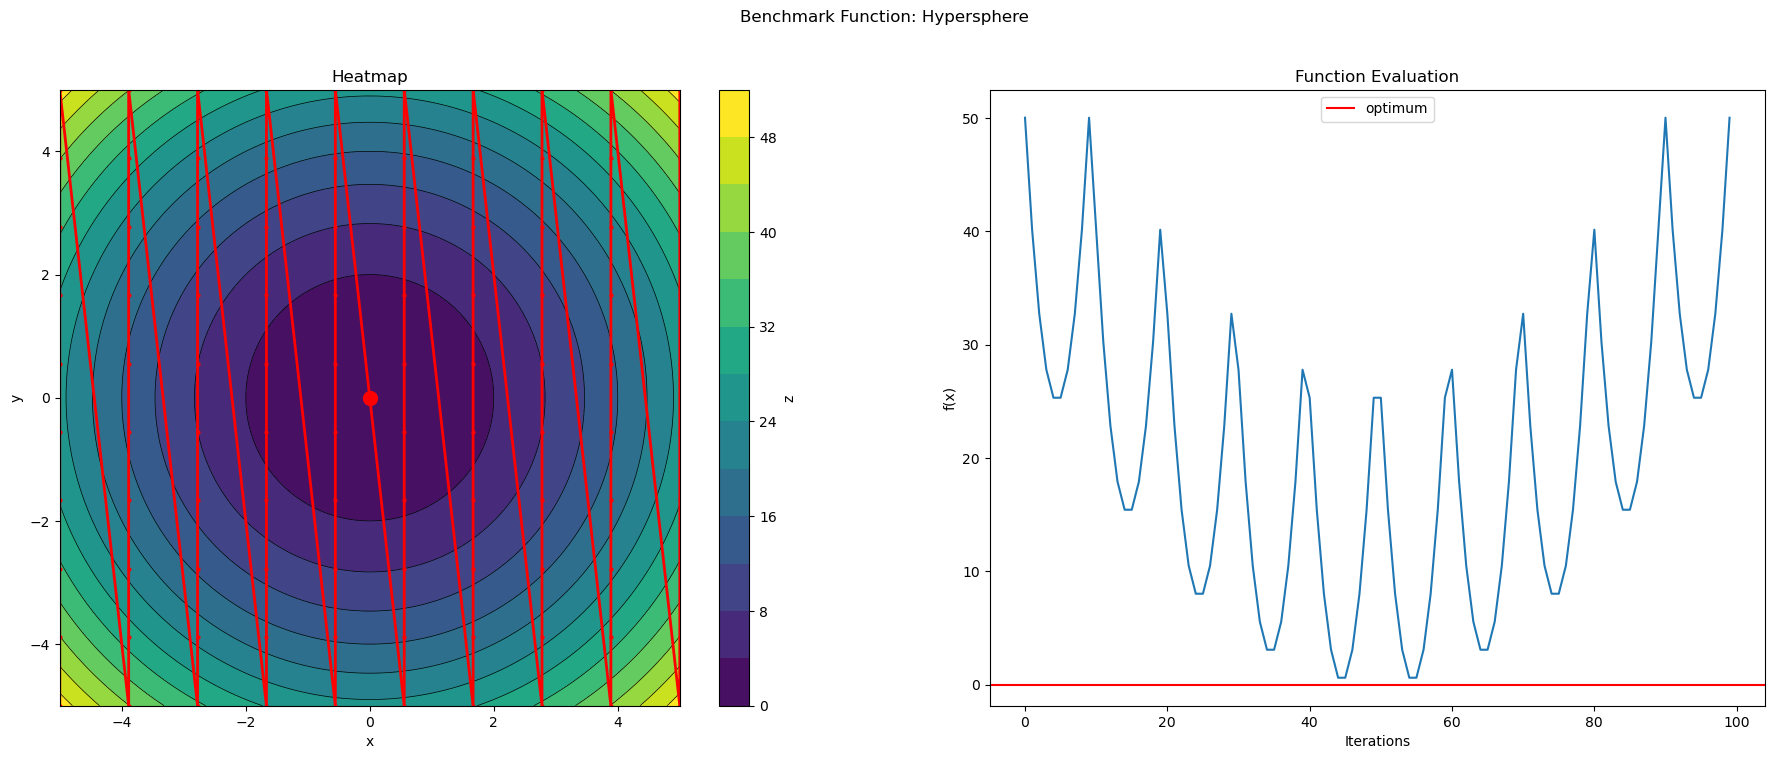
\includegraphics[width=\textwidth]{lab1/imgs/gs_sphere_100.png}
        \caption{Hypersphere function with 100 steps}
    \end{subfigure}
    \begin{subfigure}{0.5\textwidth}
        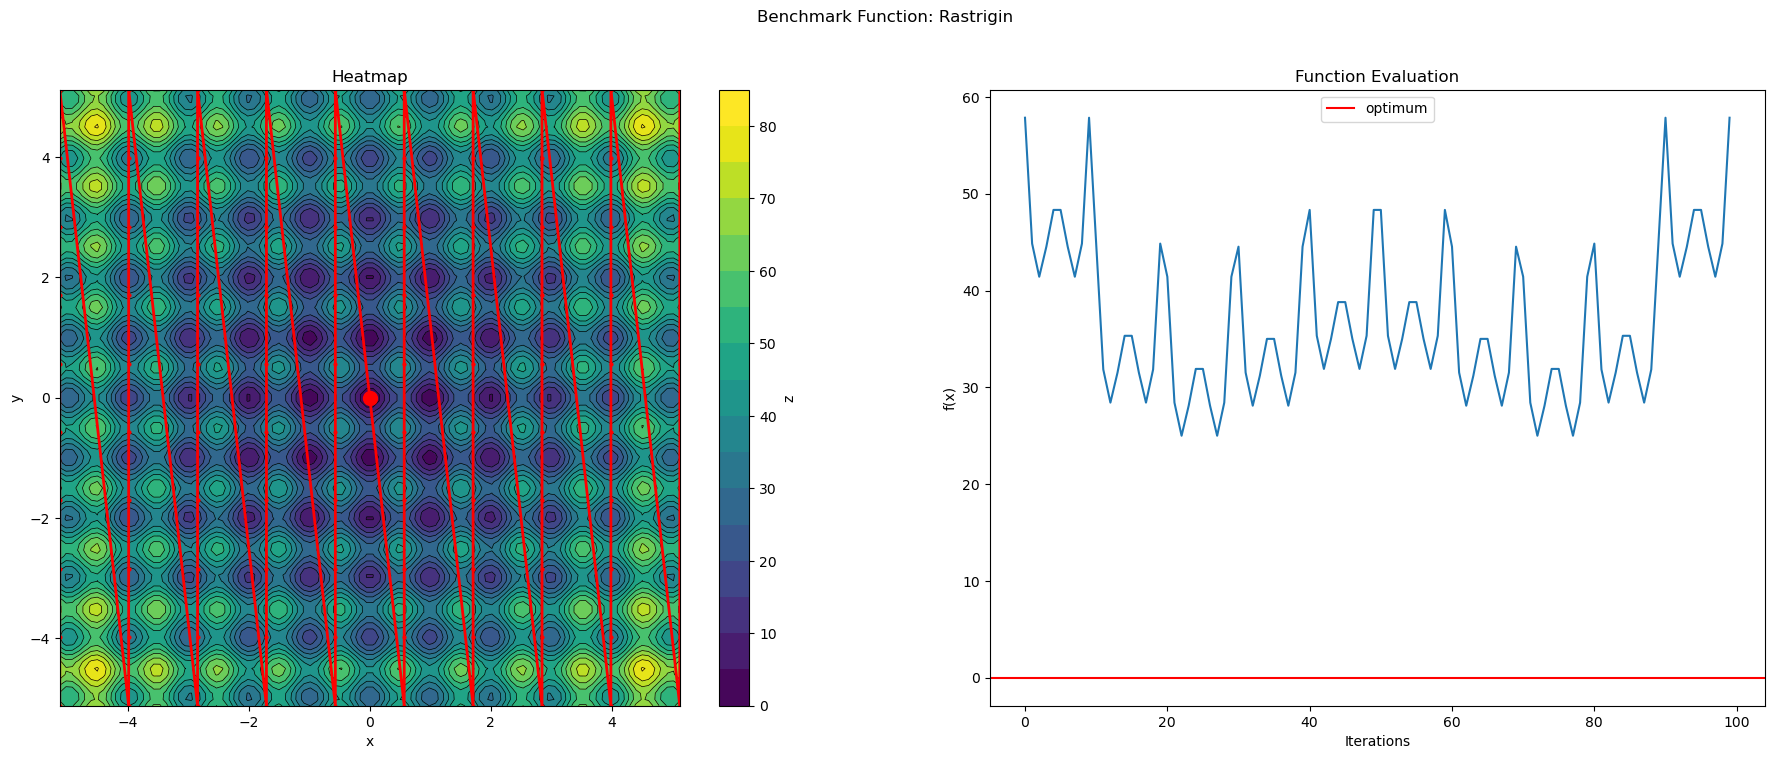
\includegraphics[width=\textwidth]{lab1/imgs/gs_rastrigin_100.png}
        \caption{Rastrigin function with 100 steps}
    \end{subfigure}
    \caption{Comparison between grid search on the Hypersphere and Rastrigin functions}
    \label{fig:gs-100}
\end{figure}

Given that an uniformed search is performed, this means that there is no risk of getting stuck in a local minima but at the same time no information abount the actual shape of the function is used to guide the search. This means that the search is not efficient and the number of steps required to find the global minimum can be very high. At the same it time it can also happen that a higher number of steps doesn't result in an improved solution simply because the discretization of the search space ends up sampling points with a worse objective function. For example we can see this in the example below \ref{fig:gs-ackley} with the Ackley function where 10 steps are able to perfectly find the minimum while 100 steps can't (this is mainly due to the fact the search space is a square and the minimum is exactly in zero so the discretization with 10 steps contains exactly the minimum).

\begin{figure}[H]
    \begin{subfigure}{0.5\textwidth}
        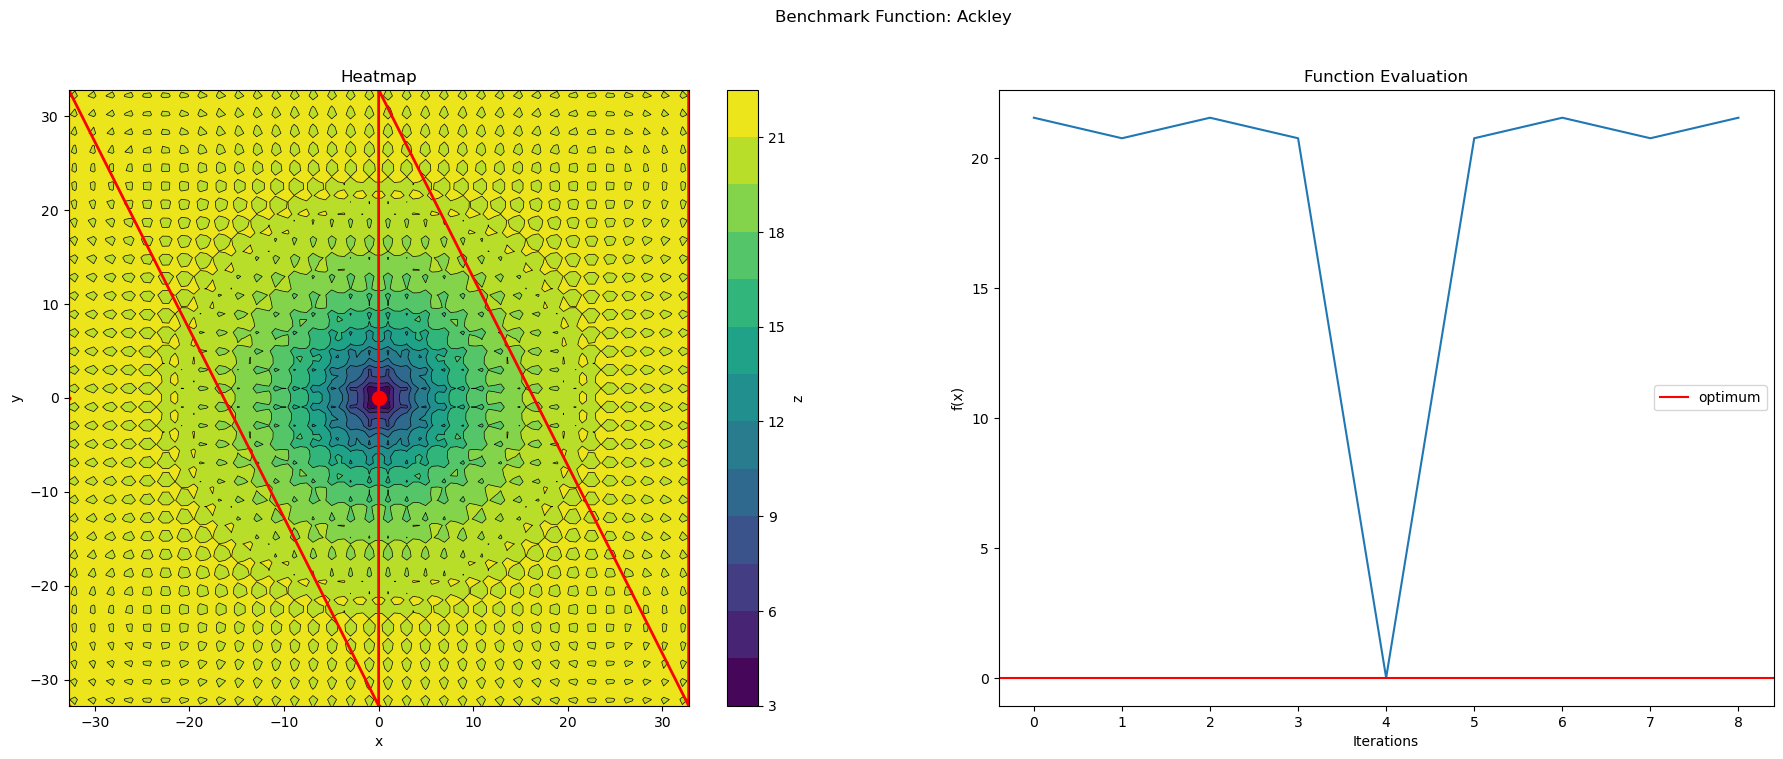
\includegraphics[width=\textwidth]{lab1/imgs/gs_ackley_10.png}
        \caption{Ackley function with 10 steps}
    \end{subfigure}
    \begin{subfigure}{0.5\textwidth}
        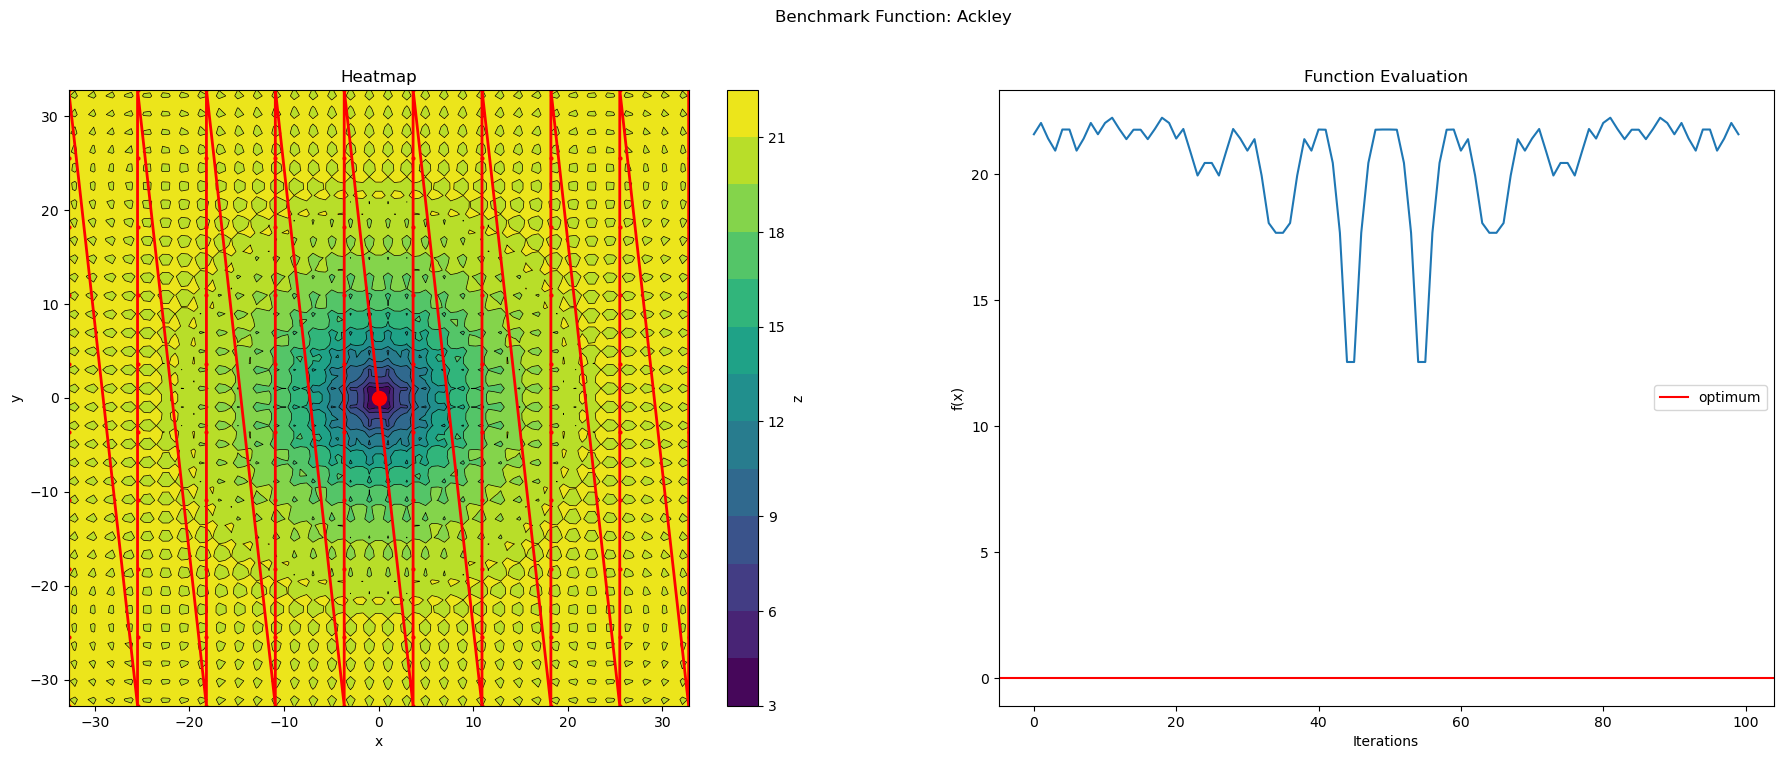
\includegraphics[width=\textwidth]{lab1/imgs/gs_ackley_100.png}
        \caption{Ackley function with 100 steps}
    \end{subfigure}
    \caption{Grid search on the Ackley function}
    \label{fig:gs-ackley}
\end{figure}


\subsection{Random Search}
\label{sec:random-search}
Random search is an uninformed search method that samples the search space randomly.
Given that the samples are taken randomly in the search space, all functions are equally hard to optimize (assuming that all fitness functions are equally computationally hard). For example below \ref{fig:rs-100} we can see different functions, all with 100 samples and see that the results are comparable in terms of the quality of the solution found regarless of function.

\begin{figure}[H]
    \begin{subfigure}{0.5\textwidth}
        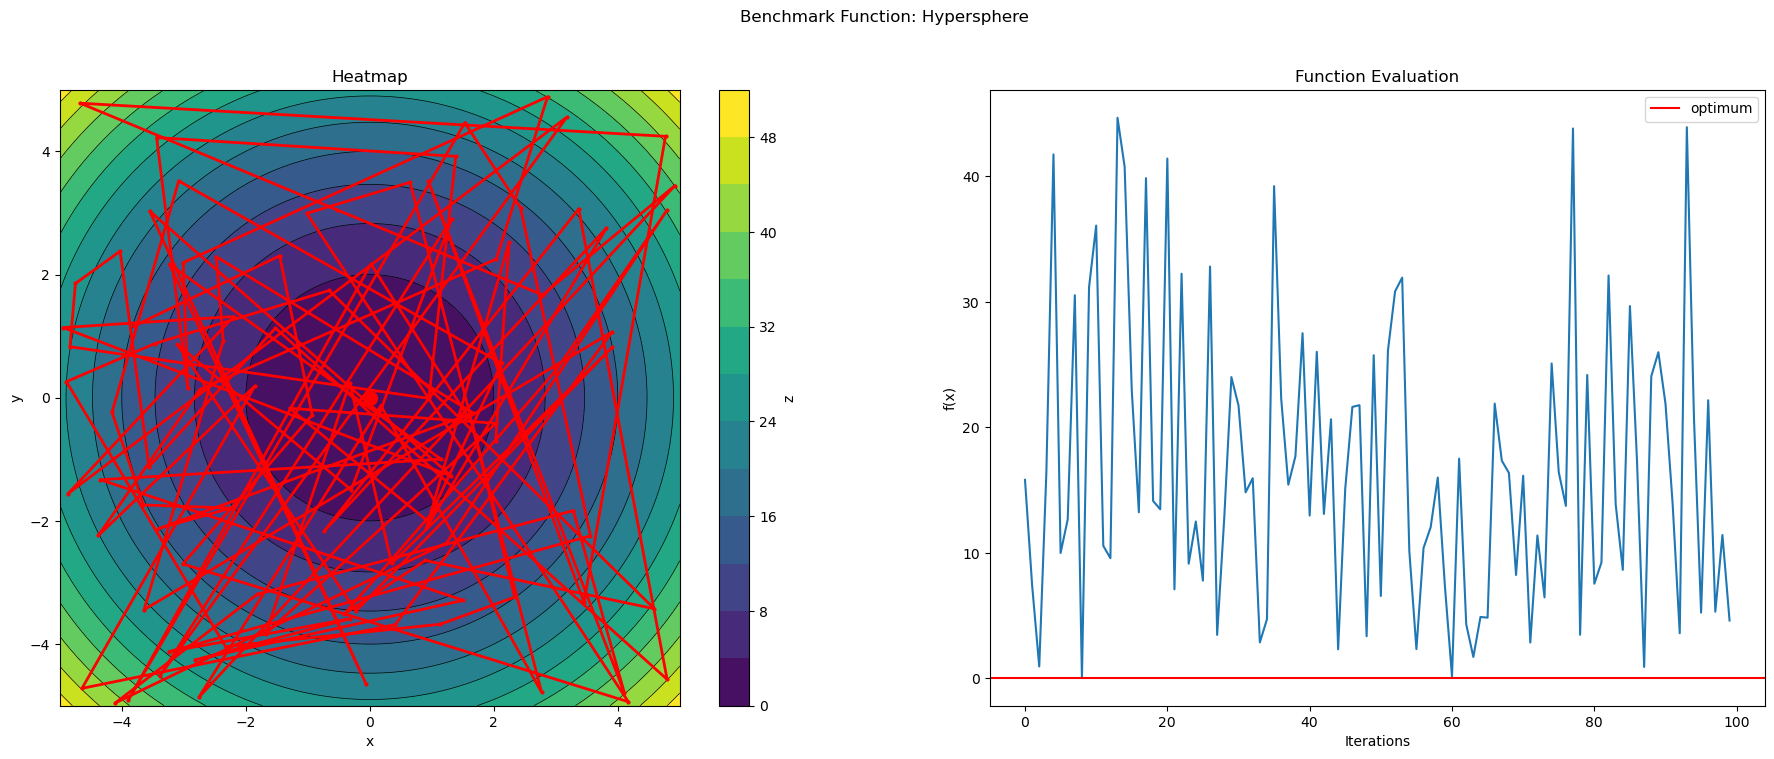
\includegraphics[width=\textwidth]{lab1/imgs/rs_sphere_100.png}
        \caption{Hypersphere}
    \end{subfigure}
    \begin{subfigure}{0.5\textwidth}
        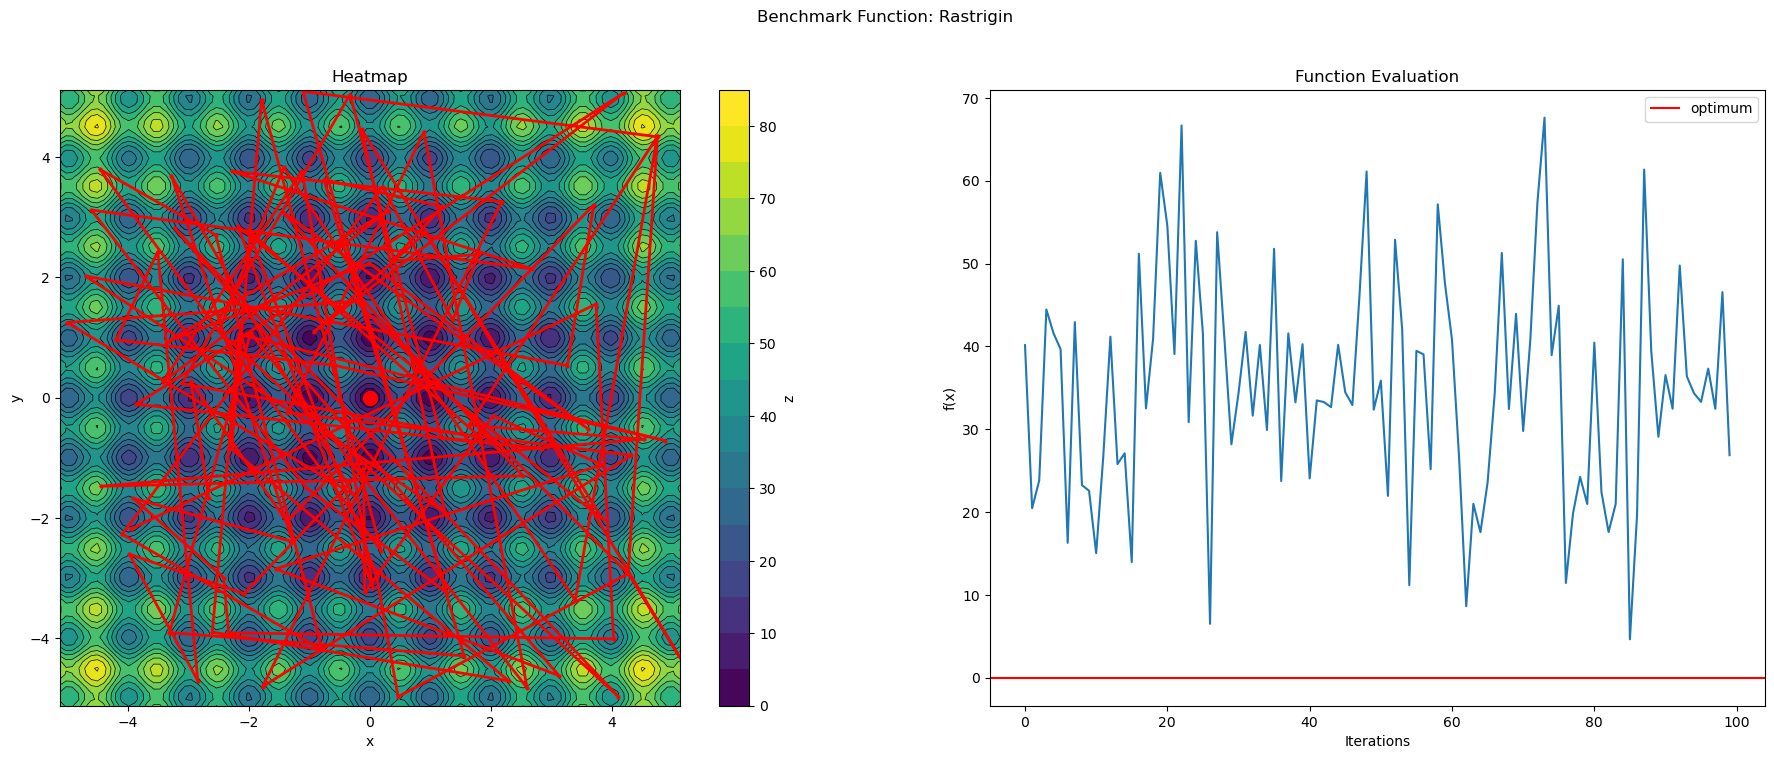
\includegraphics[width=\textwidth]{lab1/imgs/rs_rastrigin_100.png}
        \caption{Rastrigin}
    \end{subfigure} \\
    \begin{subfigure}{\textwidth}
        \centering
        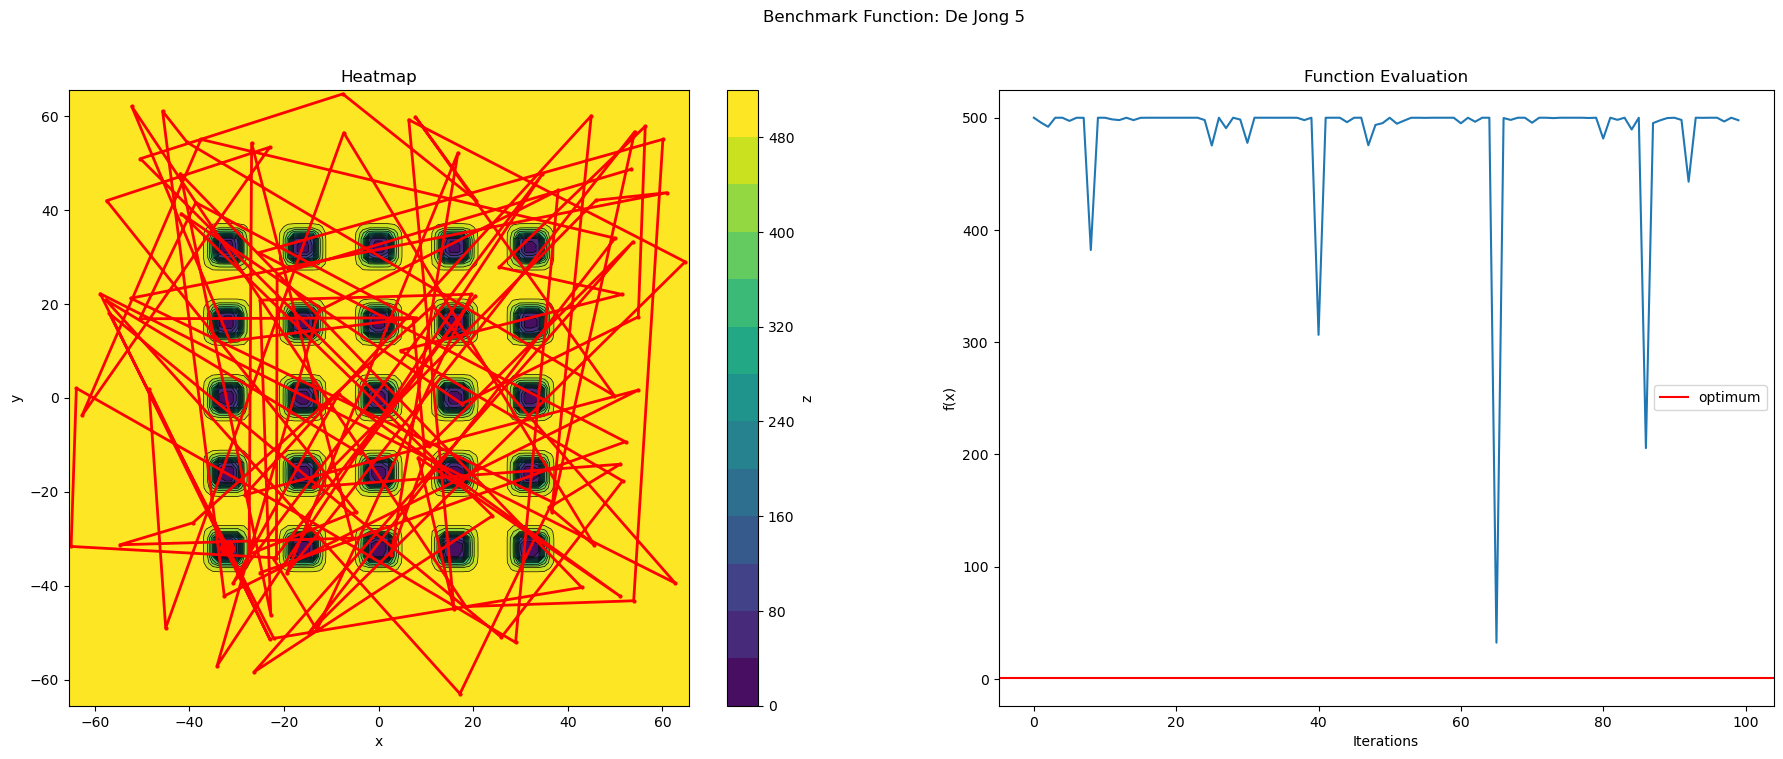
\includegraphics[width=0.5\textwidth]{lab1/imgs/rs_dejong_100.png}
        \caption{DeJong5}
    \end{subfigure}
    \caption{Random search on different functions with 100 samples}
    \label{fig:rs-100}
\end{figure}

\subsection{Powell}
\label{sec:powell}
Powell's method is a conjugate direction method that uses a set of directions to perform a line search. The directions are updated at each iteration to minimize the function. The method is only guaranteed to find a local minimum but in practice it is often able to find the global minimum as well. For example, in the image below \ref{fig:pw} we can see the results of Powell's method on the Rastrigin function, where the method is able to find the global minimum, and the DeJong5 function, where it's not able to, even if the functions are both multimodal.

\begin{figure}[H]
    \begin{subfigure}{0.5\textwidth}
        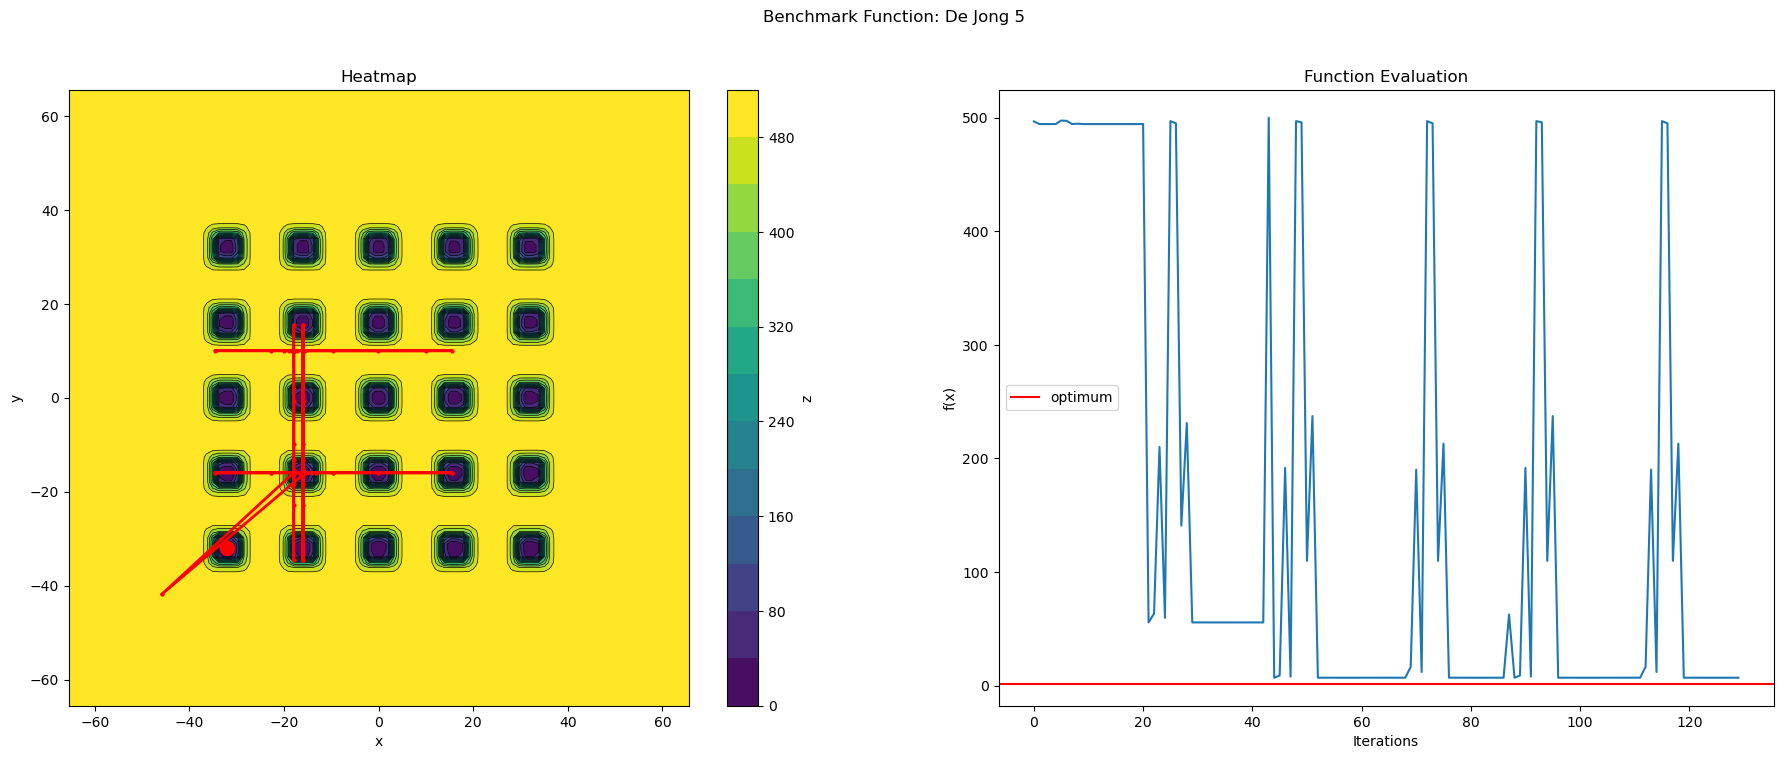
\includegraphics[width=\textwidth]{lab1/imgs/pw_dejong.png}
        \caption{DeJong5}
    \end{subfigure}
    \begin{subfigure}{0.5\textwidth}
        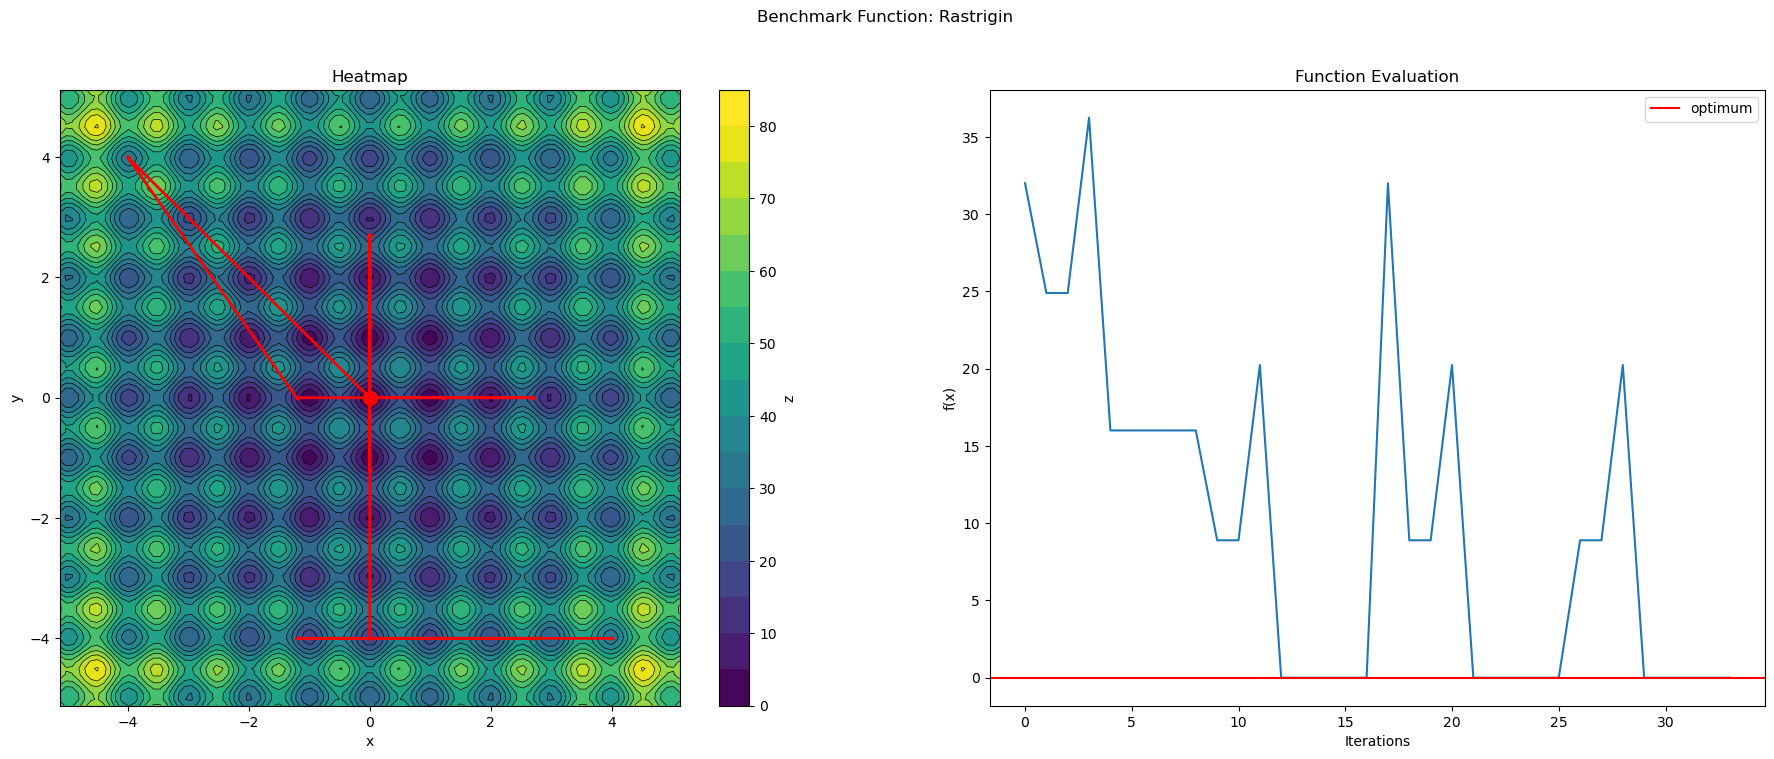
\includegraphics[width=\textwidth]{lab1/imgs/pw_rastrigin.png}
        \caption{Rastrigin}
    \end{subfigure}
    \caption{Powell's method comparison}
    \label{fig:pw}
\end{figure}

Another important aspect of Powell's method is the choice of the initial directions. In the graph below \ref{fig:ackley} we can see that even if the method is able to find the global minimum in both scenarios, the choice of the initial directions has an impact on the number of iterations required to find the minimum.

\begin{figure}[H]
    \begin{subfigure}{0.5\textwidth}
        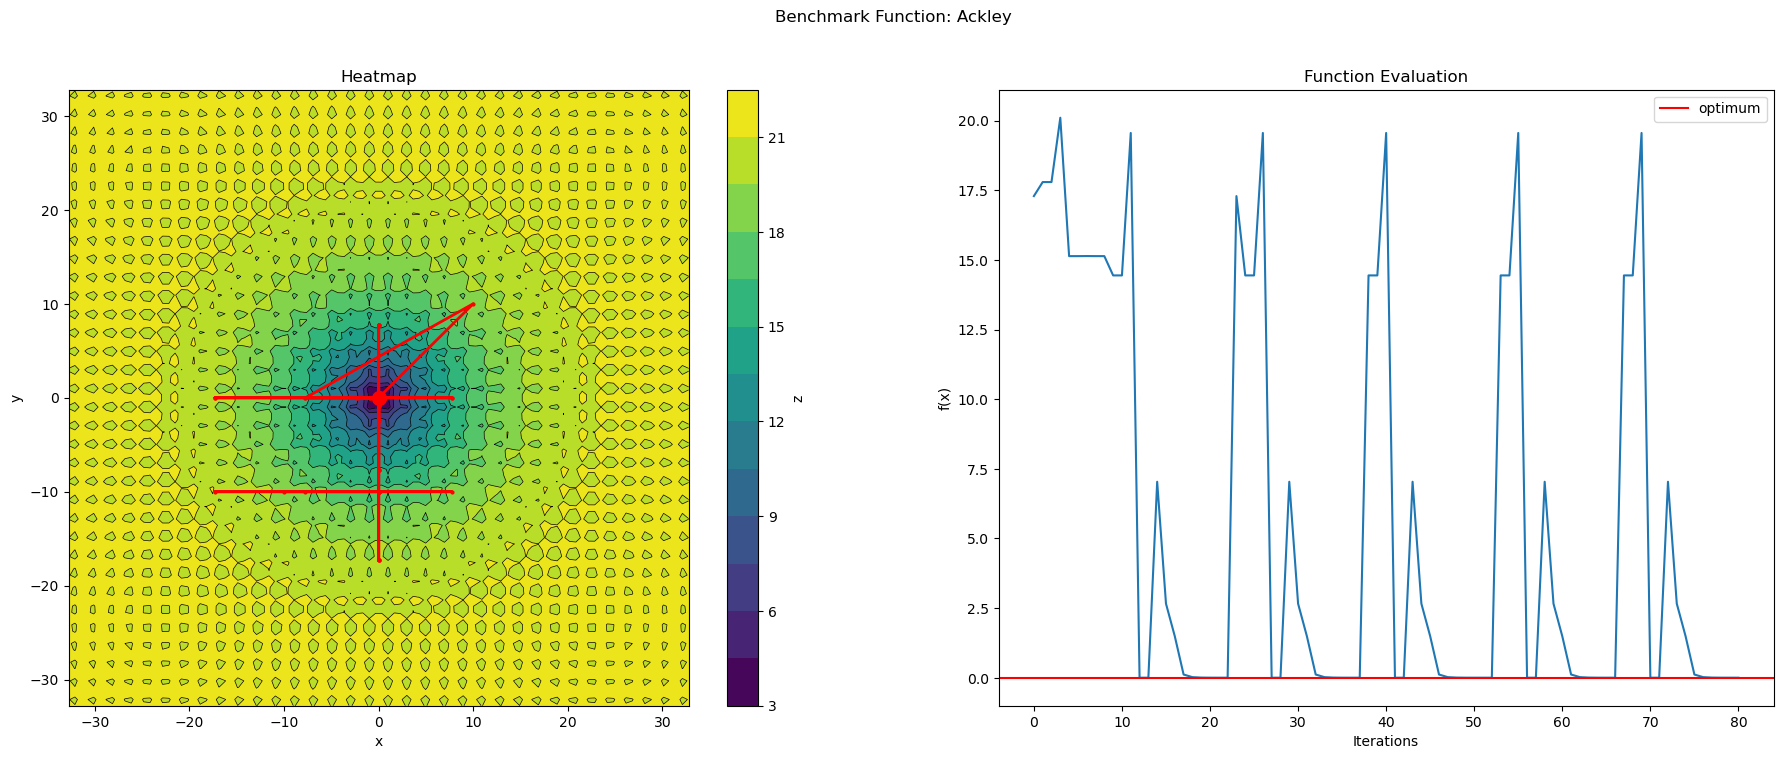
\includegraphics[width=\textwidth]{lab1/imgs/pw_ackley.png}
        \caption{Ackley with directions [[1, 0],[0,1]]}
    \end{subfigure}
    \begin{subfigure}{0.5\textwidth}
        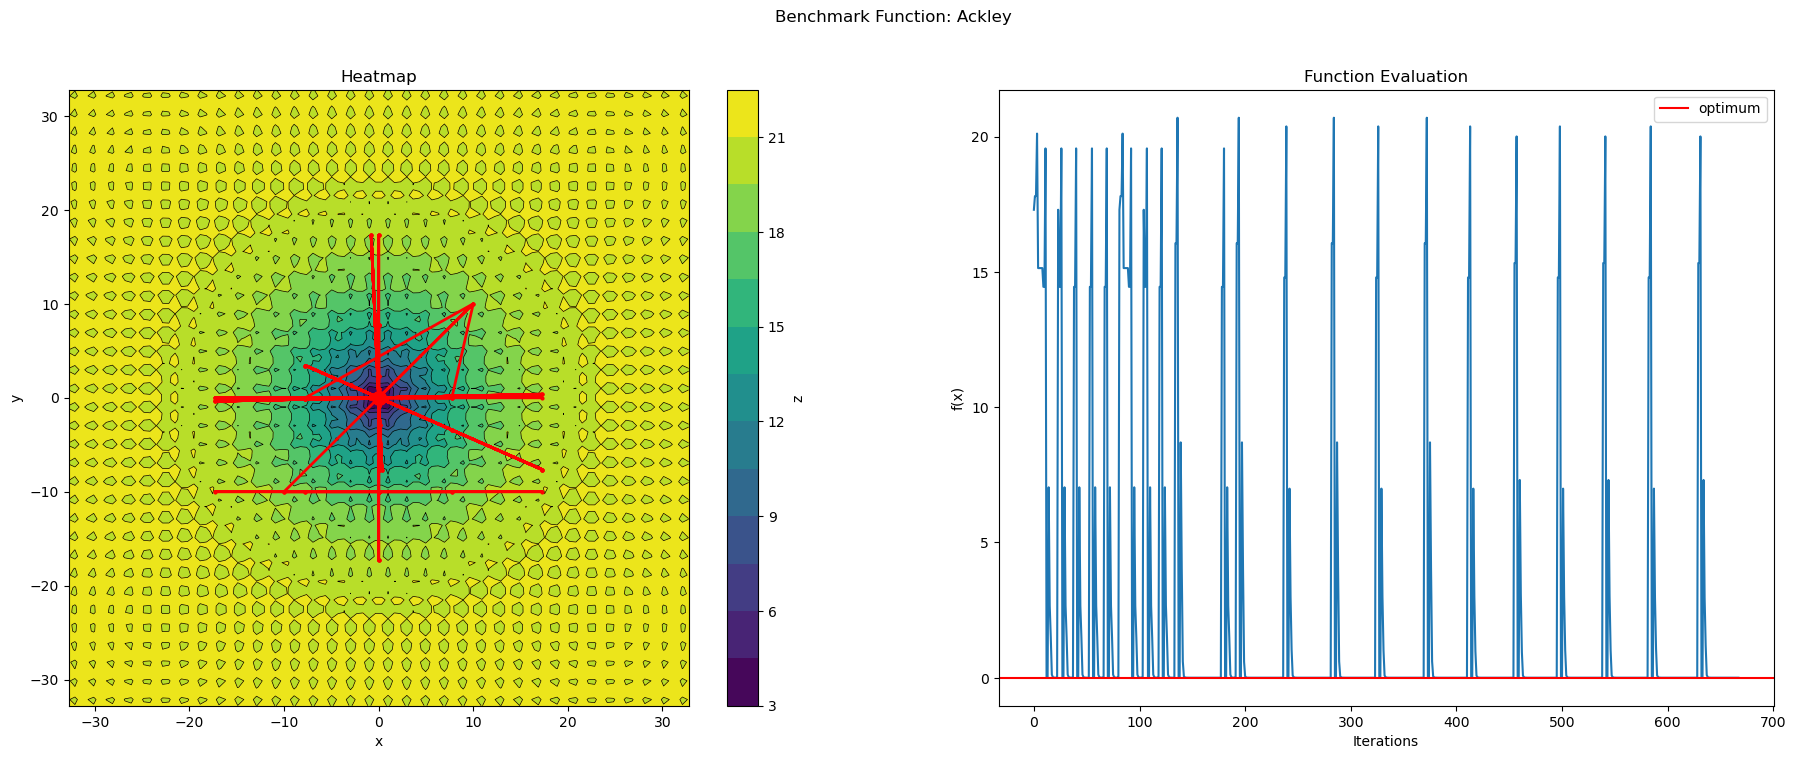
\includegraphics[width=\textwidth]{lab1/imgs/pw_ackley_opposite.png}
        \caption{Ackley with directions [-1,0],[0,-1]}
    \end{subfigure}
    \caption{Powell's method on the Ackley function with different initial directions}
    \label{fig:ackley}
\end{figure}

\subsection{Nelder-Mead}
\label{sec:nelder-mead}
Nelder-Mead is a direct search method that uses a simplex to perform the optimization. Compared to Powell, it's much more likely to get stuck in a local minimum and its performance is dependent on the choice of the initial point. For example below \ref{fig:nm-ackley} we can see the results of Nelder-Mead on the Ackley function where the method is able to converge to the global minimum with the right initial point but not with a different one.
\begin{figure}[H]
    \begin{subfigure}{0.5\textwidth}
        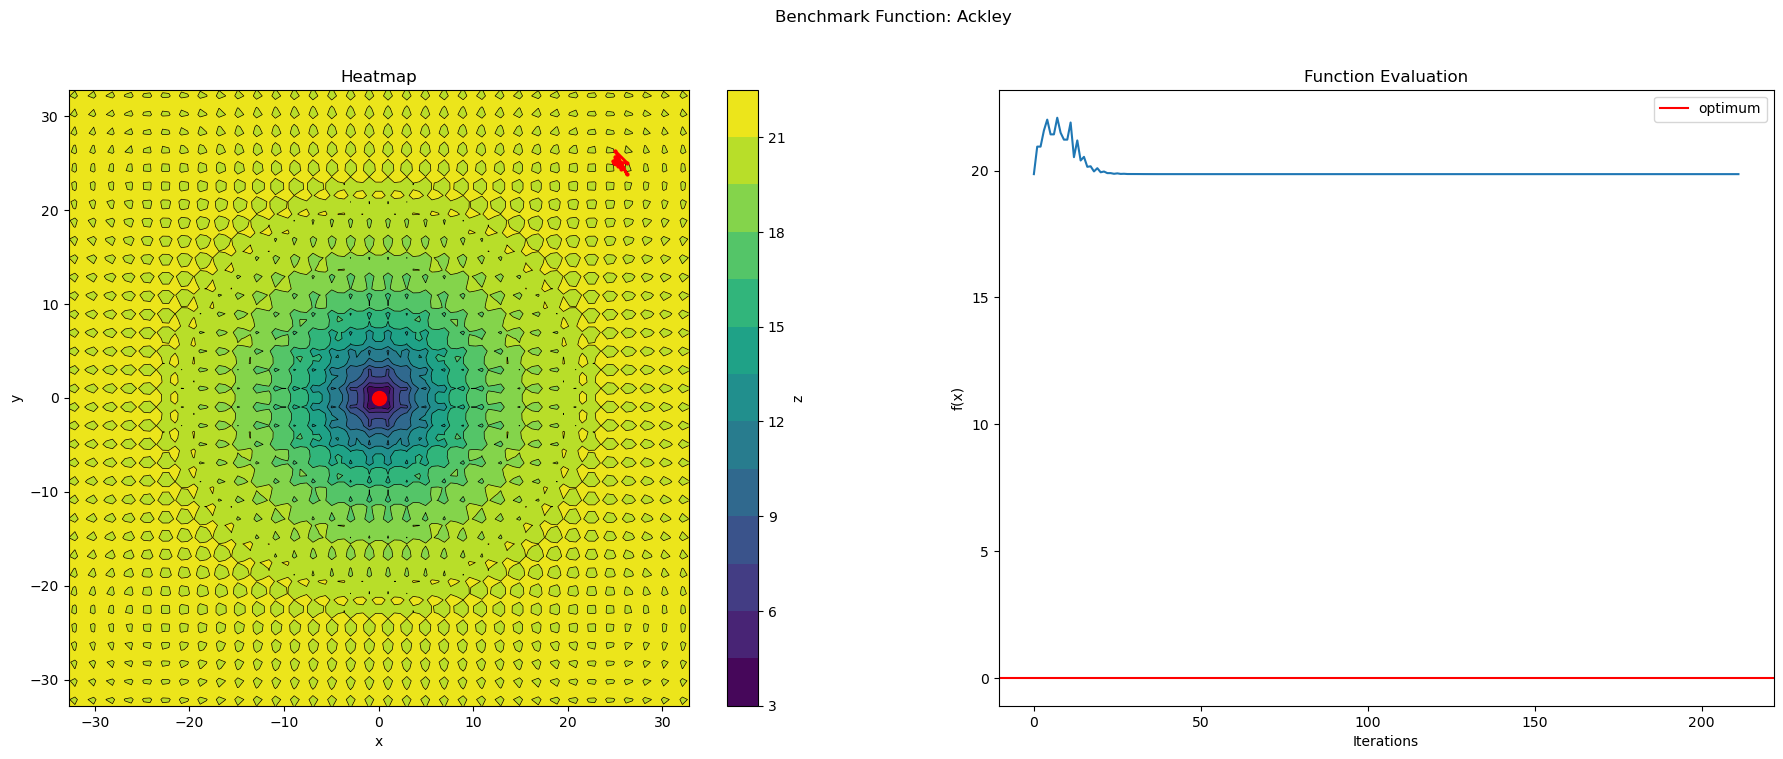
\includegraphics[width=\textwidth]{lab1/imgs/nm_ackley_20.png}
        \caption{Ackley with initial point [20,20]}
    \end{subfigure}
    \begin{subfigure}{0.5\textwidth}
        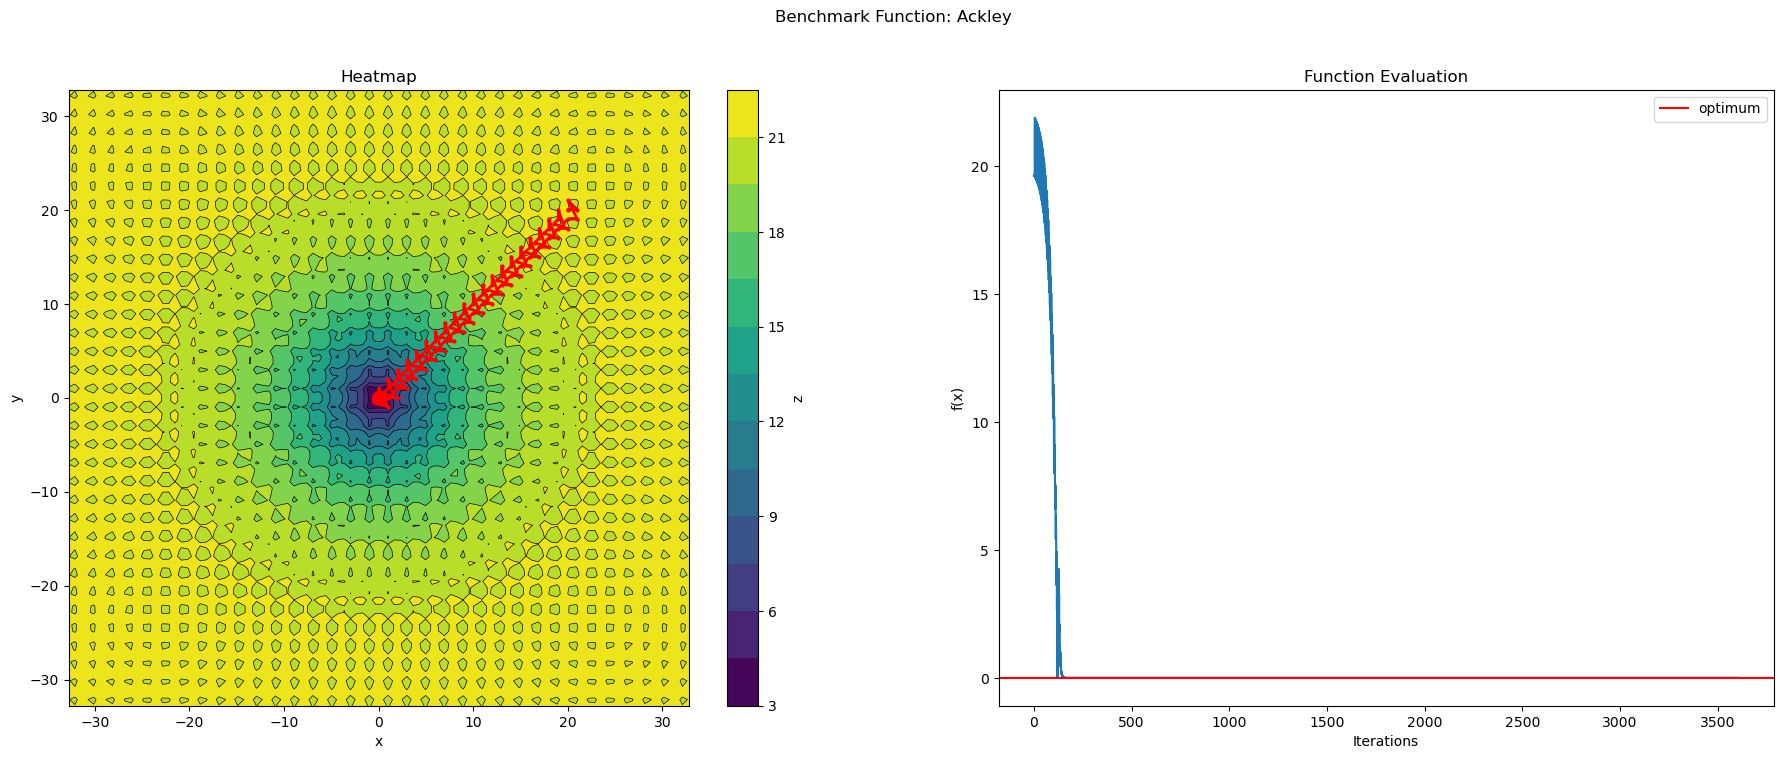
\includegraphics[width=\textwidth]{lab1/imgs/nm_ackley_25.png}
        \caption{Ackley with initial point [25,25]}
    \end{subfigure}
    \caption{Nelder-Mead on the Ackley function with different initial points}
    \label{fig:nm-ackley}
\end{figure}

Below \ref{fig:nm_rosenbrock} we can see the results of Nelder-Mead on the Rosenbrock function and we can see that the algorithms tends to obtain good results in unimodal functions with hard to approximate optima.
\begin{figure}[H]
    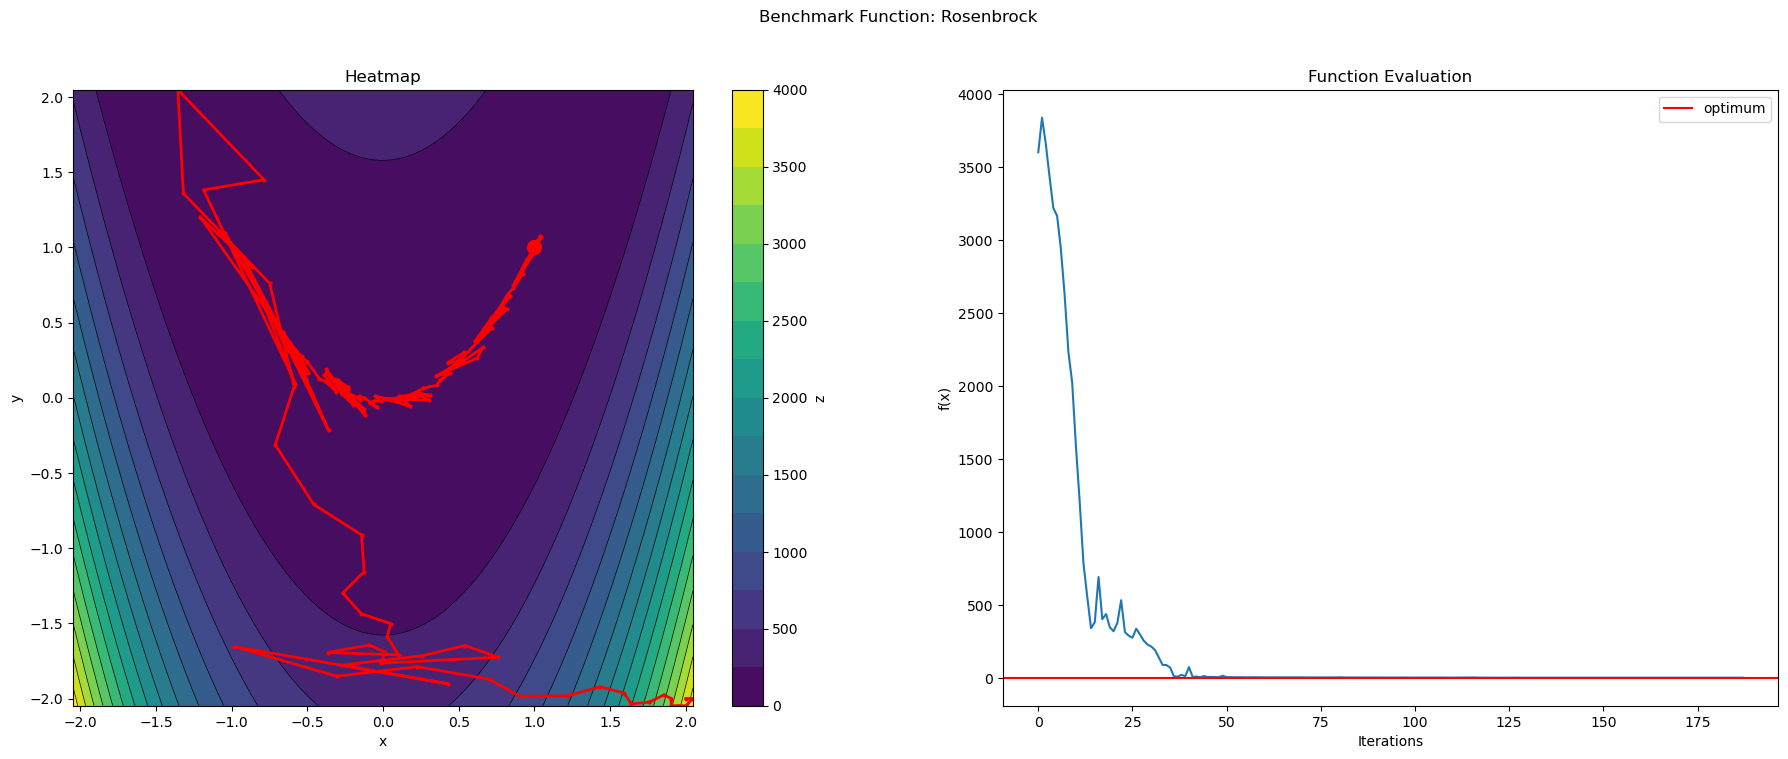
\includegraphics[width=\textwidth]{lab1/imgs/nm_rosenbrock.png}
    \caption{Nelder-Mead on the Rosenbrock function}
    \label{fig:nm_rosenbrock}
\end{figure}
Even on the functions where the method performs well, the number of iterations required is quite high. For example, below \ref{fig:hypersphere-100} we compare the results of the Nelder-Mead and the Powell algorithm on the Hypersphere function, both with 10 iterations.
\begin{figure}[H]
    \begin{subfigure}{0.5\textwidth}
        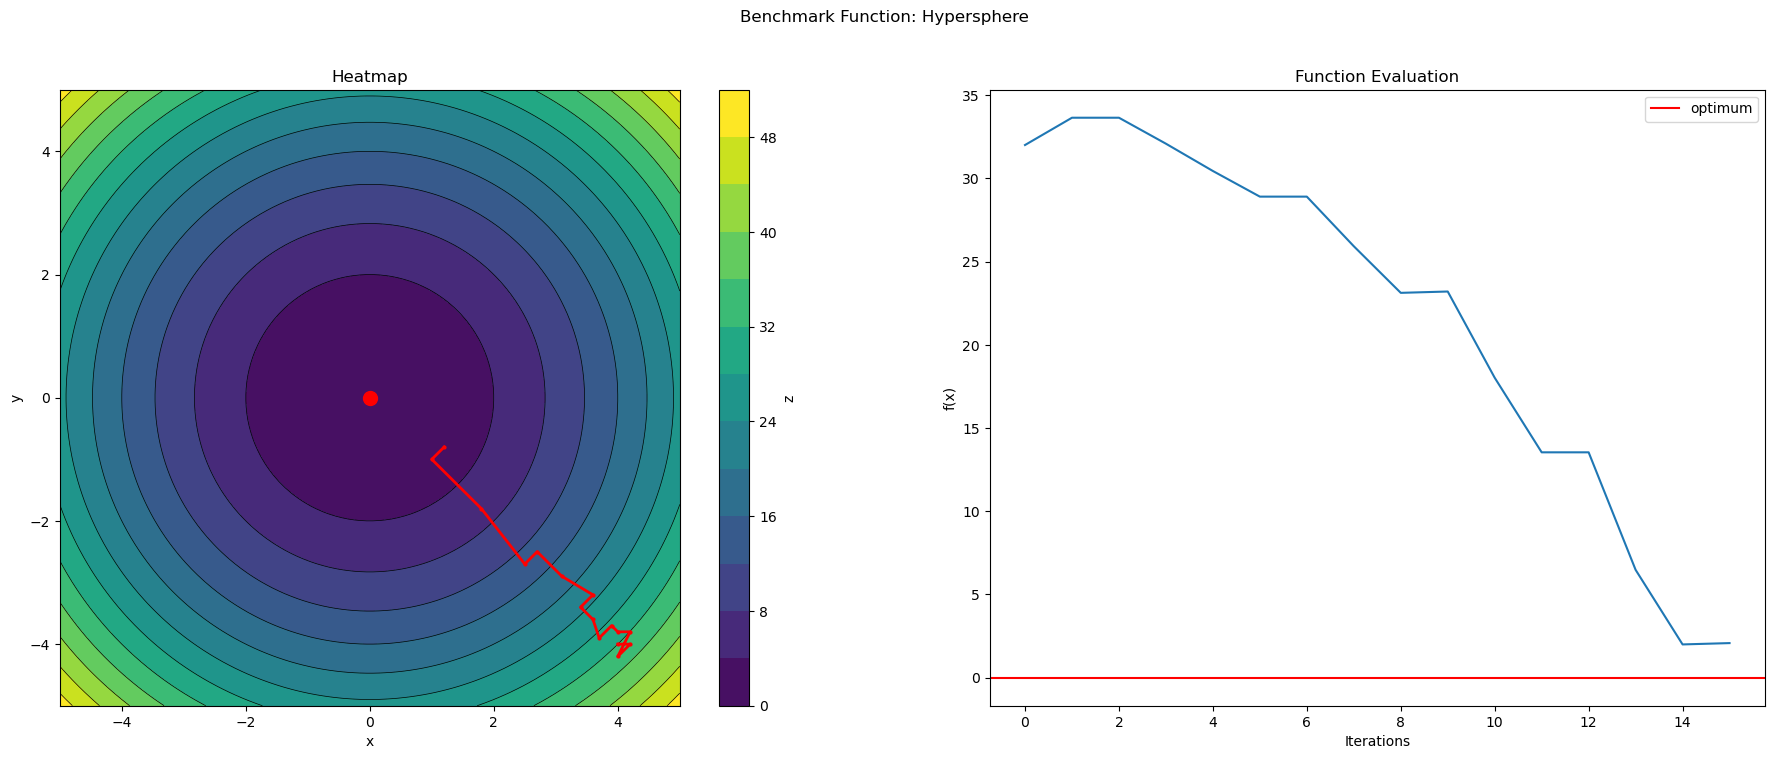
\includegraphics[width=\textwidth]{lab1/imgs/nm_hypersphere_100_iter.png}
        \caption{Nelder-Mead with 10 iterations}
    \end{subfigure}
    \begin{subfigure}{0.5\textwidth}
        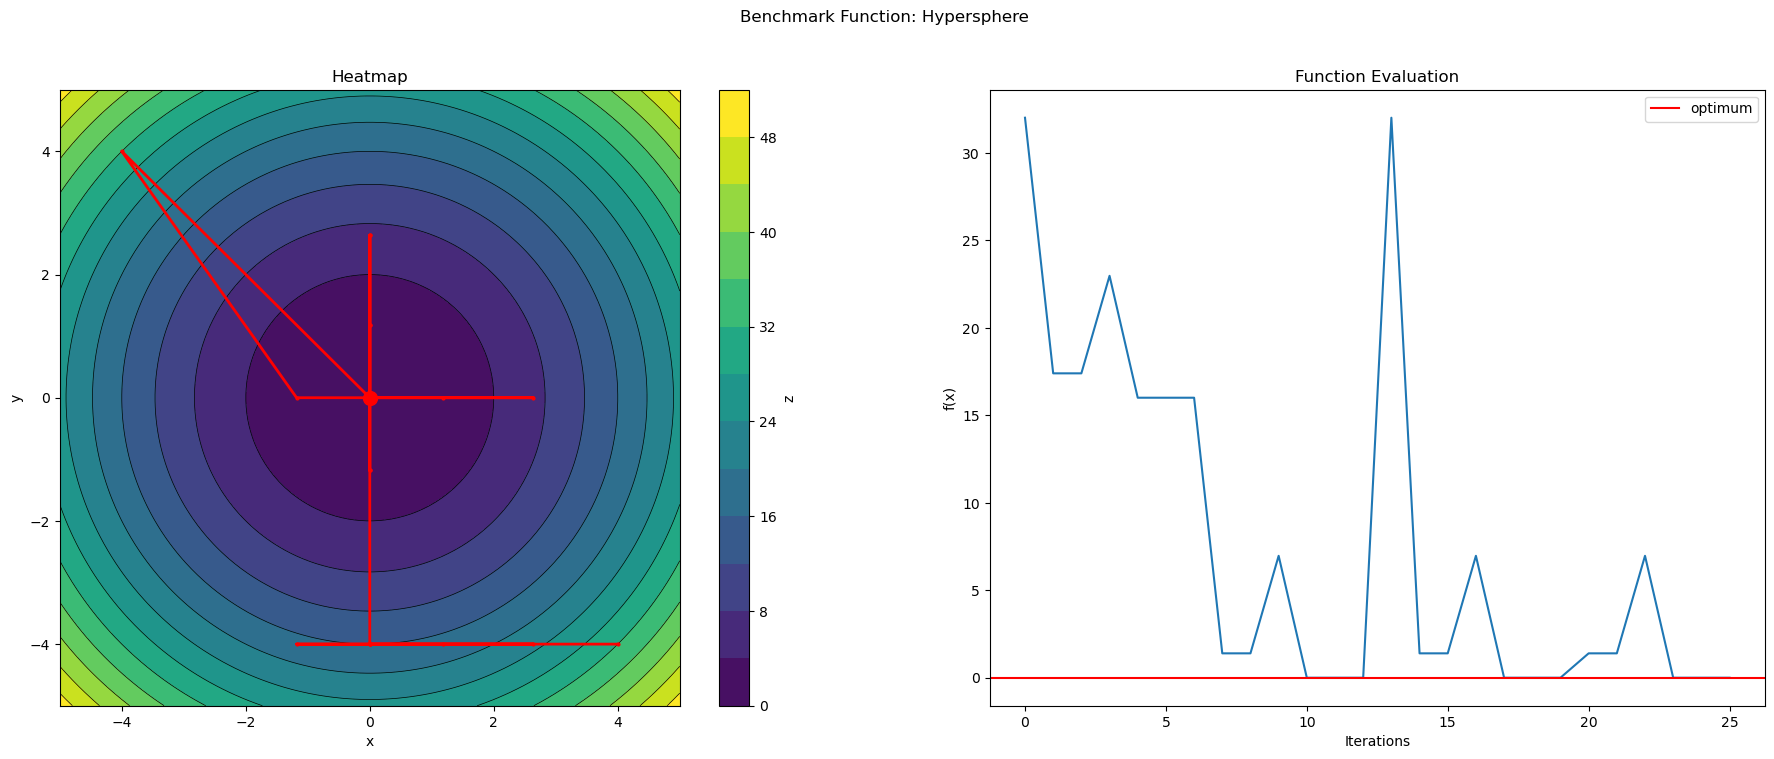
\includegraphics[width=\textwidth]{lab1/imgs/pw_hypersphere_10_iter.png}
        \caption{Powell with 10 iterations}
    \end{subfigure}
    \caption{Nelder-Mead and Powell on the Hypersphere function with 10 iterations}
    \label{fig:hypersphere-100}
\end{figure}
We can see how different methods perform differently on different functions. This is also supported by the No Free Lunch Theorem which states that no optimization algorithm is better than any other when their performance is averaged over all possible functions. This means that the choice of the optimization algorithm is dependent on the specific problem at hand.
\newpage

\section{DIRECT, Basing Hopping}
\subsection{DIRECT}
DIviding RECTangles (DIRECT) is a partitioning algorithm that recursively subdivides the feasible region into smaller hyperrectangles. The algorithm is as follows:
\begin{enumerate}
    \item Divide the feasible region into smaller hyperrectangles.
    \item Evaluate the function at the center of each hyperrectangle. The division is performed so that the region with the best function value is given the largest space.
    \item a set of potentially optimal hyperrectangles is identified and further divided.
\end{enumerate}
The stopping condition is either based on the maximum number of iterations / function evaluations or on the improvemnt of the function value. This means that the specific tolerance is dependent on the problem being solved. For example in the case of the De Jong's function \ref{fig:dejong-tolerance} we can see that different tollerance levels lead to different results.
\begin{figure}[H]
    \begin{subfigure}{0.5\textwidth}
        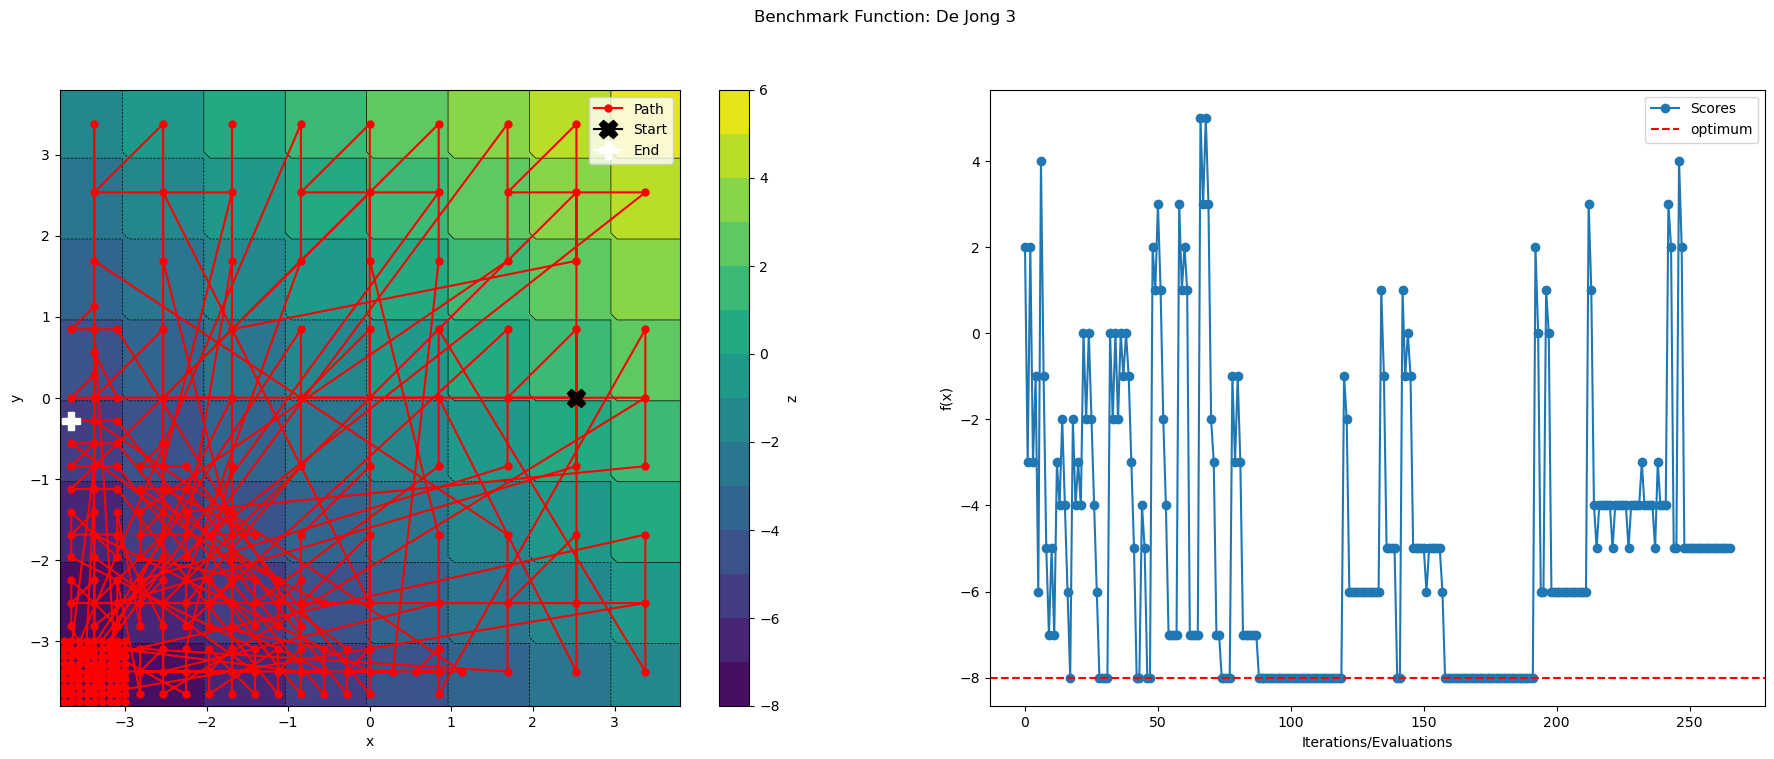
\includegraphics[width=\textwidth]{lab2/imgs/di_dejong_eps_01.png}
        \caption{$\epsilon =0.1$}
    \end{subfigure}
    \begin{subfigure}{0.5\textwidth}
        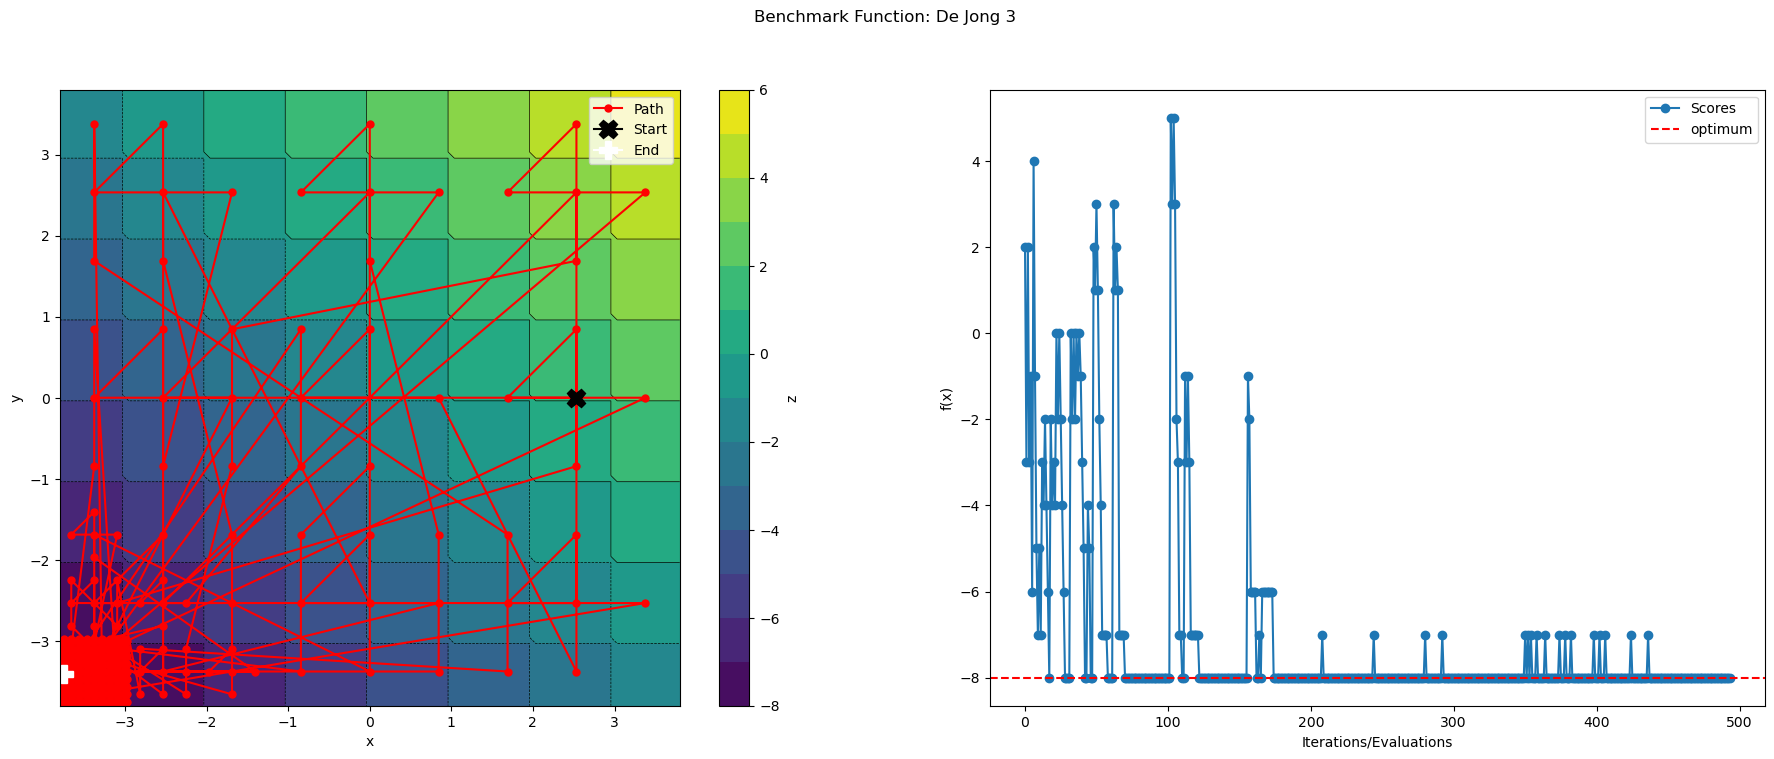
\includegraphics[width=\textwidth]{lab2/imgs/di_dejong_eps_001.png}
        \caption{$\epsilon =0.001$}
    \end{subfigure}
    \caption{DIRECT on De Jong's function with different tolerances}
    \label{fig:dejong-tolerance}
\end{figure}
For other functions, such as the Ackley function, the tolerance level does not have an impact on the results, probably bacause the function has a more clear basin of attraction towards the global minimum.
\begin{figure}[H]
    \begin{subfigure}{0.5\textwidth}
        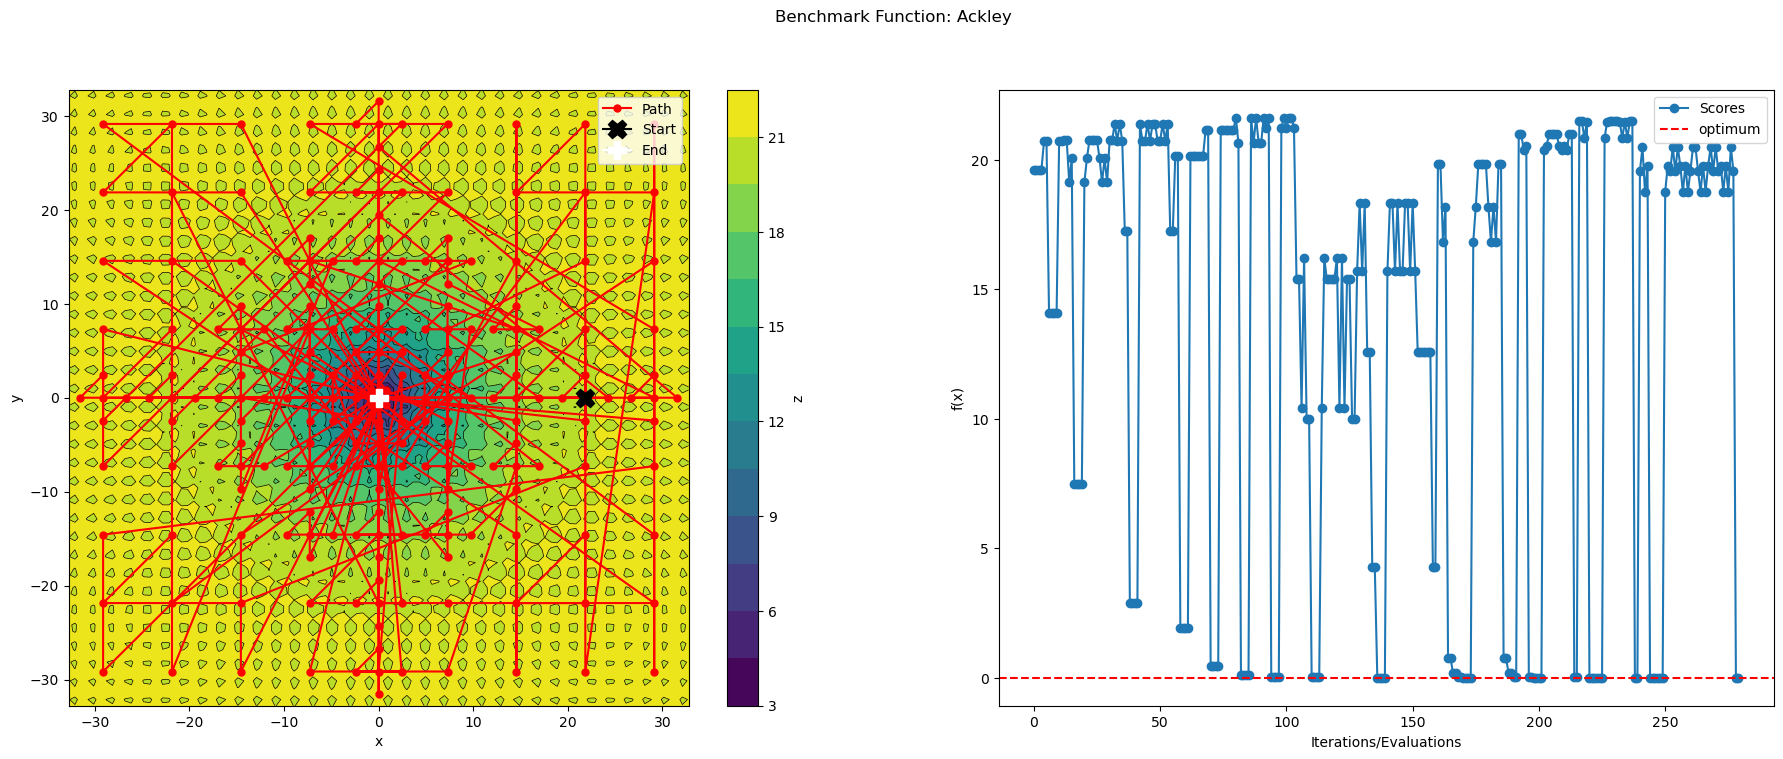
\includegraphics[width=\textwidth]{lab2/imgs/di_ackley_eps_01.png}
        \caption{$\epsilon =0.1$}
    \end{subfigure}
    \begin{subfigure}{0.5\textwidth}
        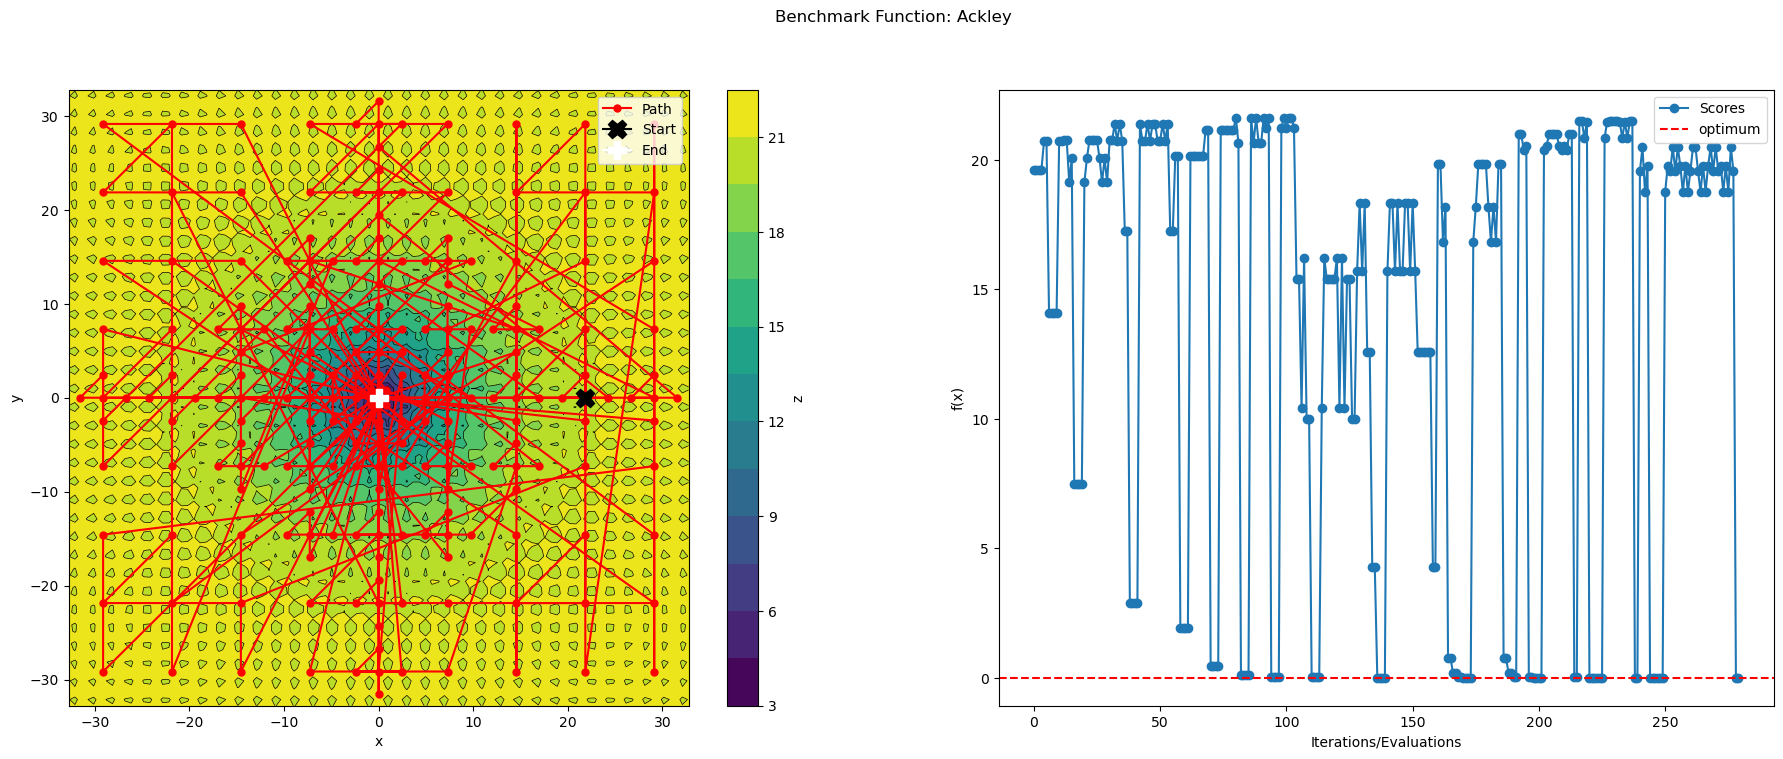
\includegraphics[width=\textwidth]{lab2/imgs/di_ackley_eps_001.png}
        \caption{$\epsilon =0.001$}
    \end{subfigure}
    \caption{DIRECT on Ackley's function with different tolerances}
    \label{fig:ackley-tolerance}
\end{figure}

As we would expect, a larger number of iterations leads to a better approximation of the global minimum, in some more extreme cases even changing the basin of attraction of the global minimum. This is the case for the De Jong's function \ref{fig:dejong-iterations} where the minimum found is significantly different for different numbers of evaluations.
\begin{figure}[H]
    \begin{subfigure}{0.5\textwidth}
        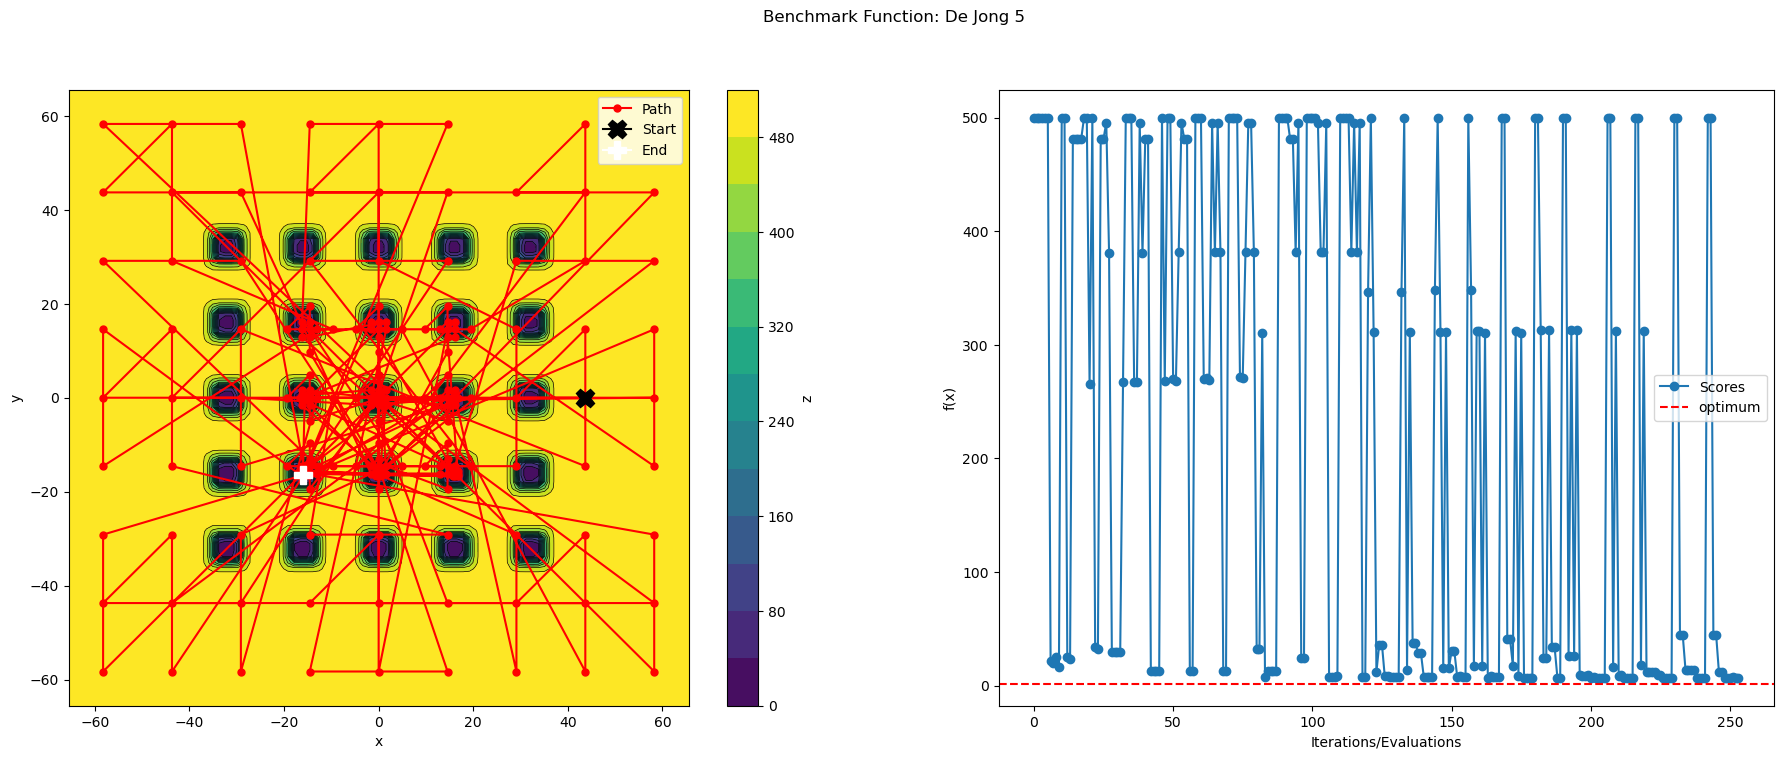
\includegraphics[width=\textwidth]{lab2/imgs/di_i100_e250.png}
        \caption{100 iterations and 250 evaluations}
    \end{subfigure}
    \begin{subfigure}{0.5\textwidth}
        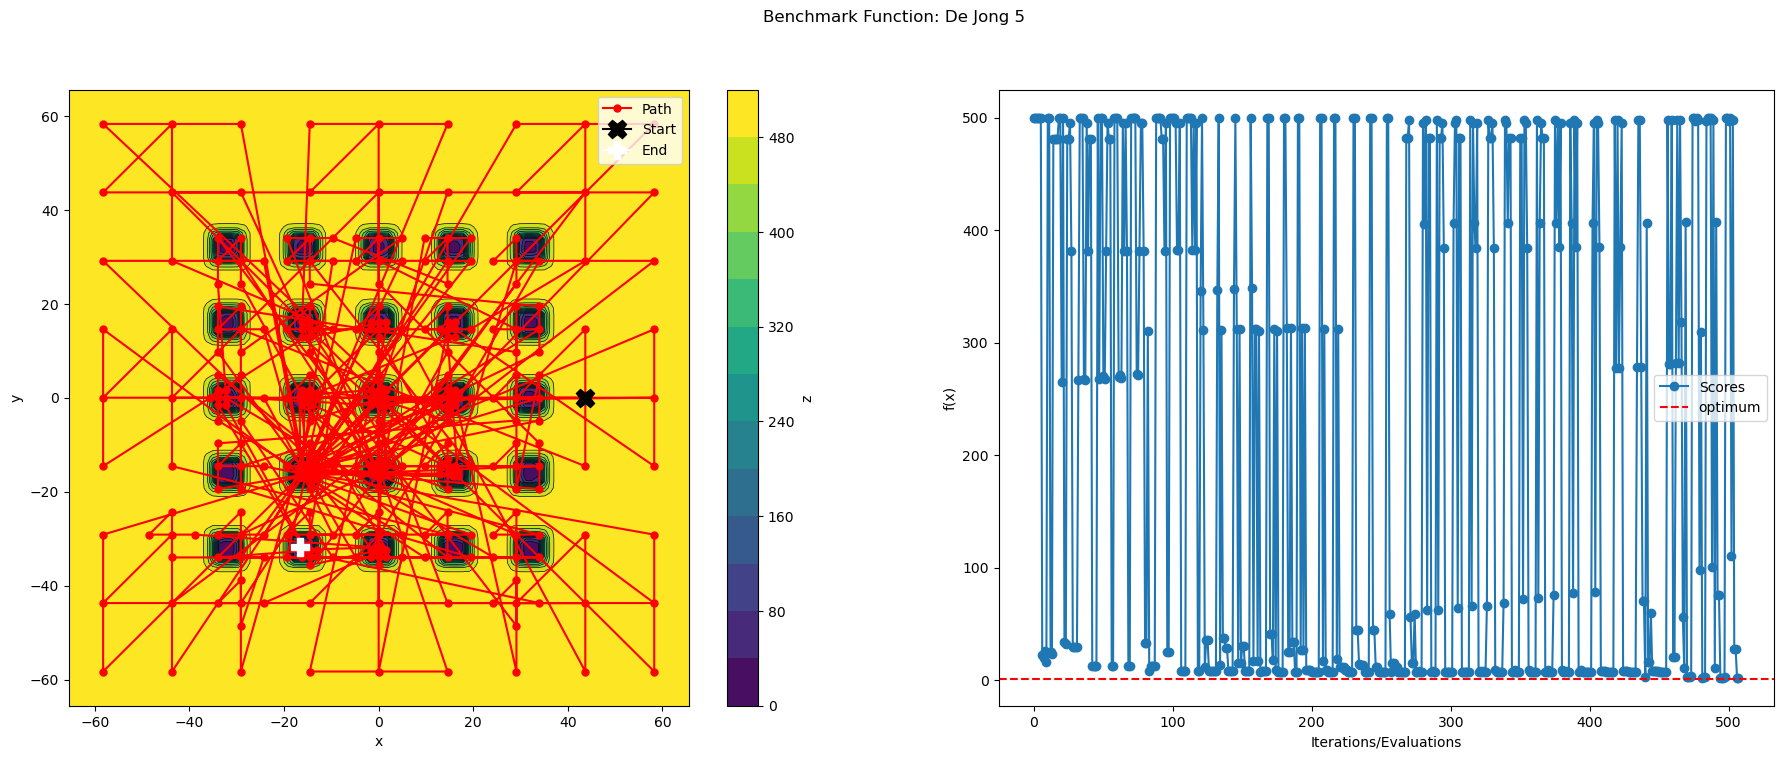
\includegraphics[width=\textwidth]{lab2/imgs/di_i100_e500.png}
        \caption{100 iterations and 500 evaluations}
    \end{subfigure}\\
    \begin{subfigure}{\textwidth}
        \centering
        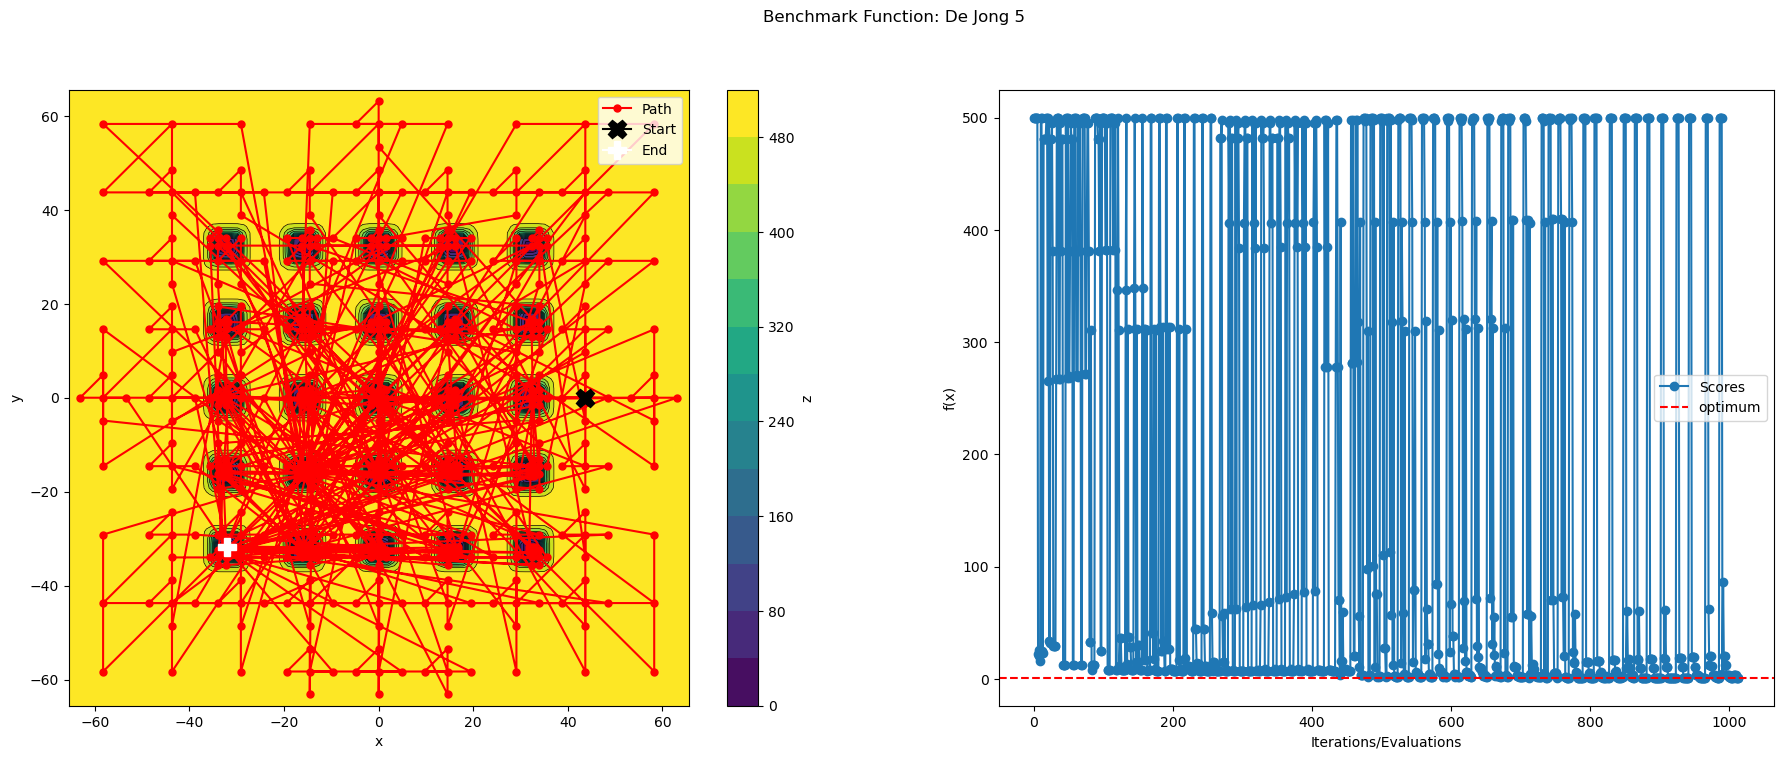
\includegraphics[width=0.5\textwidth]{lab2/imgs/di_i100_e1000.png}
        \caption{100 iterations and 1000 evaluations}
    \end{subfigure}
    \caption{DIRECT on De Jong's function with different number of evaluations}
    \label{fig:dejong-iterations}
\end{figure}

Another interesting thing to note is the behaviour of the algorithm with a large number of local minima and how we can see how DIRECT evaluations are much more spread out compared to other functions. This can be seen really well in the Griewank function \ref{fig:griewank}.
\begin{figure}[H]
    \centering
    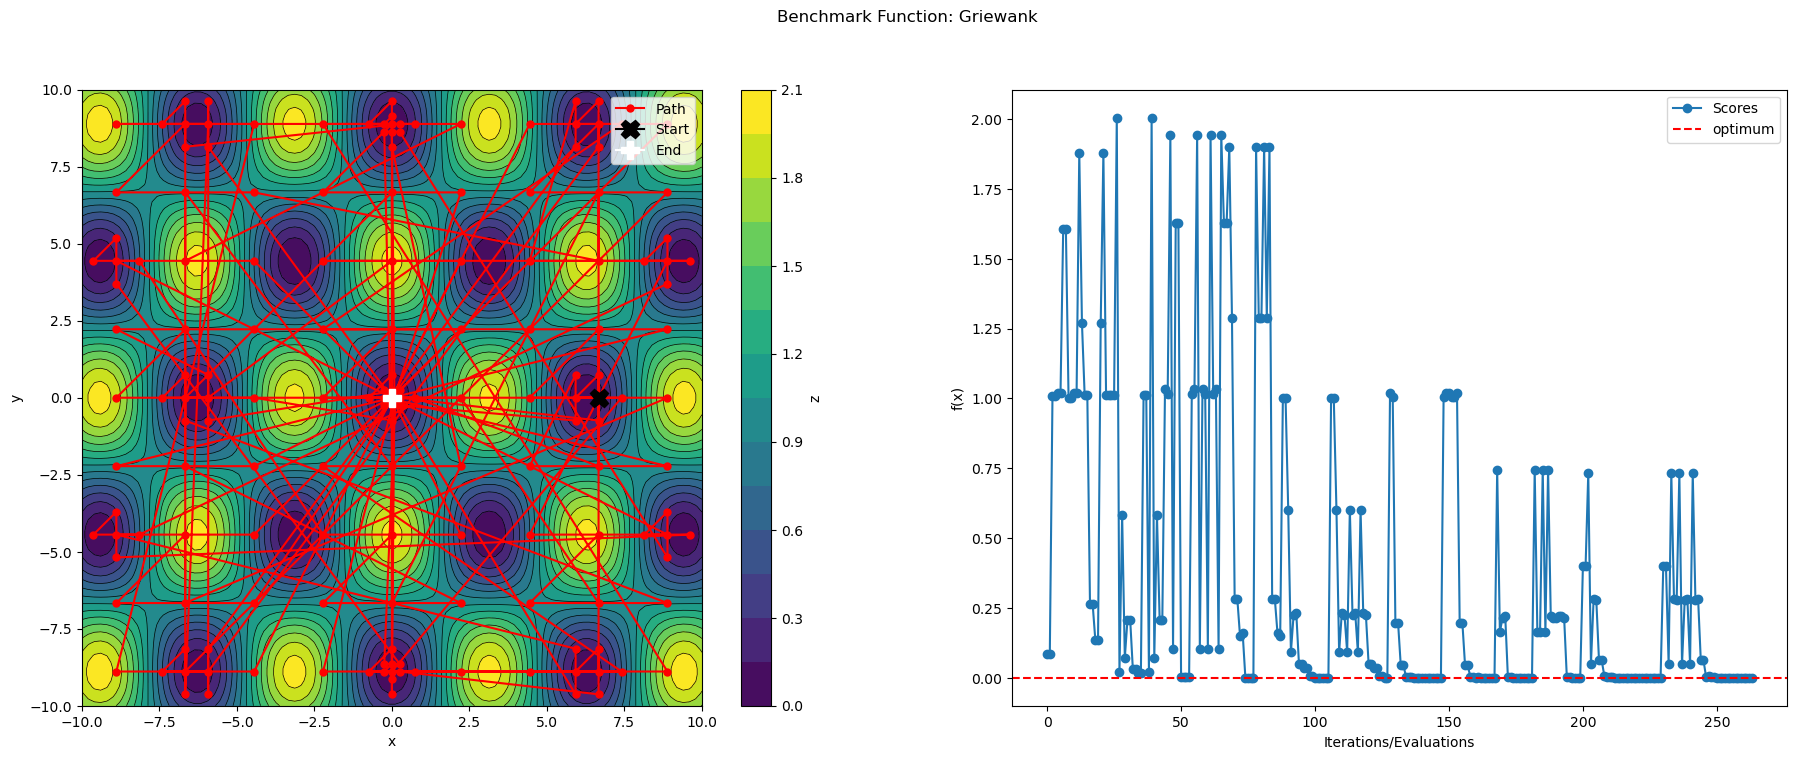
\includegraphics[width=0.8\textwidth]{lab2/imgs/griewank.png}
    \caption{DIRECT on Griewank's function}
    \label{fig:griewank}
\end{figure}

\subsection{Basin Hopping}
Basing Hopping is a form of Iterated Local Search with a different starting point each time. It loops through the following steps:
\begin{enumerate}
    \item \textit{Hopping}: perturbation of the current solution ("jump" to new parts of the search space)
    \item \textit{Local Search}: perturbed solution is optimized using a local search method
    \item \textit{Acceptance} the new solution is accepted or rejected based on an acceptance criterion. This criterion can be defined in different ways; here is defined based on the Metropolis criterion.
\end{enumerate}
It's particularly important to set the temperature and the stepsize parameters correctly as specified in the scipy documentation. In particular:
\begin{enumerate}
    \item \textit{Temperature}: usually set to be comparable with with the separation of the objective function value of local minima.
    \item \textit{Stepsize}: should be set to be comparable to the Distance in the coordinates between local minima.
\end{enumerate}

For example, we can see how the algorithm behaves with the Dejong5 function \ref{fig:bh-dejong} with different temperatures (10 and 0.1) and that the temperature has a significant impact on the evaluations: The higher temperature leads to a more spread out evaluation of the function because the algorithm is more likely to accept worse solutions and leave the local basin of attraction.
\begin{figure}[H]
    \begin{subfigure}{0.5\textwidth}
        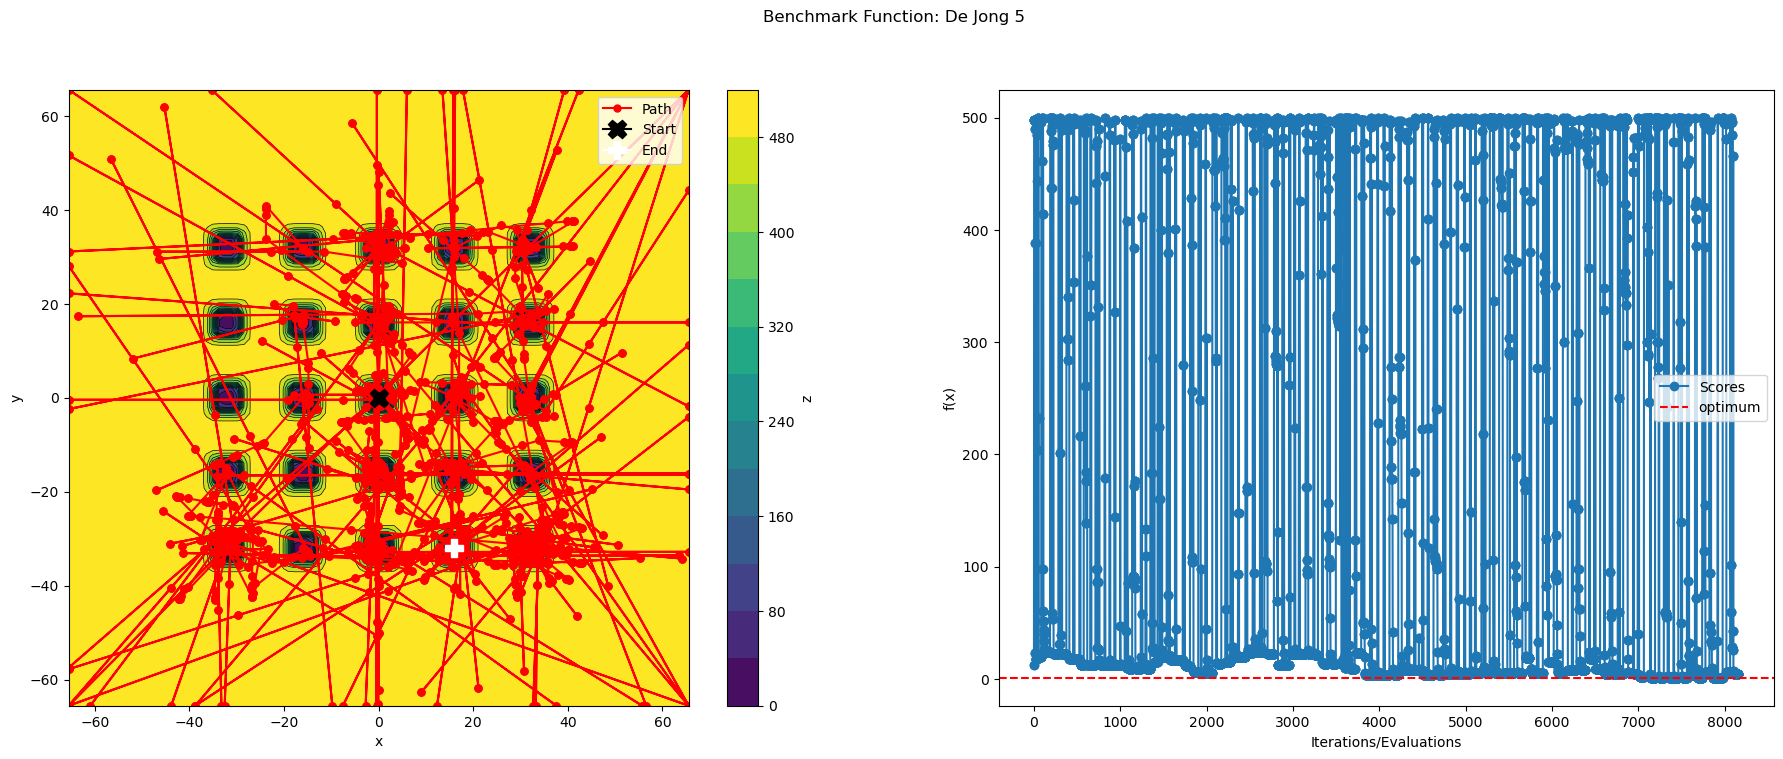
\includegraphics[width=\textwidth]{lab2/imgs/bh_dejong_10.png}
        \caption{Temperature = 10}
    \end{subfigure}
    \begin{subfigure}{0.5\textwidth}
        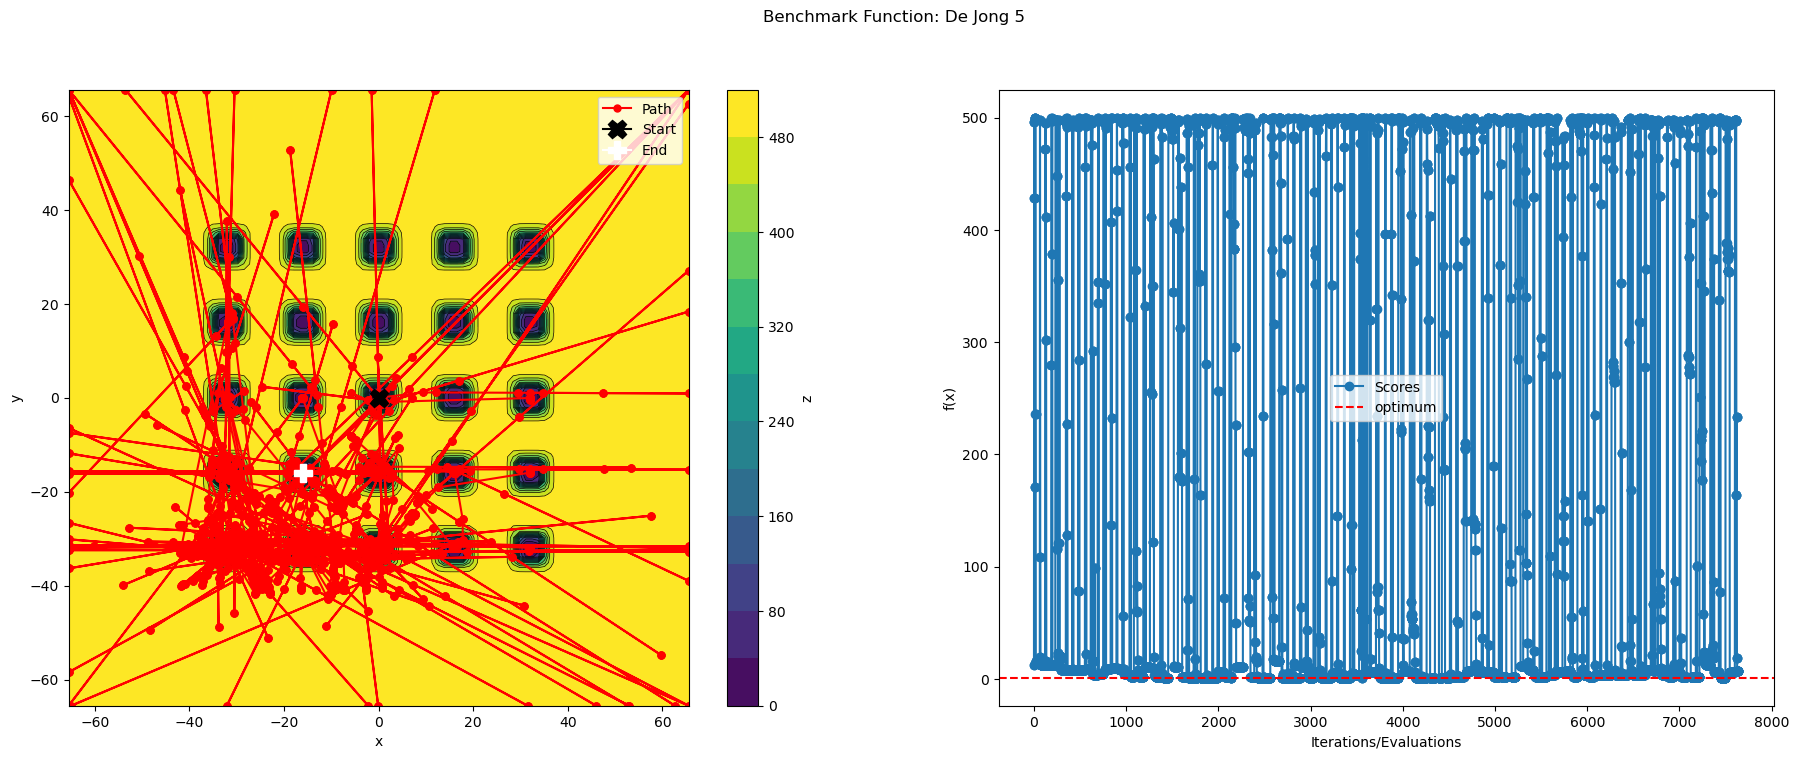
\includegraphics[width=\textwidth]{lab2/imgs/bh_dejong_01.png}
        \caption{Temperature = 0.1}
    \end{subfigure}
    \caption{Basin Hopping on De Jong's function with different temperatures and stepsize 20}
    \label{fig:bh-dejong}
\end{figure}
The importance of the stepsize can be seen by comparing the previous results with the ones obtained with a stepsize of 1 (Figure \ref{fig:bh-dejong-stepsize}) where we can clearly see that the algorithm isn't able to leave the local basin of attraction.
\begin{figure}[H]
    \centering
    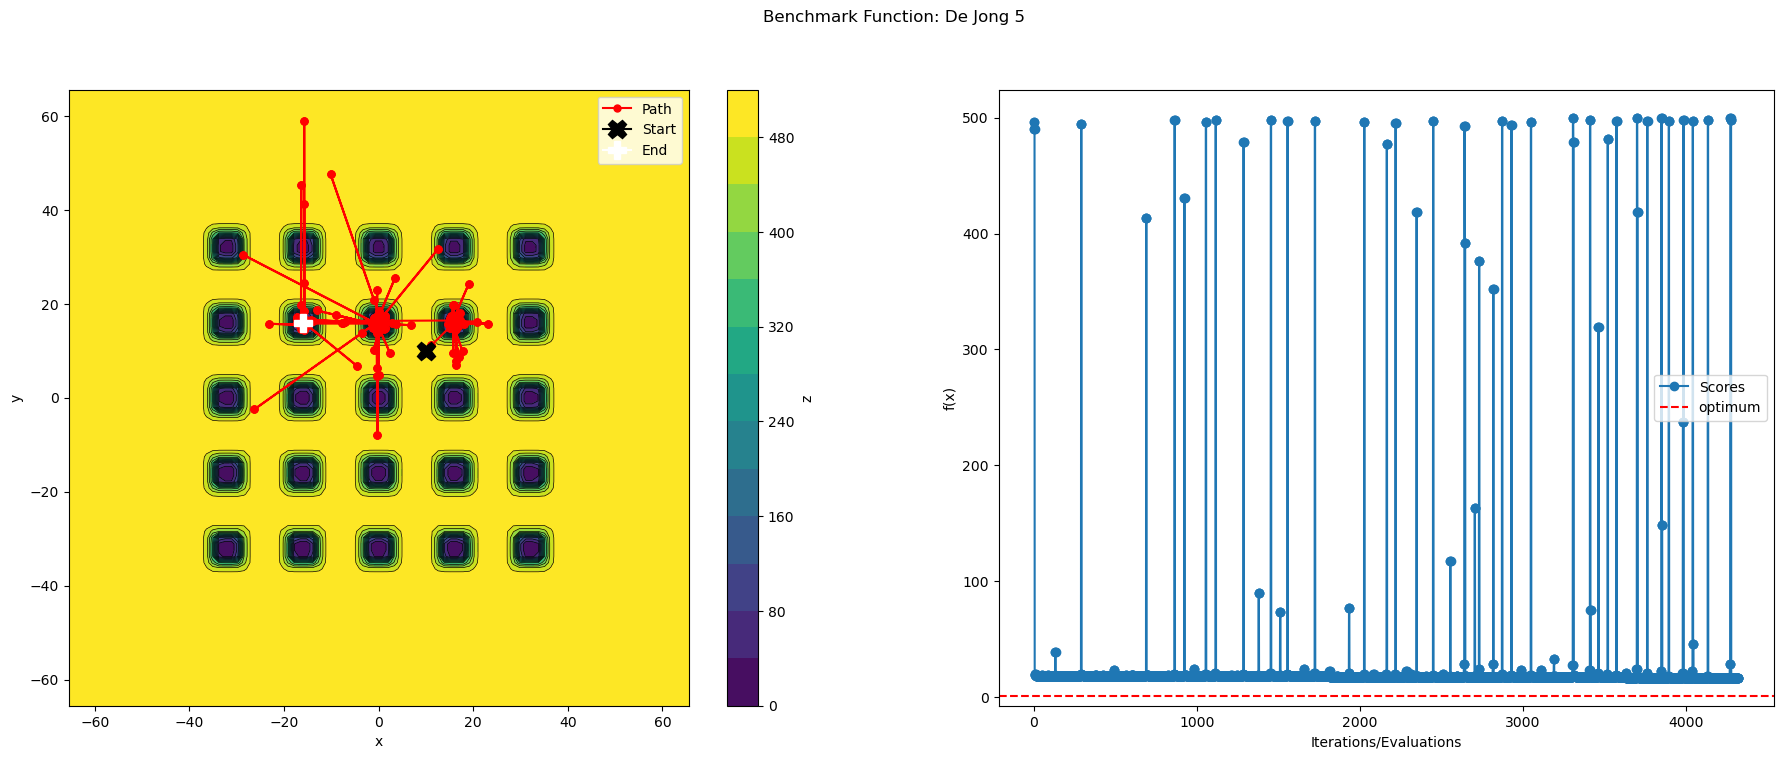
\includegraphics[width=0.8\textwidth]{lab2/imgs/bh_dejong_step_1.png}
    \caption{Basin Hopping on De Jong's function with stepsize = 1}
    \label{fig:bh-dejong-stepsize}
\end{figure}

It's also interesting to note that, even if the global minimum is found, this isn't necessarily the last evaluation of the function. This makes sense because the only stopping condition is the number of iterations, so the algorithm will continue to evaluate the function even after finding the global minimum. 

If we have a unimodal function, such as the Rosenbrock function \ref*{fig:bh-rosenbrock}, the algorithm is able to immediately find the global minimum via the local search step.
\begin{figure}[H]
    \centering
    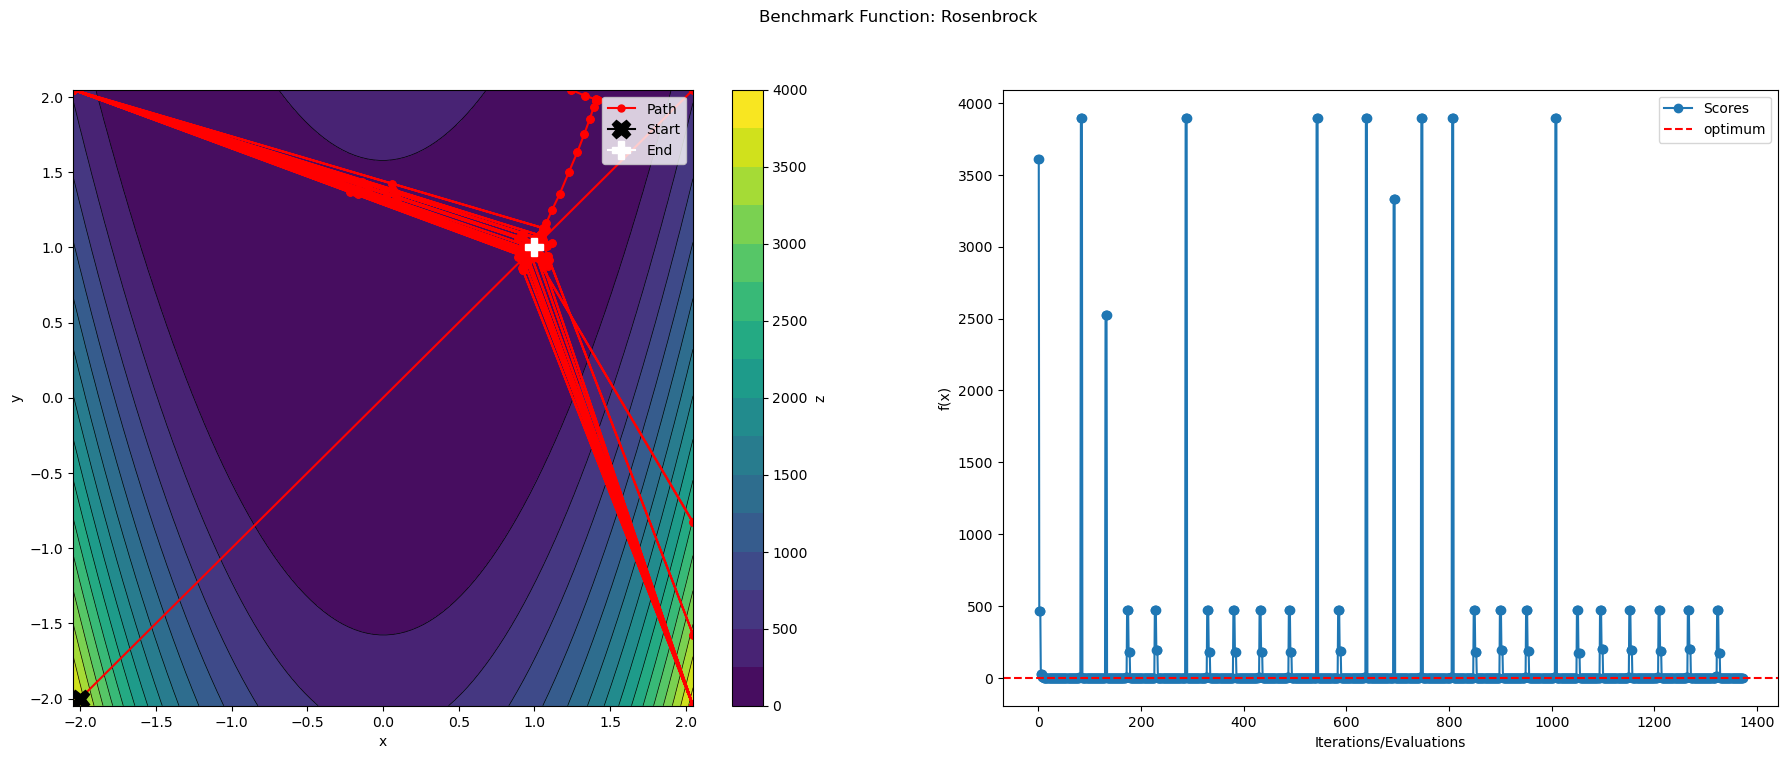
\includegraphics[width=0.8\textwidth]{lab2/imgs/bh_rosenbrock.png}
    \caption{Basin Hopping on Rosenbrock's function}
    \label{fig:bh-rosenbrock}
\end{figure}

\noindent
\textbf{Note}: the code was slightly modified to add bounds to the local search algorithm (L-BFGS-B) to avoid the algorithm from going out of bounds.


\newpage

\section{Derivative Based Optimization}
\subsection{Gradient Descent}
\label{sec:gradient-descent}
Gradient descent is a first order optimization method, which means that it uses the first derivative of the function to find the minimum. The algorithm works by taking steps in the opposite direction of the gradient of the function, which is the direction of the steepest descent. The step size is controlled by the learning rate, which is a hyperparameter.

If the learning rate is too big then the gradient descent can overshoot the minimum and only then adjust to convergence. If the learning rate is too small then the gradient will take more iterations to converge but for convex functions the gradient descent will always converge at some point given enough steps \ref{fig:gd-hypersphere}.

\begin{figure}[H]
    \begin{subfigure}{0.5\linewidth}
        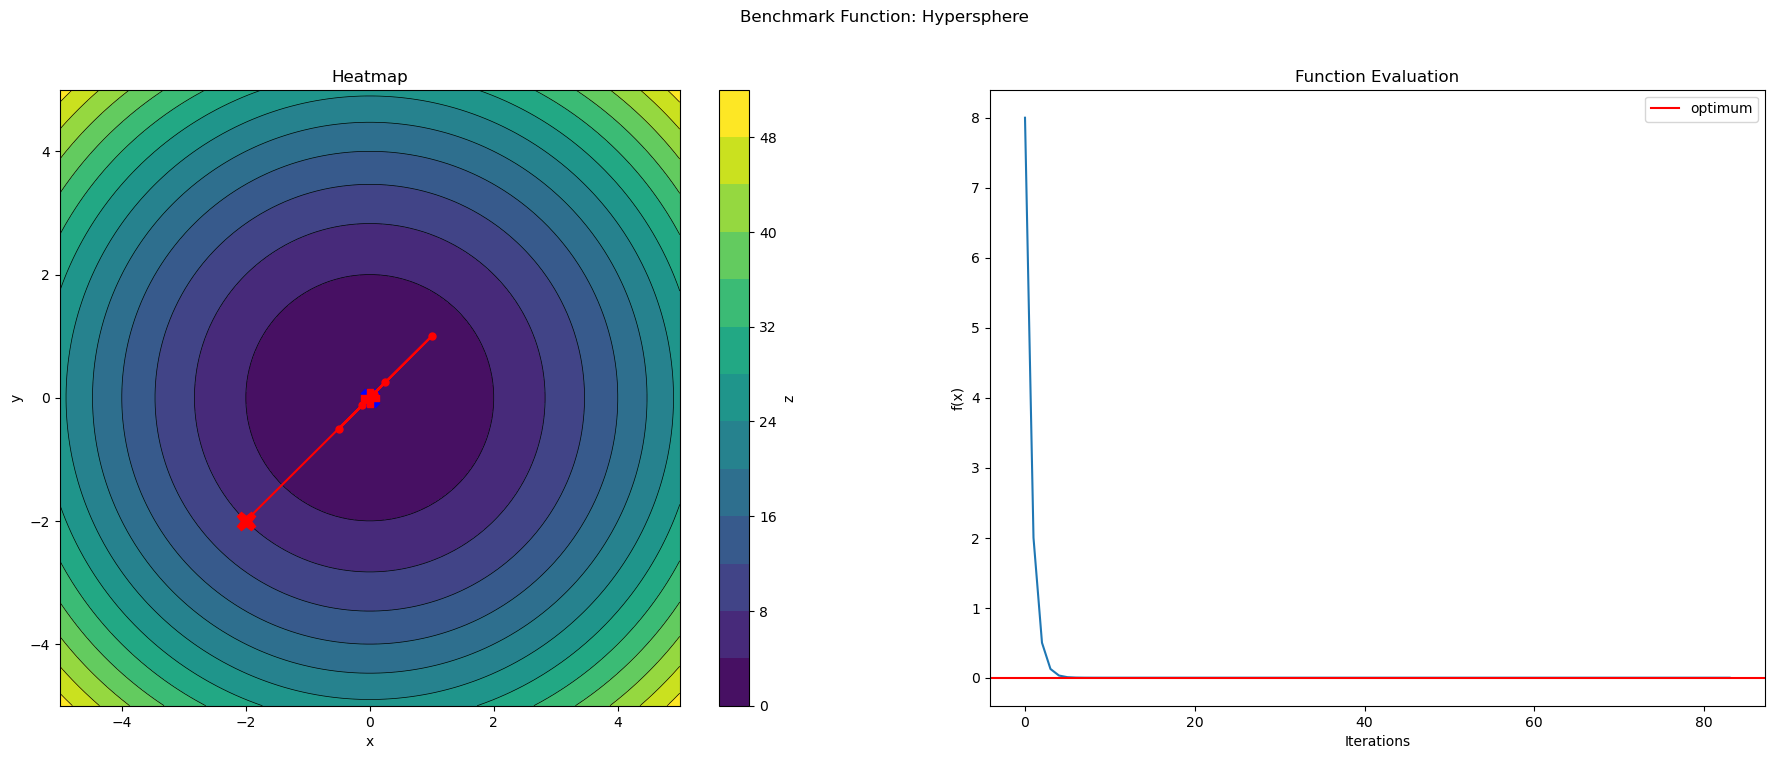
\includegraphics[width=\linewidth]{lab3/imgs/gd_sphere_75.png}
        \caption{Gradient descent with learning rate 0.75}
    \end{subfigure}
    \begin{subfigure}{0.5\linewidth}
        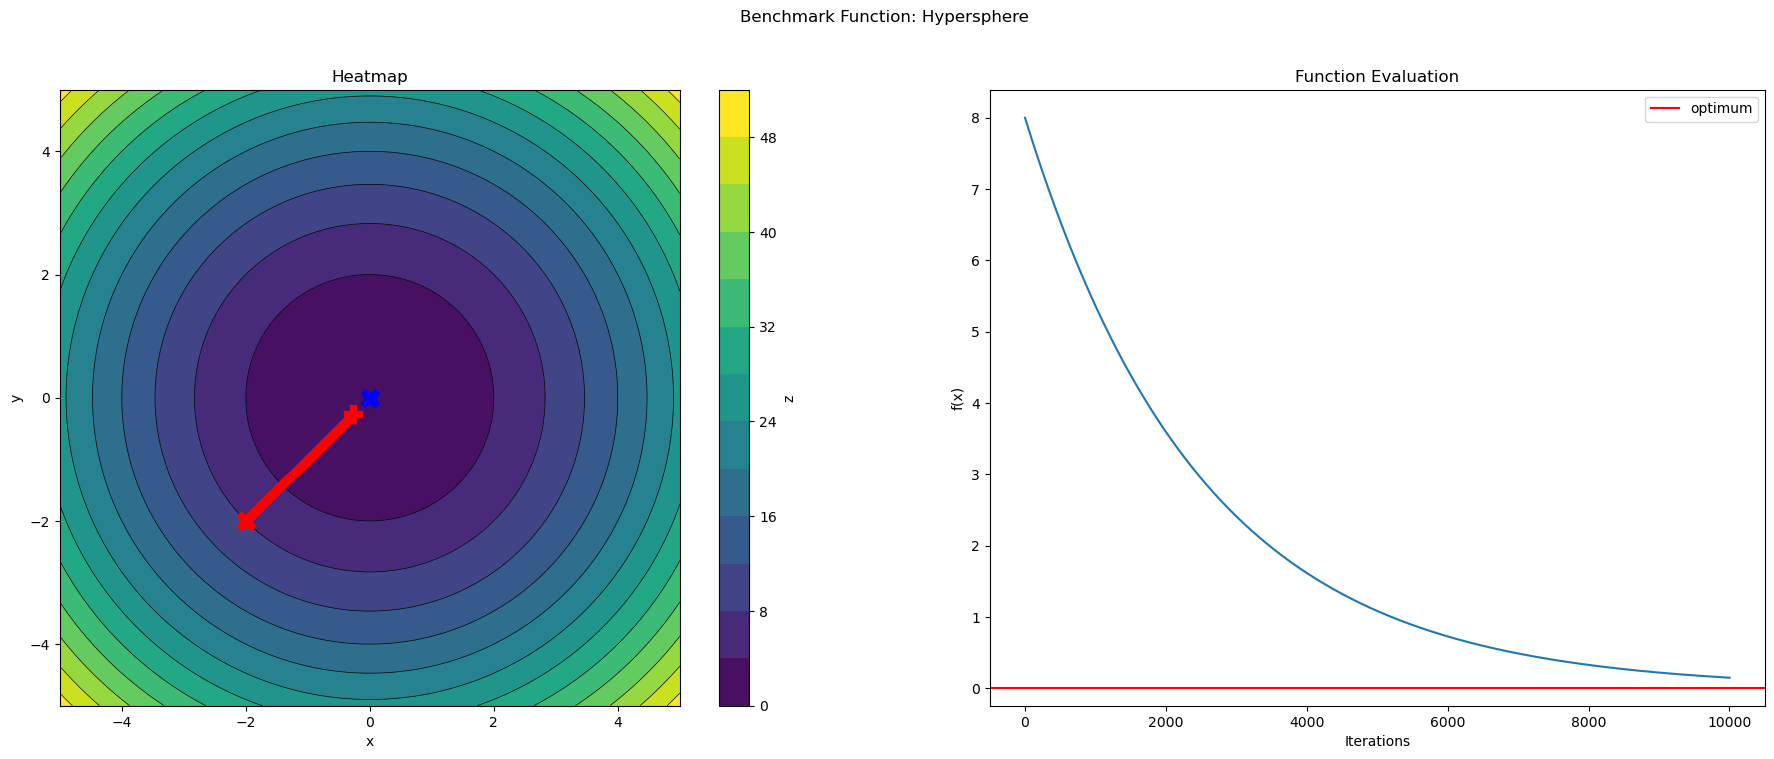
\includegraphics[width=\linewidth]{lab3/imgs/gd_sphere_04.png}
        \caption{Gradient descent with learning rate 0.4}
    \end{subfigure}
    \caption{Gradient descent on a 2D hypersphere}
    \label{fig:gd-hypersphere}
\end{figure}

For multimodal functions (many local minima), the gradient descent is only guaranteed to converge to the nearest local minimum, thus the starting point is very important.
\begin{figure}[H]
    \begin{subfigure}{0.5\linewidth}
        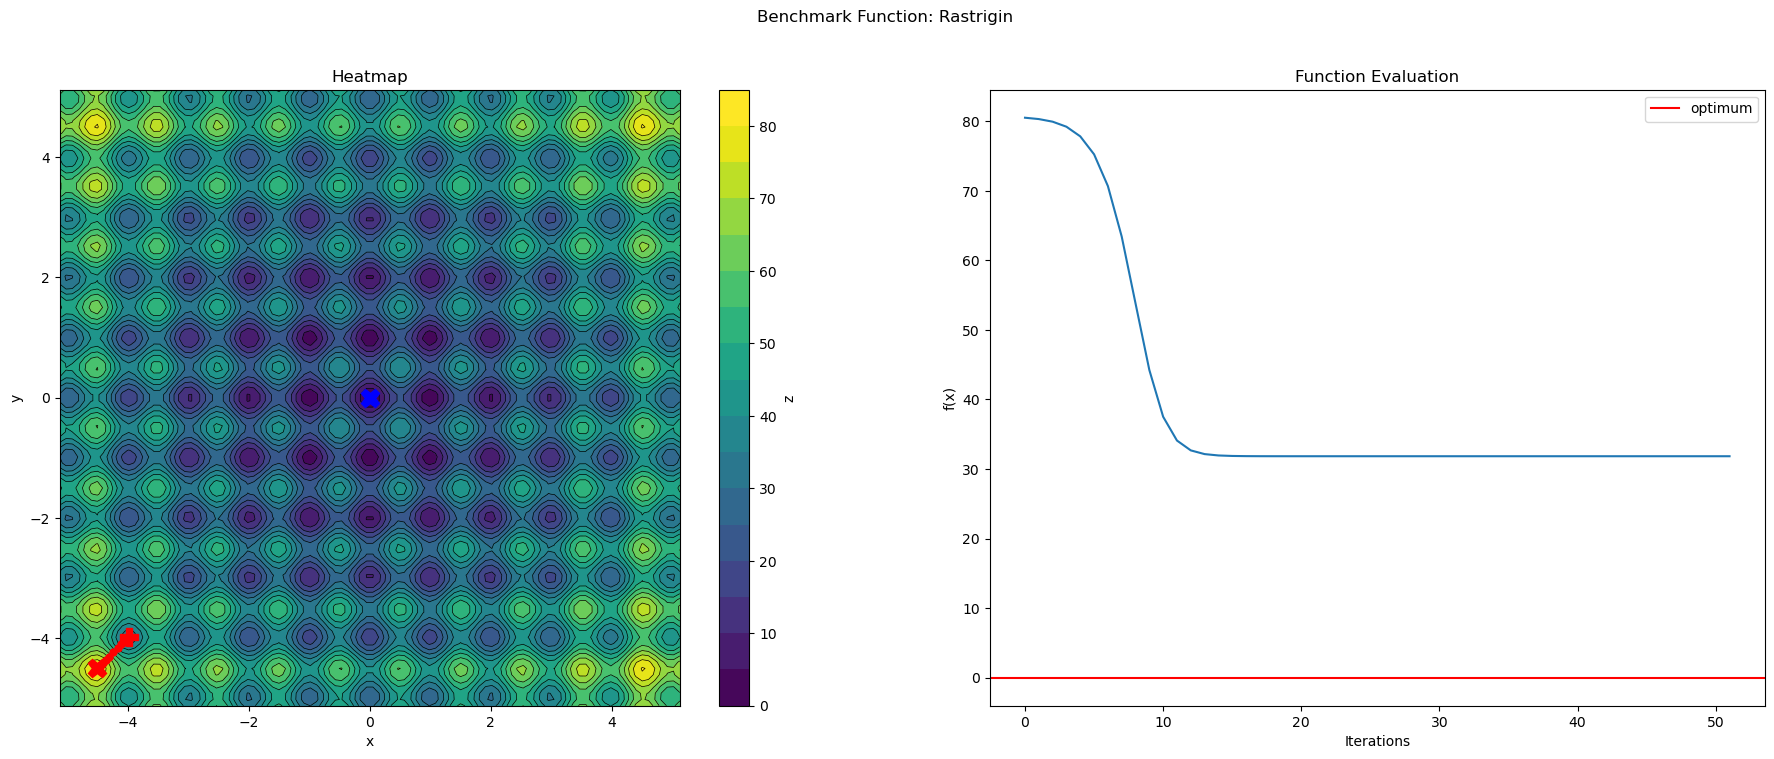
\includegraphics[width=\linewidth]{lab3/imgs/gd_rastr_local.png}
        \caption{Starting point[-4.5,-4.5]}
    \end{subfigure}
    \begin{subfigure}{0.5\linewidth}
        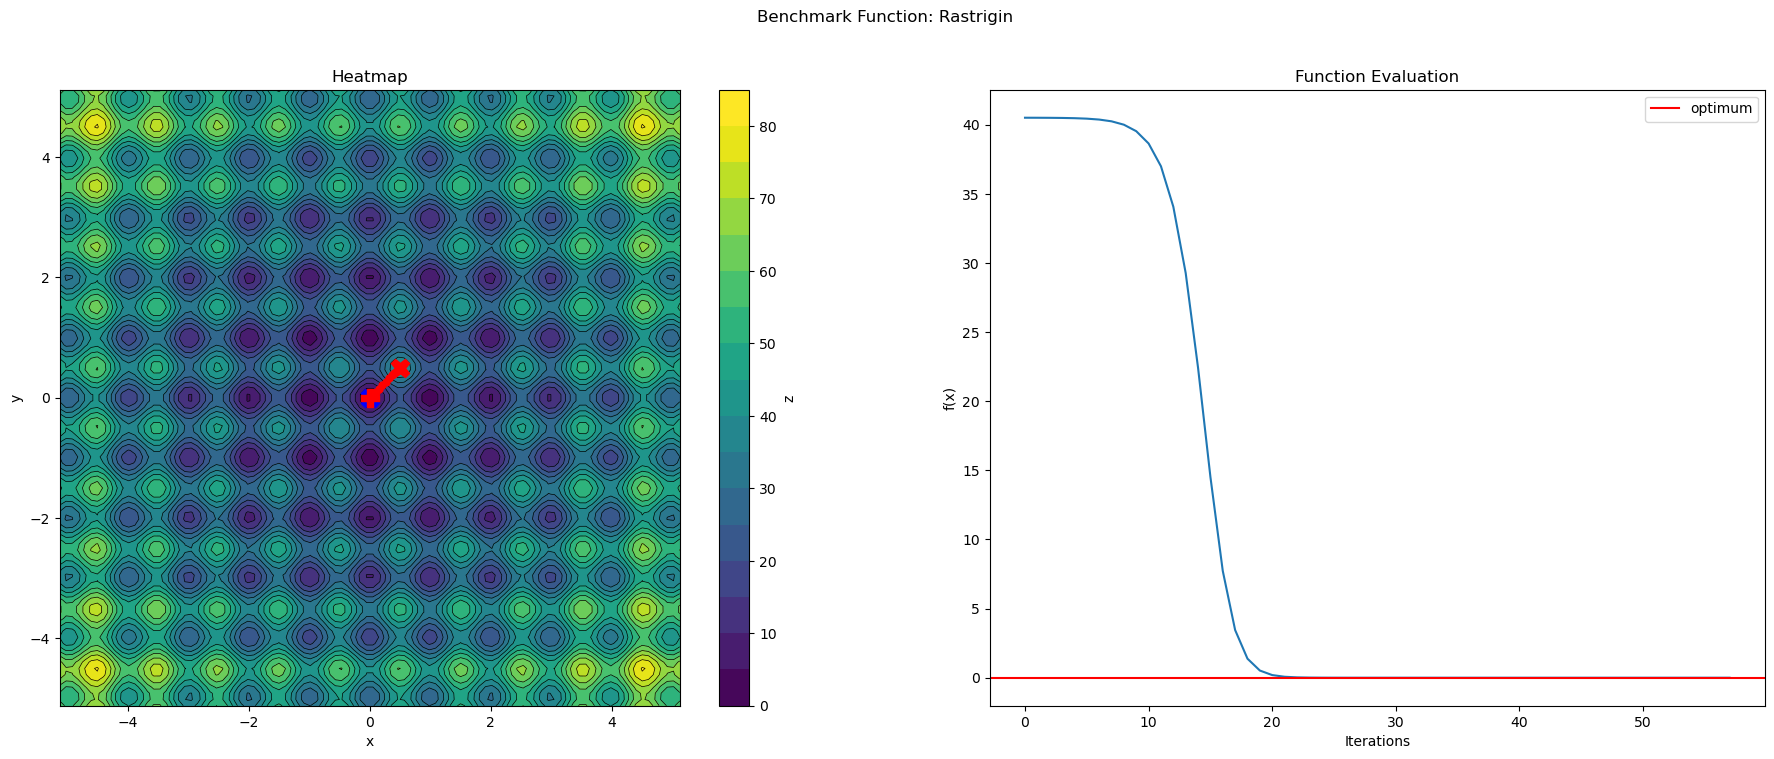
\includegraphics[width=\linewidth]{lab3/imgs/gd_rastr_global.png}
        \caption{Starting point [0.5,0.5]}
    \end{subfigure}
    \caption{Gradient descent on the Rastrigin function}
    \label{fig:gd-rastr}
\end{figure}

It the learning rate is large, gradient descent can also lead to numerical instability and overflow \ref{fig:ros-div}.
\begin{figure}[H]
    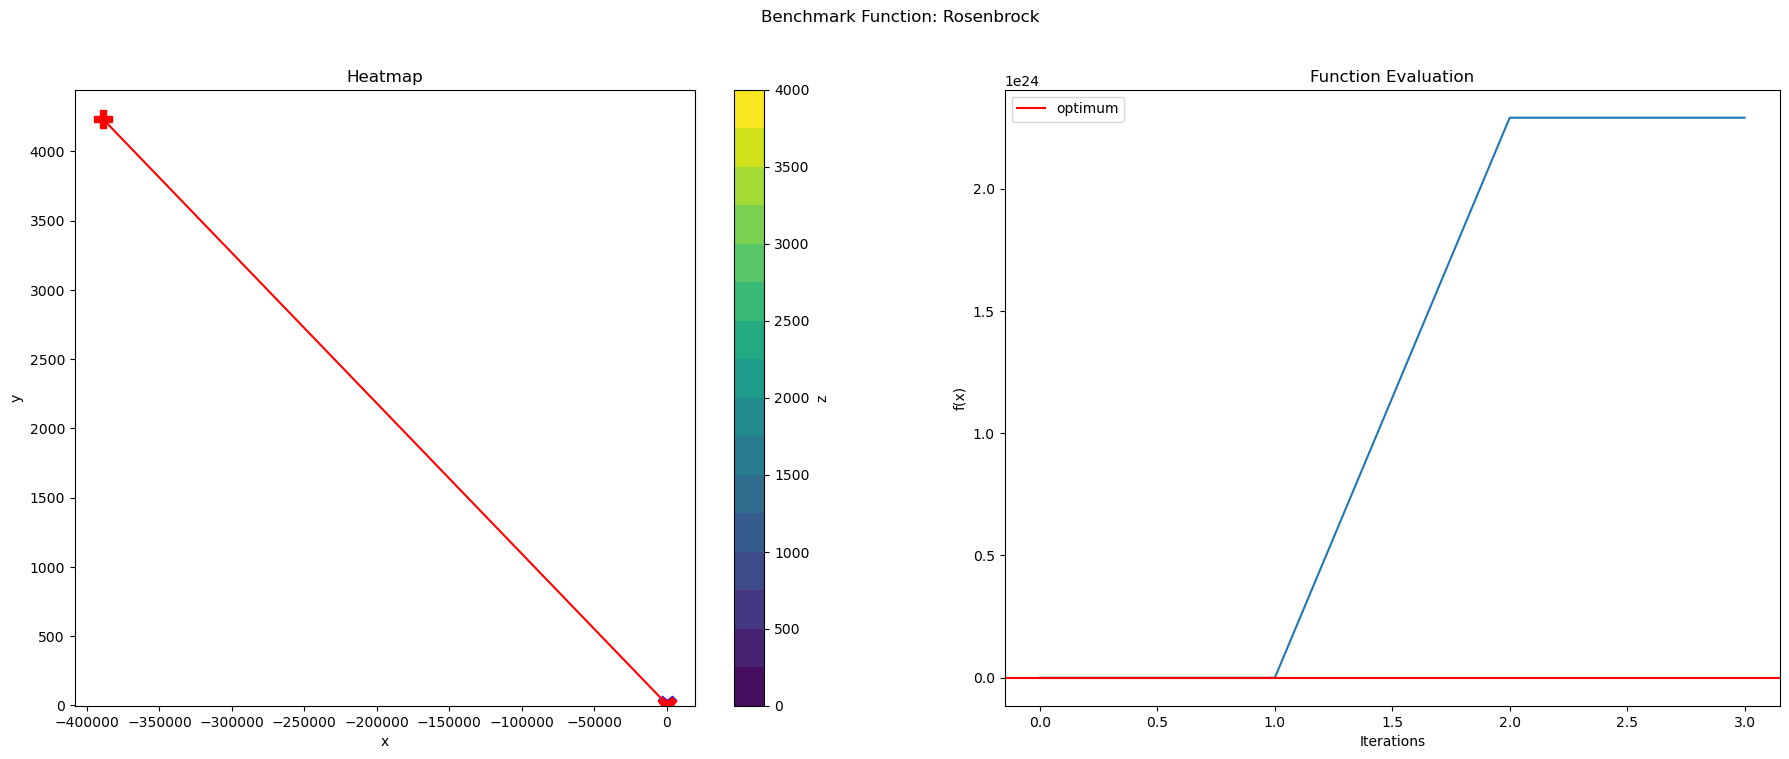
\includegraphics[width=\linewidth]{lab3/imgs/gd_rosenbrock_divergence.png}
    \caption{Gradient descent with learning rate 0.01 on the Rosenbrock function. The algorithm diverges.}
    \label{fig:ros-div}
\end{figure}



\subsection{Newton's Method}
\label{sec:newtons-method}
Newton's method is a second order optimization method, which means that it uses the second derivative of the function to find the minimum. Thus it's more informative than the gradient descent (it doesn't just use the slope of the function, but also the curvature). It can converge faster than gradient descent but it's computationally expensive since it needs to compute the inverse of the Hessian matrix.

Moreover, it has the advantage of having one less parameter to tune (the learning rate) since the algorithm uses instead information about the second derivate of the function to compute the step size.
Even if convergence is on average faster, the same convergence guarantees as the gradient descent apply.

ON the majority of the functions this method doesn't converge or may even founds a worse solution that the original one. Given that this behaviour is not expected, we assume there is a problem in the implementation of the algorithm. We can see this behaviour in the Rastrigin function \ref{fig:nm-rastrigin}.
\begin{figure}[H]
    \centering
    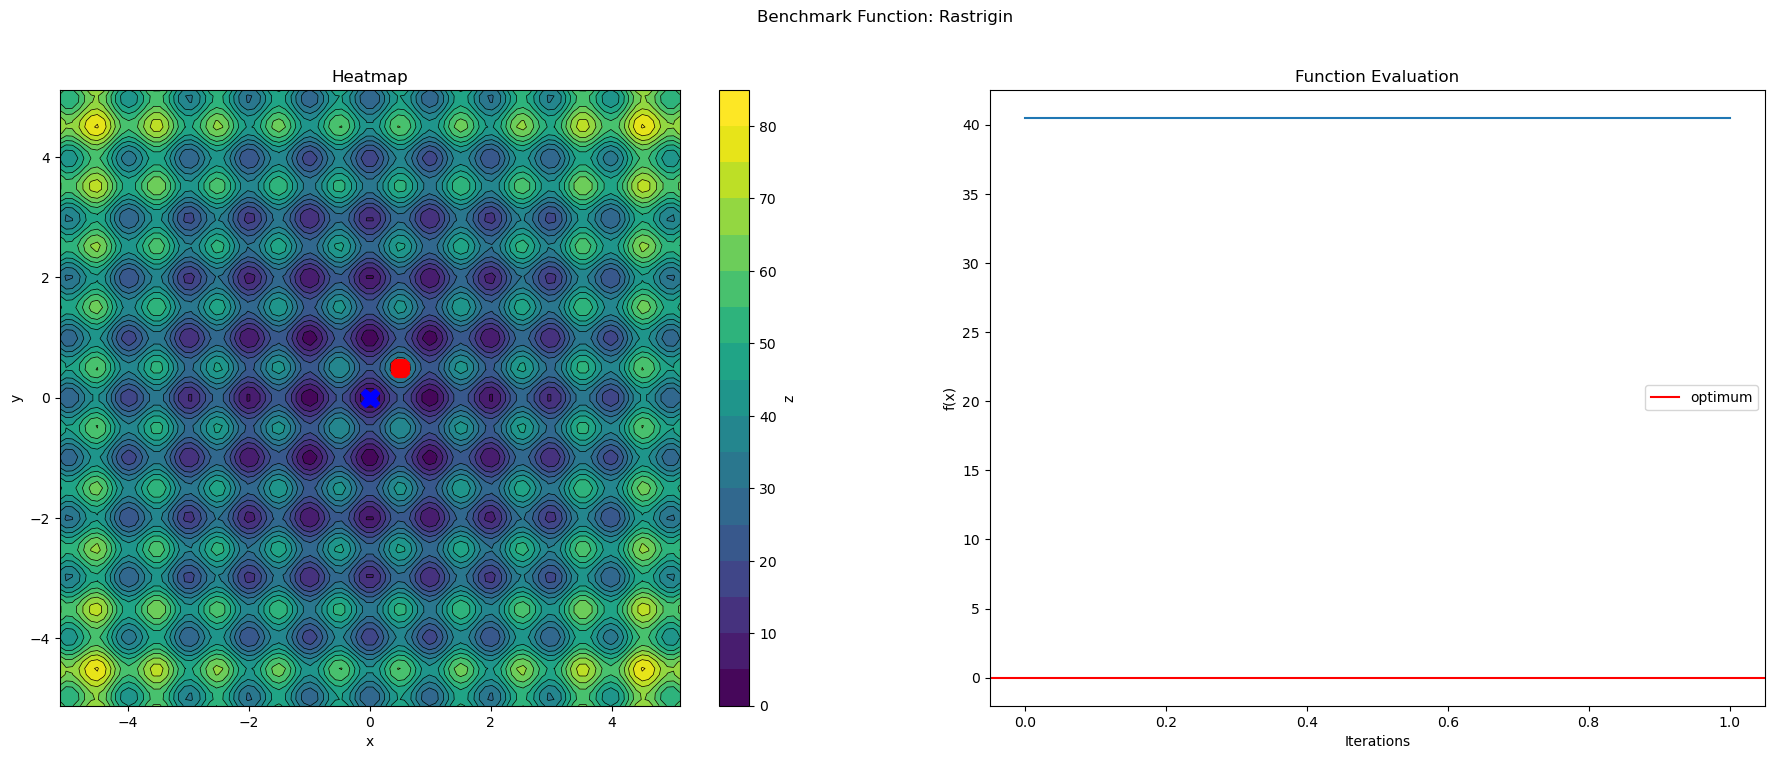
\includegraphics[width=0.8\linewidth]{lab3/imgs/nm_rastrigin.png}
    \caption{Newton's method on the Rastrigin function}
    \label{fig:nm-rastrigin}
\end{figure}


\subsection{BFGS}
\label{sec:bfgs}
BFGS is a quasi-Newton method, which means that it's a second order optimization method that doesn't need to compute the Hessian matrix. It's a good compromise between the gradient descent and Newton's method, since it's faster than the gradient descent but doesn't have the same overhead of computing the Hessian matrix as Newton's methods.

Below \ref{fig:ros-comparison} we report an comparison between the three methods on the Rosenbrock function starting from point [2.0,2.0] and compare the number of iterations needed. It's interesting to notice that the BFGS terminates before reaching the global minimum and even changing the tolerance doesn't help in this case. Nevertheless, we obtain the expected result where the Newton's method converges in the fewest iterations, followed by the BFGS and then gradient descent.
\begin{figure}[H]
    \begin{subfigure}{0.5\linewidth}
        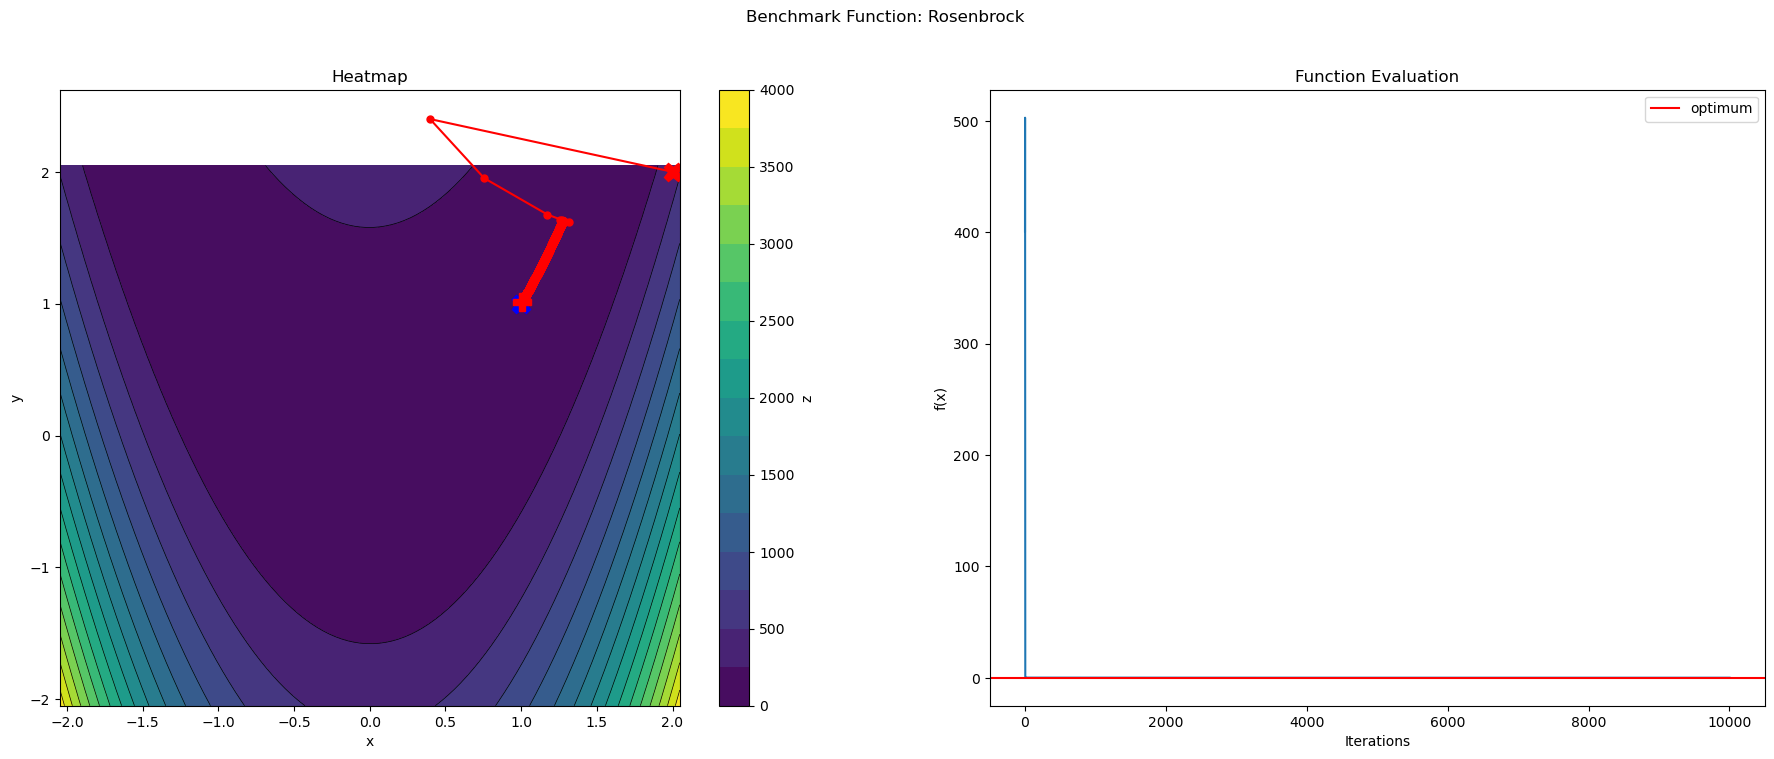
\includegraphics[width=\linewidth]{lab3/imgs/gd_rosenbrock.png}
        \caption{Gradient descent (10000 iterations)}
    \end{subfigure}
    \begin{subfigure}{0.5\linewidth}
        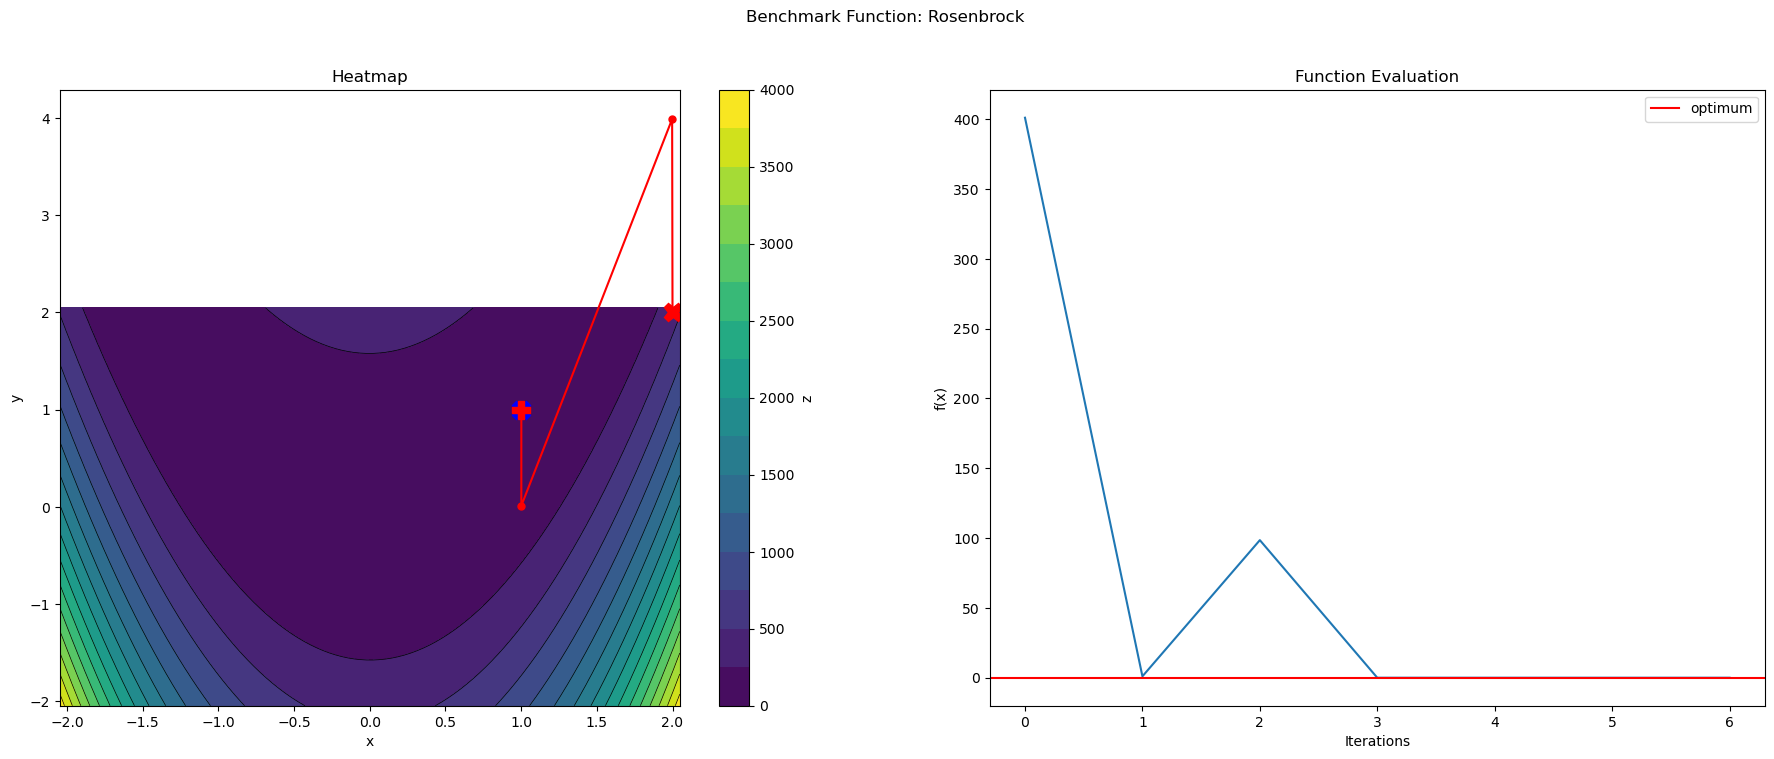
\includegraphics[width=\linewidth]{lab3/imgs/nm_rosenbrock.png}
        \caption{Newton's method (7 iterations)}
    \end{subfigure} \\
    \begin{subfigure}{\linewidth}
        \centering
        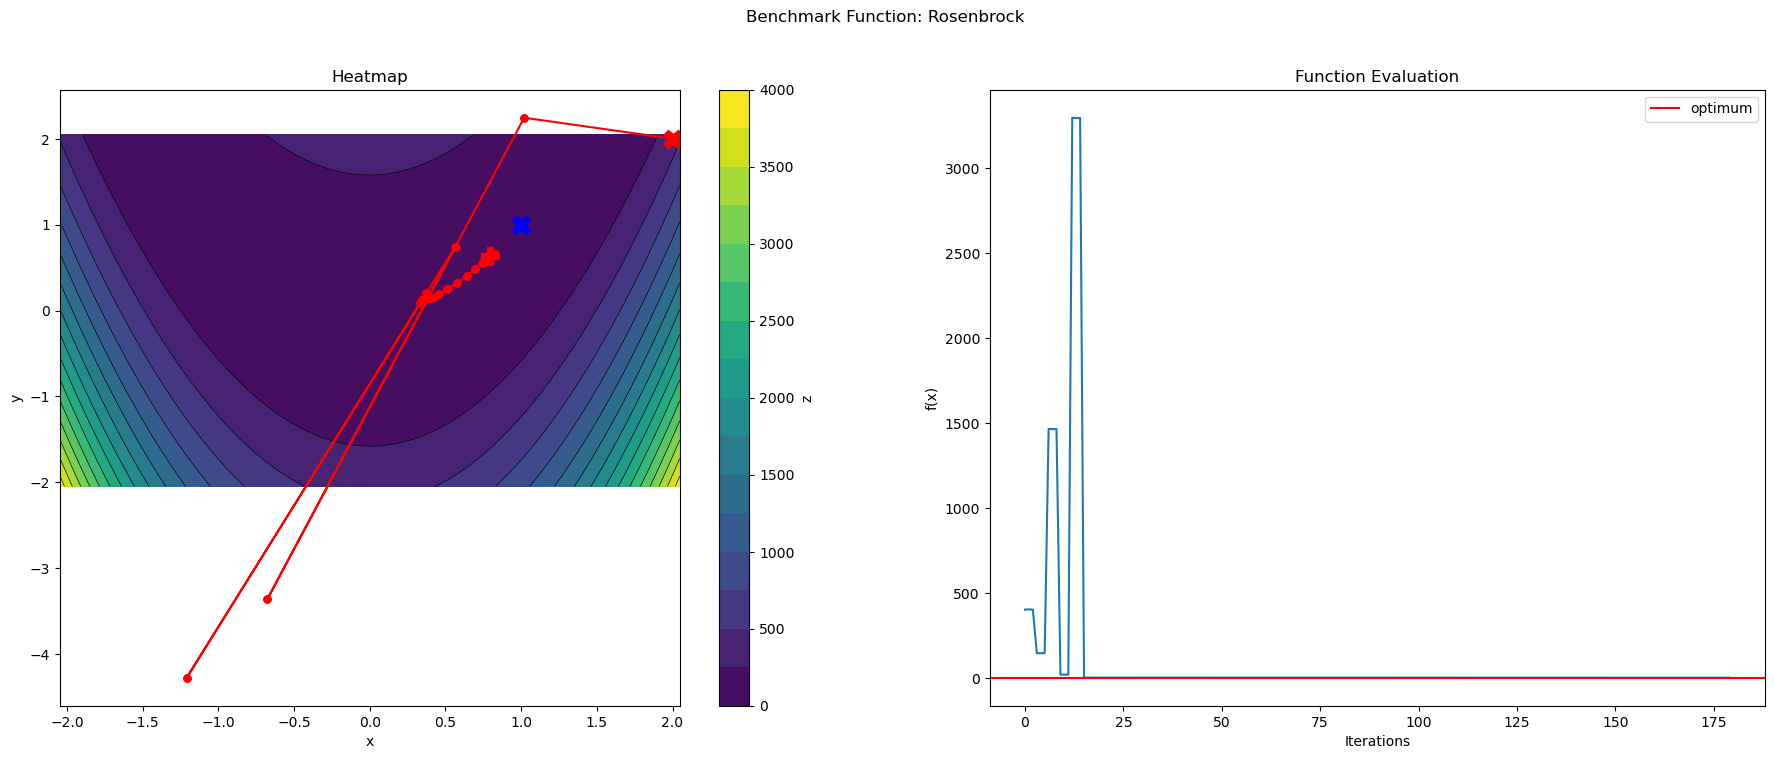
\includegraphics[width=0.5\linewidth]{lab3/imgs/bfgs_rosenbrock.png}
        \caption{BFGS (92 iterations)}
    \end{subfigure}
    \caption{Comparison between Gradient Descent, Newton's Method and BFGS on the Rosenbrock function}
    \label{fig:ros-comparison}
\end{figure}
\newpage

\section{Variable Neighbourhood Search}
\subsection{Variable Neighborhood Search}
Variable Neighborhood Search is a optimization algorithm that combines local search with a neighborhood change strategy. The algorithm is made up of three main components:
\begin{itemize}
    \item Shaking: generates a new solution in the neighborhood of the current solution.
    \item Local Search: improves the solution generated by the shaking step. This is done by applying either first-improvement or best-improvement.
    \item Move or Not: if the solution generated by the local search is better than the current best solution, the current solution is replaced by the new one and the size of the neighborhood is resetted to $k_{min}$. Otherwise, the size of the neighborhood is increased in the hope of finding a better solution in a larger neighborhood.
\end{itemize}

In our example we want to solve the KnapSack-01 problem and  thus the neighborhood structure $N_k$ is defined as the set of all solution that can be obtained by switching $k$ bits in the current solution. Thus it's obvious that the performance of the algorithm is highly dependent on the maximum number of bits that can be switched \ref{tab:neighborhood}. Obviously the quality of the solution achieved is also dependent on the stochastic component of the algorithm.
\begin{table}[H]
    \centering
    \begin{tabular}{c||c |c}
        k  & quantity & capacity \\ \hline
        2  & 8        & 6        \\
        5  & 13       & 8        \\
        7  & 13       & 9        \\
        10 & 15       & 9        \\
    \end{tabular}
    \caption{Different neighborhood structures}
    \label{tab:neighborhood}
\end{table}

On the other hand if we have a diverse enough neighborhood structure, the initial point is not as important as the algorithm will be able to explore the search space anyway \ref{tab:start}.
\begin{table}[H]
    \centering
    \begin{tabular}{c||c |c}
        starting point                 & quantity & capacity \\ \hline
        (1, 0, 0, 1, 0, 1, 0, 1, 0, 1) & 15       & 10       \\
        (0, 1, 0, 1, 1, 1, 0, 1, 0, 0) & 14       & 10       \\
        (1, 1, 1, 1, 1, 1, 1, 1, 1, 1) & 14       & 10       \\
        (0, 0, 0, 0, 0, 0, 0, 0, 0, 0) & 16       & 10       \\
    \end{tabular}
    \caption{Different starting points with $k=10$}
    \label{tab:start}
\end{table}

The other important choice that can be made is the choice of the local search algorithm. Obviously, best-improvement yields better results than first-improvement, but it is also more expensive. In our case, the problem is small enough that there isn't a big difference between the two \ref{fig:vns}.
\begin{figure}[H]
    \begin{subfigure}{0.5\textwidth}
        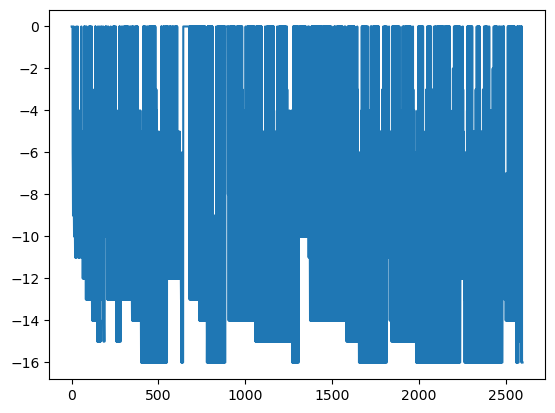
\includegraphics[width=\textwidth]{lab4/imgs/vns_best.png}
        \caption{Best-improvement}
    \end{subfigure}
    \begin{subfigure}{0.5\textwidth}
        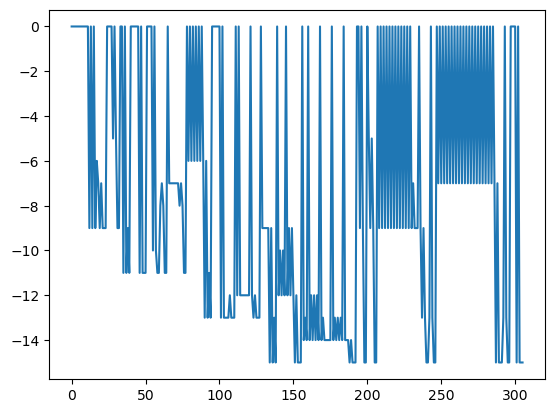
\includegraphics[width=\textwidth]{lab4/imgs/vns_first.png}
        \caption{First-improvement}
    \end{subfigure}
    \caption{VNS with different local search algorithms}
    \label{fig:vns}
\end{figure}


\subsection{Reduced Variable Neighborhood Search}
Reduced Variable Neighborhood Search is a variant of the VNS algorithm that skips the most expensive step of VNS which is the local search.

Similarly to VNS, if the neighborhood structure is diverse enough the starting is not very important \ref{tab:rvns-start} but if the neighborhood is limited then it becomes very important. For example in table \ref{tab:rvns-neigh} we can see that for $k=2$ the algorithm was unable to find a valid solution.
\begin{table}[H]
    \centering
    \begin{tabular}{c||c |c}
        starting point                 & quantity & capacity \\ \hline
        (1, 0, 0, 1, 0, 1, 0, 1, 0, 1) & 13       & 8        \\
        (0, 1, 0, 1, 1, 1, 0, 1, 0, 0) & 15       & 10       \\
        (1, 1, 1, 1, 1, 1, 1, 1, 1, 1) & 12       & 10       \\
        (0, 0, 0, 0, 0, 0, 0, 0, 0, 0) & 11       & 9        \\
    \end{tabular}
    \caption{Different starting points}
    \label{tab:rvns-start}
\end{table}
\begin{table}[H]
    \centering
    \begin{tabular}{c||c |c}
        k  & quantity & capacity \\ \hline
        2  & 0        & 0        \\
        5  & 11       & 10       \\
        7  & 14       & 10       \\
        10 & 13       & 10       \\
    \end{tabular}
    \caption{Different neighborhood structures}
    \label{tab:rvns-neigh}
\end{table}
\newpage

\section{Iterated Local Search, Simulated Annealing}
In this lab, we will implement two different optimization methods for the Knapsack problem: Iterated Local Search and Simulated Annealing.
\subsection{Iterated Local Search}
Iterated Local Search (ILS) is a stochastic local search method that generates a sequence of solutions generated by an embedded heuristic. It can be seen as a family of algorithms based on the same basic procedure:
\begin{enumerate}
    \item Generate an initial solution $s$.
    \item Repeat until a stopping criterion is met:
          \begin{enumerate}
              \item Apply a local search procedure to $s$ to obtain a local minimum $s'$.
              \item Perturb $s'$ to obtain a new solution $s$.
              \item Accept $s$ as the new current solution based on some acceptance criterion.
          \end{enumerate}
\end{enumerate}
ILS can be seen as a general framework that can be instantiated in many ways bu choosing different local search procedures, perturbation mechanisms and intensities, and acceptance criteria. In this instance, we are basically reimplementing the Variable Neighborhood Search (VNS) algorithm (see lab 4 for more details).


\subsection{Simulated Annealing}
Simulated Annealing is a optimization algorithm inspired by the annealing process in metallurgy. The algorithm starts with an initial solution and iteratively moves to a new solution. The new solution is accepted if it improves upon the current solution or with a probability that decreases with time. The probability of accepting a solution that is worse than the current solution is given by the Metropolis criterion $p = e^{-(f(x')-f(x))/T}$. The temperature $T$ is a parameter that controls the probability of accepting a worse solution and is decreased over time according to a cooling schedule ($T = \alpha T$).

The first parameter that we need to evaluate is the temperature $T$ \ref{tab:sa-temp}. As we can see, the best performance is achieved with $T=1$ or smaller which makes sense since the difference in the objective function is small.
\begin{table}[H]
    \centering
    \begin{tabular}{c||c |c}
        T    & quantity & capacity \\ \hline
        0.1  & 14.62    & 9.79     \\
        0.5  & 14.64    & 9.88     \\
        1.0  & 14.65    & 9.83     \\
        5.0  & 13.72    & 9.61     \\
        10.0 & 12.94    & 9.22     \\
    \end{tabular}
    \caption{Different temperatures}
    \label{tab:sa-temp}
\end{table}

The initial solution doesn't seem to be important for the performance of the algorithm \ref{tab:sa-start}
\begin{table}[H]
    \centering
    \begin{tabular}{c||c |c}
        starting point                 & quantity & capacity \\ \hline
        (1, 0, 0, 1, 0, 1, 0, 1, 0, 1) & 14.72    & 9.82     \\
        (0, 1, 0, 1, 1, 1, 0, 1, 0, 0) & 14.61    & 9.85     \\
        (1, 1, 1, 1, 1, 1, 1, 1, 1, 1) & 14.79    & 9.84     \\
        (0, 0, 0, 0, 0, 0, 0, 0, 0, 0) & 14.63    & 9.8      \\
    \end{tabular}
    \caption{Different starting points with $k=10$ and $T=1$}
    \label{tab:sa-start}
\end{table}

Differently from ILS and VNS, the nieghbourhood structure is not as important for the performance of the algorithm \ref{tab:sa-neigh} probably due to the different accepting criteria used that allows the algorithm to explore the search space more freely. Even though the difference is small, the best performance is still achieved with $k=10$.
\begin{table}[H]
    \centering
    \begin{tabular}{c||c |c}
        k  & quantity & capacity \\ \hline
        2  & 11.85    & 9.5      \\
        5  & 14.49    & 9.81     \\
        7  & 14.63    & 9.83     \\
        10 & 14.7     & 9.79     \\
    \end{tabular}
    \caption{Different neighborhood structures and $T=1$}
    \label{tab:sa-neigh}
\end{table}

The last parameter that we need to evaluate is the cooling schedule. We can see that the performance of the algorithm is not very sensitive to the choice of the cooling schedule \ref{tab:sa-cool}.
\begin{table}[H]
    \centering
    \begin{tabular}{c||c |c}
        k   & quantity & capacity \\ \hline
        0.1 & 14.58    & 9.74     \\
        0.3 & 14.65    & 9.80     \\
        0.5 & 14.70    & 9.81     \\
        0.7 & 14.70    & 9.79     \\
        0.9 & 14.45    & 9.74     \\
    \end{tabular}
    \caption{Different cooling schedules and $T=1$ and $k=10$}
    \label{tab:sa-cool}
\end{table}
\newpage

\section{Bayesian Optimization}
Bayesian Optimization is a optimization algorithm that uses a probabilistic model to approximate the objective function \textit{(surrogate model)} and uses this model to guide the search for the optimal solution. The general procedure can be described as follows:
\begin{enumerate}
    \item choose surrogate function that approximates the real objective function (prior)
    \item repeat until stopping condition
          \begin{enumerate}
              \item given a number of observations (computed from the real objective function), update the surrogate function (posterior distribution). Default choice is usually a Gaussian Process
              \item optimize a cheap \textit{acquisition function / utility function} based on the posterior distribution to find the new point to sample. Also has the responsability of balancing exploration and exploitation
          \end{enumerate}
\end{enumerate}

\paragraph*{Choice of Prior}
In this lab, we'll use three different prior distribution to sample the initial points for the optimization algorithm. The three distributions are:
\begin{itemize}
    \item \textit{Prior1}: Uniform in the range $[0, 1]$
    \item \textit{Prior2}: Uniform in the range $[0, 0.5]$
    \item \textit{Prior3}: Uniform in the range $[0.5, 1]$
\end{itemize}
\begin{table}[H]
    \centering
    \begin{tabular}{|c|c|c|}
        \textbf{Prior} & \textbf{Mean}    & \textbf{Std. Deviation} \\\hline
        Prior1         & (0.9967, 1.0966) & (0.0026, 0.0198)        \\
        Prior2         & (0.9963, 1.0999) & (0.0043, 0.0206)        \\
        Prior3         & (0.6991, 0.7897) & (0.4528, 0.4687)        \\
        \hline
    \end{tabular}
    \caption{Best point found with Objective1 and UCB acquisition function}
    \label{tab:prior}
\end{table}
We can see that Prior3 achieves worse results due to the fact that the prior distribution doesn't cover the optimal region. In particular the standard deviation is very high, which means tha the Bayesian Optimzation found good solutions in some cases but it's not consistent.

\begin{figure}[H]
    \begin{subfigure}{0.5\textwidth}
        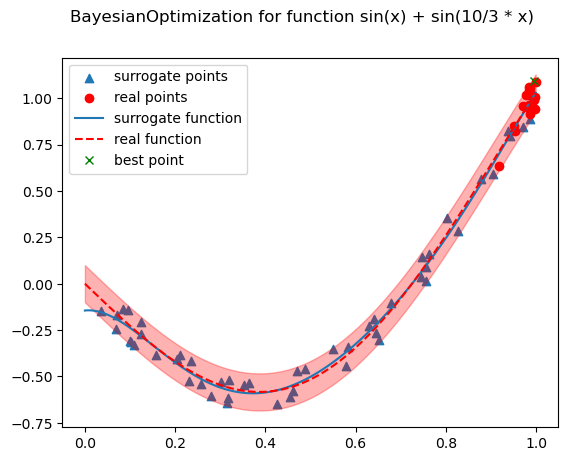
\includegraphics[width=\textwidth]{lab6/imgs/obj1_pr1.png}
        \caption{Prior1}
    \end{subfigure}
    \begin{subfigure}{0.5\textwidth}
        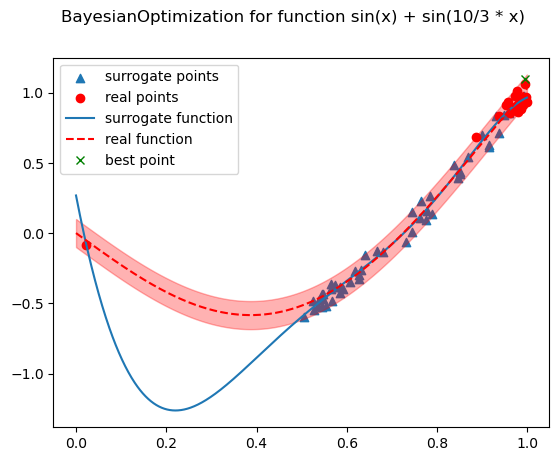
\includegraphics[width=\textwidth]{lab6/imgs/obj1_pr2.png}
        \caption{Prior2}
    \end{subfigure} \\
    \begin{subfigure}{\textwidth}
        \centering
        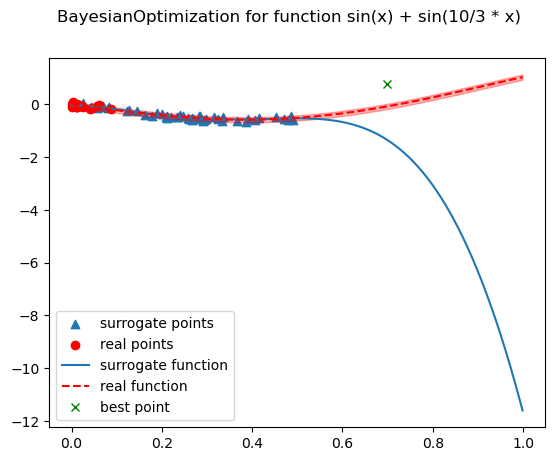
\includegraphics[width=0.5\textwidth]{lab6/imgs/obj1_pr3.png}
        \caption{Prior3}
    \end{subfigure}
    \caption{Objective1 with different prior distribution}
    \label{fig:bo-prior}
\end{figure}
It's also interesting to note how the Gaussian Process differently approximate the real objective function based on the prior distribution: Prior1 better approximates the real function since it covers the entire range of the function.

\paragraph*{Acquisition Function}
The results are roughly the same for all the acquisition functions, with EI slightly worse than the others.
\begin{table}[H]
    \centering
    \begin{tabular}{|c|c|c|}
        \textbf{Prior} & \textbf{Mean}    & \textbf{Std. Deviation} \\\hline
        UCB            & (0.9715, 1.5490) & (0.0055, 0.0202)        \\
        LCB            & (0.9688, 1.5527) & (0.0070, 0.0297)        \\
        PI             & (0.9661, 1.5107) & (0.0101, 0.0556)        \\
        EI             & (0.9693, 1.4752) & (0.0142, 0.0649)        \\
        \hline
    \end{tabular}
    \caption{Best point found with Objective1 and UCB acquisition function}
    \label{tab:acquisition}
\end{table}

\begin{figure}[H]
    \begin{subfigure}{0.5\textwidth}
        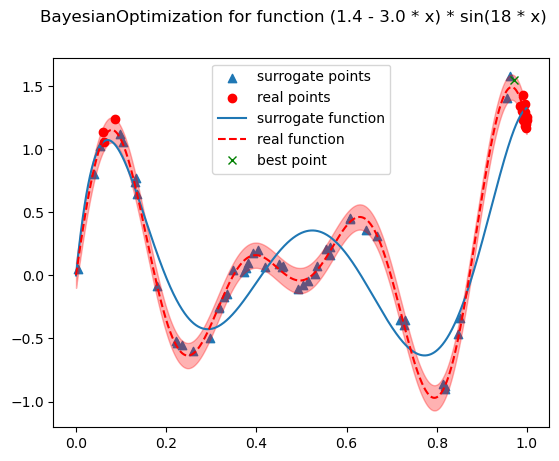
\includegraphics[width=\textwidth]{lab6/imgs/obj2_ucb.png}
        \caption{UCB}
    \end{subfigure}
    \begin{subfigure}{0.5\textwidth}
        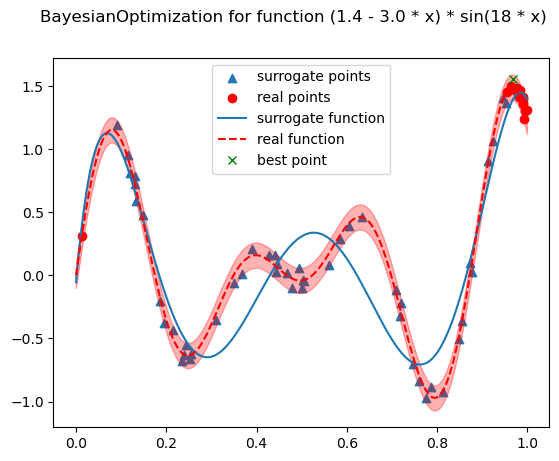
\includegraphics[width=\textwidth]{lab6/imgs/obj2_lcb.png}
        \caption{LCB}
    \end{subfigure} \\
    \begin{subfigure}{0.5\textwidth}
        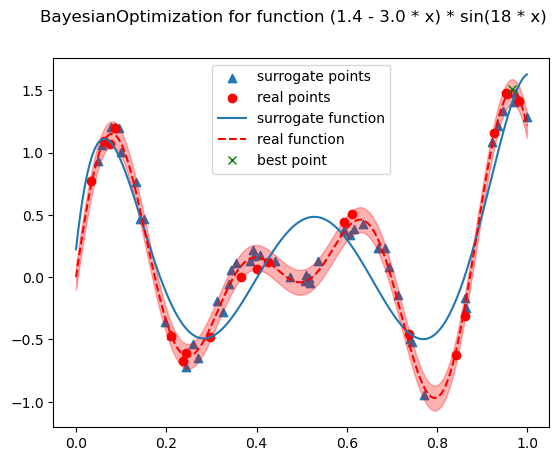
\includegraphics[width=\textwidth]{lab6/imgs/obj2_pi.png}
        \caption{PI}
    \end{subfigure}
    \begin{subfigure}{0.5\textwidth}
        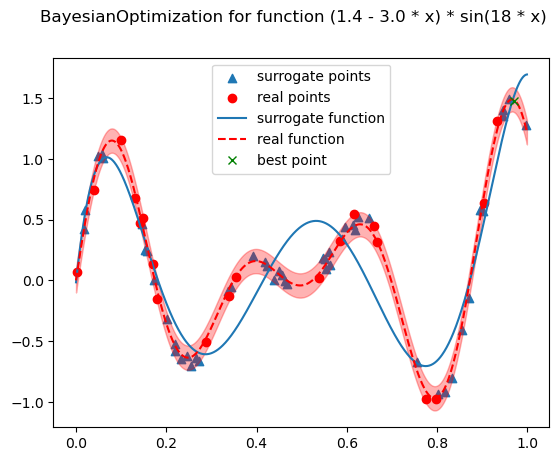
\includegraphics[width=\textwidth]{lab6/imgs/obj2_ei.png}
        \caption{EI}
    \end{subfigure}
    \caption{Objective2 with different acquisition functions}
    \label{fig:bo-acquisition}
\end{figure}
We can see that the acquisition functions have two main behavious: UCB and LCB focus right away on the optimal region while PI and EI are more focused on the exploration of the space.

\paragraph*{Kernel}
\begin{table}[H]
    \centering
    \begin{tabular}{|c|c|c|}
        \textbf{Kernel} & \textbf{Mean}  & \textbf{Std. Deviation} \\\hline
        RBF             & (0.8909, 1.7960) & (0.0500, 0.1031)          \\
        DotProduct      & (0.8937, 1.7634) & (0.0399, 0.1153)          \\
        ExpSineSquared  & (0.8828, 1.7768) & (0.0599, 0.1307)          \\
        \hline
    \end{tabular}
    \caption{Best point found with Objective3 and UCB acquisition function}
    \label{tab:kernel}
\end{table}
The results are roughly the same for all the kernels and all have quite high variance.

\begin{figure}[H]
    \begin{subfigure}{0.5\textwidth}
        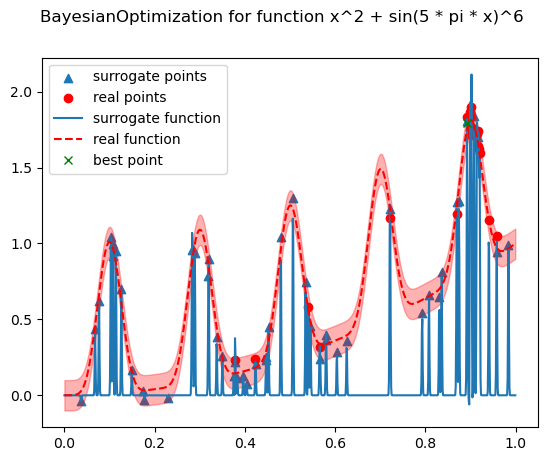
\includegraphics[width=\textwidth]{lab6/imgs/obj3_rbf.png}
        \caption{RBF}
    \end{subfigure}
    \begin{subfigure}{0.5\textwidth}
        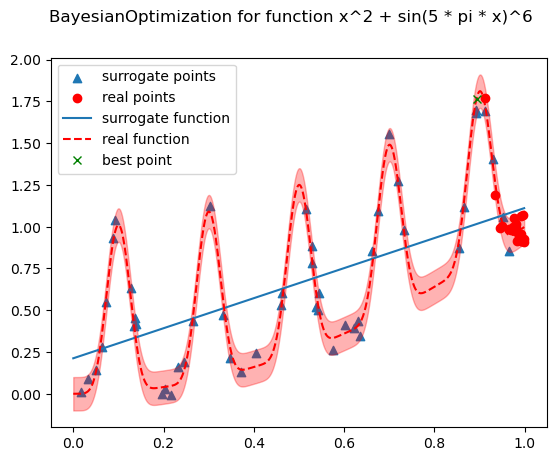
\includegraphics[width=\textwidth]{lab6/imgs/obj3_dot.png}
        \caption{DotProduct}
    \end{subfigure} \\
    \begin{subfigure}{\textwidth}
        \centering
        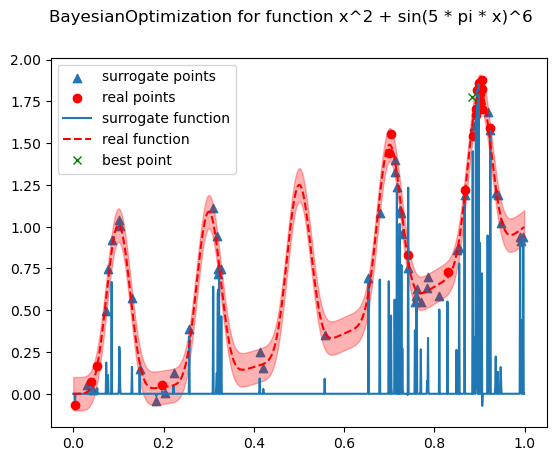
\includegraphics[width=0.5\textwidth]{lab6/imgs/obj3_exp.png}
        \caption{ExpSineSquared}
    \end{subfigure}
    \caption{Objective3 with different kernels}
    \label{fig:bo-kernel}
\end{figure}
We can see that differently than without the kernel, the Gaussian Process in not able to approximate the real function well but the sampled points are still in the optimal region. Moreover, in some cases the Gaussian Process with the kernel isn't able to converge, possibly due to kernel's hyperparameters that are not well tuned.

\newpage

\section{Genetic, Evolution and Nature-Inspired Analogies}
\subsection{Genetic Algorithms}
Genetic algortithms are a class of metaheiristics ispired by the process of natural selection where the best individuals are the ones with the best fitness/objective function value. The general schema of GA is as follows:
\begin{enumerate}
    \item Generate an initial population of individuals.
    \item Evaluate the fitness of each individual.
    \item Repeat until the termination condition is met:
          \begin{enumerate}
              \item Select individuals for reproduction.
              \item Crossover and mutate the selected individuals.
              \item Evaluate the fitness of the new individuals.
              \item Replace the old population with the new population.
          \end{enumerate}
\end{enumerate}

Except if differently specified, the following parameters are used for all following experiments:
\begin{itemize}
    \item Population size: 50
    \item Number of generations: 50
    \item Objective function: Ackley
    \item Gaussia mutation with stadard deviation 1.0
    \item Number of simulations: 10
\end{itemize}

\paragraph*{Mutation only GA}
The GA with only mutation has slightly worse performance for high mutation rates probably because the perturbation is too big to precisely converge to the optimum but in general it achieves satisfactory performances. The results are shown in Table \ref{tab:mutation_rate}.
\begin{table}[H]
    \centering
    \begin{tabular}{|c|c|c|}
        Mutation rate & Average fitness & Standard deviation \\ \hline
        0.1           & 0.0435          & 0.0244             \\
        0.2           & 0.0355          & 0.0183             \\
        0.3           & 0.0425          & 0.0297             \\
        0.4           & 0.0568          & 0.0233             \\
        0.5           & 0.0621          & 0.0177             \\
        0.6           & 0.1061          & 0.0585             \\
        0.7           & 0.0733          & 0.0601             \\
        0.8           & 0.1021          & 0.0596             \\
        0.9           & 0.1222          & 0.0819             \\
        1.0           & 0.1787          & 0.0863             \\
    \end{tabular}
    \caption{Mutation rate only}
    \label{tab:mutation_rate}
\end{table}

\paragraph*{Crossover only GA}
We now test the case where only crossover is used and we notice how the algorithm is not able to find a good solution. This is beacuse without mutation there is no introduction of new genetic material so the algorithm is not able to explore the search space. The results are shown in Table \ref{tab:crossover_rate}.
\begin{table}[H]
    \centering
    \begin{tabular}{|c|c|c|}
        Crossover rate & Average fitness & Standard deviation \\ \hline
        0.1            & 7.997           & 0.0863             \\
        0.2            & 8.234           & 0.0863             \\
        0.3            & 7.376           & 0.0863             \\
        0.4            & 5.875           & 0.0863             \\
        0.5            & 5.798           & 0.0863             \\
        0.6            & 5.224           & 0.0863             \\
        0.7            & 4.660           & 0.0863             \\
        0.8            & 5.539           & 0.0863             \\
        0.9            & 6.538           & 0.0863             \\
        1.0            & 6.366           & 0.0863             \\
    \end{tabular}
    \caption{Crossover rate only}
    \label{tab:crossover_rate}
\end{table}

\paragraph*{Tournament size}
We now test the tournament size selection method. We can see that the best performances are obtained for large tournament sizes. This is because the selection pressure is higher and the Ackely function has many local minima but none of them are "deceptive" so the algorithm can forego exploration and focus on exploitation. The results are shown in Table \ref{tab:tournament_size}.
\begin{table}[H]
    \centering
    \begin{tabular}{|c|c|c|}
        Tournament size & Average fitness & Standard deviation \\ \hline
        1               & 0.8596          & 0.9068             \\
        5               & 0.0233          & 0.0157             \\
        10              & 0.0435          & 0.0138             \\
        20              & 0.0238          & 0.0135             \\
        30              & 0.0206          & 0.0164             \\
        40              & 0.0124          & 0.0084             \\
        50              & 0.0188          & 0.0188             \\
    \end{tabular}
    \caption{Diferent tournament sizes with mutation rate 0.2 and crossover rate 0.7}
    \label{tab:tournament_size}
\end{table}

\paragraph*{Compare different objective functions}
All the results are shown in Figure \ref{fig:ga-comp} with mutation rate 0.2, crossover rate 0.7. The results are comparable for all functions taking into account that different functions have different characteristics and the used parameters are not optimized for each function.
\begin{figure}[H]
    \begin{subfigure}{0.5\textwidth}
        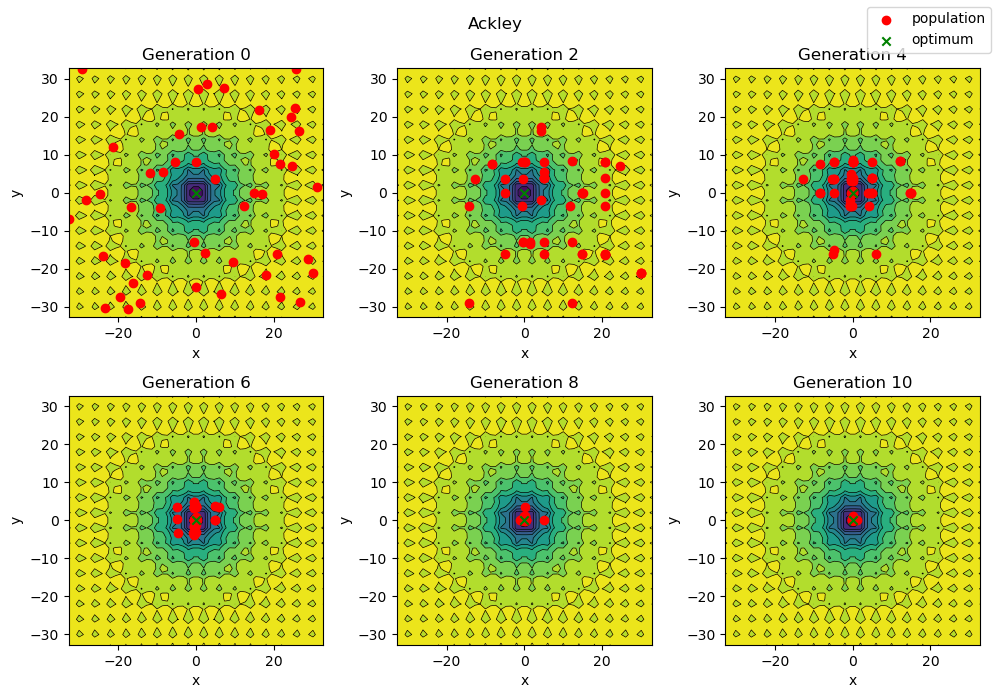
\includegraphics[width=\textwidth]{lab7/imgs/ga_ackley.png}
        \caption{Ackley function}
    \end{subfigure}
    \begin{subfigure}{0.5\textwidth}
        \includegraphics[width=\textwidth]{lab7/imgs/ga_rastrigin.png}
        \caption{Rastringin function}
    \end{subfigure}\\
    \begin{subfigure}{0.5\textwidth}
        \includegraphics[width=\textwidth]{lab7/imgs/ga_hypersphere.png}
        \caption{Hypersphere function}
    \end{subfigure}
    \begin{subfigure}{0.5\textwidth}
        \includegraphics[width=\textwidth]{lab7/imgs/ga_rosenbrock.png}
        \caption{Rosenbrock function}
    \end{subfigure}
    \caption{Comparison of different objective functions for the GA algorithm}
    \label{fig:ga-comp}
\end{figure}



\subsection{Evolution Strategies}
Evolution Strategies are a class of metaheuristics that are similar to genetic algorithms but only use mutation and evolve the mutation operator together with the individual.

Unless specified, the following parameters are used:
\begin{itemize}
    \item Population size: 50
    \item Number of generations: 50
    \item Objective function: Ackley
    \item Strategy: None
    \item Number of simulations: 10
\end{itemize}

\paragraph*{Offspring size}
We can see that the performance of the algorithm is better for larger offspring sizes. This is because the algorithm is able to explore the search space better but with the tradeoff of computational complexity. The results are shown in Table \ref{tab:es-offspring_size}.
\begin{table}[H]
    \centering
    \begin{tabular}{|c|c|c|}
        Offspring size & Average fitness & Standard deviation \\ \hline
        50             & 0.0920          & 0.0699             \\
        100            & 0.0787          & 0.0303             \\
        200            & 0.0325          & 0.0238             \\
        300            & 0.0236          & 0.0099             \\
        400            & 0.0104          & 0.0108             \\
        500            & 0.0282          & 0.0131             \\
    \end{tabular}
    \caption{Different offspring sizes with mutation rate 0.2}
    \label{tab:es-offspring_size}
\end{table}

\paragraph*{Strategy}
We now test different strategy to evolve the mutation rate:
\begin{itemize}
    \item None: the mutation rate is fixed
    \item Global: each individual evolves a single mutation rate (sphere)
    \item Individual: each individual has a mutation rate for each gene / dimension (axis-parallel ellipsoid)
    \item Correlated: each individual has a mutation rate for each gene and the interaction between every pair of genes (general ellipsoid)
\end{itemize}
We can see that the best performance is obtained with the global strategy probably because there is no skewed narrow vallet to be found in the Ackely function that would require a more complex strategy. The results are shown in Table \ref{tab:es-strategy}.
\begin{table}[H]
    \centering
    \begin{tabular}{|c|c|c|}
        Strategy   & Average fitness & Standard deviation \\ \hline
        None       & 4.57e-02        & 1.91e-02           \\
        Global     & 1.41e-06        & 4.09e-07           \\
        Individual & 1.75e-04        & 2.51e-04           \\
        Correlated & 6.38e-02        & 1.10e-01           \\
    \end{tabular}
    \caption{Different strategies with offspring size 100}
    \label{tab:es-strategy}
\end{table}

\subsection{Particle Swarm Optimization}
Particle Swarm Optimization is a population-based optimization technique that is inspired by the social behavior of flocks of birds searching for food. The algorithms aims at finding emerging social behaviours starting from few simple local rules. These rules are:
\begin{itemize}
    \item each position in the environment is associated with a reward
    \item each particle has memory of the best position it visited
    \item each particle gets information from its neighbours
\end{itemize}

\paragraph*{Population size / Generation ratio}
We compare the performances of the algorithm by changing the number of individuals in the population and the number of generations but keeping the ratio constant (so to have the same number of evaluations). We can see that the performance is better for larger populations and smaller number of generations. The results are shown in Table \ref{tab:pso-pop-gen}.
\begin{table}[H]
    \centering
    \begin{tabular}{|c|c|c|c|}
        Population size & Generations & Average fitness & Standard deviation \\ \hline
        20              & 125         & 7.99e-16        & 1.74e-15           \\
        40              & 62          & 1.02e-11        & 5.92e.12           \\
        60              & 41          & 7.53e-08        & 3.05e-08           \\
        80              & 31          & 4.30e-06        & 1.99e-06           \\
        100             & 25          & 4.05e-05        & 4.05e-05           \\
    \end{tabular}
    \caption{Different population sizes and generation numbers with mutation rate 0.2}
    \label{tab:pso-pop-gen}
\end{table}

\paragraph*{Topology}
We now test different topologies for the algorithm:
\begin{itemize}
    \item Ring: each particle gets information from the N closest particles
    \item Star: each particle gets information from all other particles
\end{itemize}
The best performances are obtained by the star topology because the each particle gets information by a larger number of particles. To confirm this trend, we can see that the performance of the ring topology increases with the number of neighbours. The results are shown in Table \ref{tab:pso-topology}.
\begin{table}[H]
    \centering
    \begin{tabular}{|c|c|c|}
        Topology & Average fitness & Standard deviation \\ \hline
        Star     & 1.62e-09        & 1.16e-09           \\
        Ring 2   & 4.58e-04        & 3.67e-04           \\
        Ring 5   & 2.37e-07        & 3.24e-07           \\
        Ring 10  & 1-90e-08        & 2.31e-08           \\
        Ring 20  & 4.22e-09        & 2.24e-09           \\
        Ring 30  & 3.18e-09        & 1.97e-09           \\
        Ring 40  & 2.80e-09        & 1.71e-09           \\
    \end{tabular}
    \caption{Different topologies with population size 40 and generation number 62}
    \label{tab:pso-topology}
\end{table}
\newpage

\section{Multi-Objective Optimization}
Multi-objective optimization is characterized by the presence of multiple, possibly conflicting, objectives. This means that the optimal solution for any single objective doesn't necessarily correspond to the optimal solution for the other objectives. What we get instead is a set of solutions that are optimal in the sense that no other solution is better in all objectives. This set of solutions is called the Pareto front.

The state of the art in multi-objective optimization is the NSGA-II algorithm, which is a genetic algorithm that uses a non-dominated sorting approach to create fronts of solutions that are not dominated by any other solution. The algorithm then selects the best solutions from the fronts, ensuring that the population is diverse and that the Pareto front is well represented (maximimization of the crowding distance).

\subsection{Kursawe Function}
The Kursawe function is a simple test function for multi-objective optimization. It is defined as follows:
\begin{equation}
    \begin{cases}
        f_1(x) = \sum_{i=1}^{n-1} \left[ -10 \exp\left(-0.2\sqrt{x_i^2 + x_{i+1}^2}\right) \right] \\
        f_2(x) = \sum_{i=1}^{n} \left[ \left| x_i \right|^{0.8} + 5 \sin(x_i^3) \right]
    \end{cases}
\end{equation}

As a baseline, we use a simple Genetic Algorithm that combines the two objectives into a single one by taking a weighted sun of the two objectives that obtains as minimum the point $(-1.4538, -1.3927, -1.4533)$ with fitness $[-13.3689 -10.5619] \pm [0.0193 0.0198]$

Below we can compare the fitness of the final population of the Genetic Algorithm with the theoretical Pareto front of the Kursawe function.

\begin{figure}[H]
    \begin{subfigure}{0.5\textwidth}
        \includegraphics[width=\textwidth]{lab8/imgs/kursawe_theory.png}
        \caption{Theoretical Pareto front}
    \end{subfigure}
    \begin{subfigure}{0.5\textwidth}
        \includegraphics[width=\textwidth]{lab8/imgs/kursawe_ga.png}
        \caption{Genetic Algorithm final population}
    \end{subfigure}
\end{figure}

We also solve the Kursawe function using the NSGA-II algorithm. The algorithm is able to find a set of solutions that are close to the theoretical Pareto front. The final population, sorted in the fronts created by the algorithm, is shown below.
\begin{figure}
    \centering
    \includegraphics[width=\textwidth]{lab8/imgs/kursawe_nsga.png}
    \caption{NSGA-II final population}
\end{figure}



\subsection{Multiple-Disk Clutch Brake Optimization}
Real-world problem consisting of the optimization of five different parameters concerning the design of a multiple-disk clutch brake. The parameters are:
\begin{enumerate}
    \item $r_i \in [60,61,...,79,80]mm$ - inner radius of the disks
    \item $t_o \in [90,91,...,109,110]mm$ - outer radius of the disks
    \item $F \in [600,610,...,990,1000]N$ - force applied to the disks
    \item $t \in [1,1.5,2,2.5,3]mm$ - thickness of the disks
    \item $Z \in [2,3,4,5,6,7,8,9,10]$ - number of disks
\end{enumerate}
The two conflicting objectives are:
\begin{enumerate}
    \item minimization of the break system mass
    \item minimization of the stopping time
\end{enumerate}
We also consider an additional situation (constrained) where the fitness value of an individual is penalized every time the constraints on the range of the parameters are violated. We can see that the achieved Pareto front has slightly better results in the constrained case specifically in the coverage of the Pareto front.
\begin{figure}[H]
    \begin{subfigure}{0.5\textwidth}
        \includegraphics[width=\textwidth]{lab8/imgs/disk_nsga.png}
        \caption{NSGA-II final population}
    \end{subfigure}
    \begin{subfigure}{0.5\textwidth}
        \includegraphics[width=\textwidth]{lab8/imgs/disk_constr_nsga.png}
        \caption{NSGA-II final population (constrained)}
    \end{subfigure}
\end{figure}
\newpage

\section{Design of Experiments}
In this laboratory we'll compare different DoE techniques in the context of a simple genetic algorithm. We'll compare the following techniques:
\begin{itemize}
    \item Halton sequence: a low-discrepancy sequence that is used to generate points in a space-filling manner.
    \item Latin hypercube sampling: a technique that generates points in a space-filling manner, but with a more random distribution than the Halton sequence.
    \item Full factorial design: a technique that generates all possible combinations of levels for each factor.
    \item Random
\end{itemize}

\begin{figure}[H]
    \begin{subfigure}{0.5\textwidth}
        \includegraphics[width=\textwidth]{lab9/imgs/halton.png}
        \caption{Halton sequence}
    \end{subfigure}
    \begin{subfigure}{0.5\textwidth}
        \includegraphics[width=\textwidth]{lab9/imgs/lhs.png}
        \caption{Latin hypercube sampling}
    \end{subfigure}\\
    \begin{subfigure}{0.5\textwidth}
        \includegraphics[width=\textwidth]{lab9/imgs/ff.png}
        \caption{Full factorial design}
    \end{subfigure}
    \begin{subfigure}{0.5\textwidth}
        \includegraphics[width=\textwidth]{lab9/imgs/rand.png}
        \caption{Random sampling}
    \end{subfigure}
    \caption{Comparison of different DoE techniques.}
    \label{fig:doe-comp}
\end{figure}

We can see that the methods don't differ much both in terms of total time and in term of mean and standard deviation of the results. The only exception is the full factorial which in some cases finds significantly better results (e.g. DeJong5) while in others (e.g. Rosenbrock, Rastrigin) performs significantly worse. In the Rastrigin function, for example, full factorial works so well because the point it samples is perfectly the global minimum \ref{fig:doe-rastrigin}


\begin{table}[H]
    \centering
    \begin{tabular}{|c|c|c|c|c|c|}
        Function                    & Method         & Mean     & Std. Dev. & Time (s) \\ \hline
        \multirow{4}{*}{Ackley}     & Halton         & 0.7861   & 1.9925    & 14.56    \\
                                    & LHS            & 0.2753   & 0.5453    & 15.38    \\
                                    & Full Factorial & 4.44e-16 & 0.0       & 16.25    \\
                                    & Random         & 0.3867   & 0.88809   & 16.25    \\ \hline
        \multirow{4}{*}{Rastrigin}  & Halton         & 0.4721   & 0.5585    & 17.79    \\
                                    & LHS            & 0.6673   & 0.8143    & 20.66    \\
                                    & Full Factorial & 0.0      & 0.0       & 20.80    \\
                                    & Random         & 0.8337   & 0.9970    & 20.94    \\ \hline
        \multirow{4}{*}{Rosenbrock} & Halton         & 0.0101   & 0.0142    & 17.37    \\
                                    & LHS            & 0.0519   & 0.0747    & 17.83    \\
                                    & Full Factorial & 0.1336   & 0.1468    & 18.61    \\
                                    & Random         & 0.0680   & 0.0948    & 18.48    \\ \hline
        \multirow{4}{*}{DeJong5}    & Halton         & 3.0290   & 2.8565    & 46.83    \\
                                    & LHS            & 4.2475   & 3.3345    & 48.84    \\
                                    & Full Factorial & 0.9980   & 9.41e-05  & 47.08    \\
                                    & Random         & 4.7181   & 3.6863    & 48.31    \\ \hline
    \end{tabular}
    \caption{Results of the comparison of different DoE techniques.}
    \label{tab:doe-comparison}
\end{table}

\begin{figure}[H]
    \centering
    \includegraphics[width=0.8\textwidth]{lab9/imgs/doe_rastrigin.png}
    \caption{Rastrigin function with full factorial design.}
    \label{fig:doe-rastrigin}
\end{figure}
\newpage

\section{Linear Programming}
\subsection{Exercise 1}
A company makes two products (X and Y) using two machines (A and B). Each unit of X that is produced requires 50 minutes processing time on machine A and 30 minutes processing time on machine B. Each unit of Y that is produced requires 24 minutes processing time on machine A and 33 minutes processing time on machine B.

At the start of the current week there are 30 units of X and 90 units of Y in stock. Available processing time on machine A is forecast to be 40 hours and on machine B is forecast to be 35 hours.

The demand for X in the current week is forecast to be 75 units and for Y is forecast to be 95 units. Company policy is to maximise the combined sum of the units of X and the units of Y in stock at the end of the week.

\begin{equation}
    \begin{aligned}
        \text{Maximize} \quad   & X + Y                       \\
        \text{Subject to} \quad & 50X + 24Y \leq 40 \times 60 \\
                                & 30X + 33Y \leq 35 \times 60 \\
                                & X + 30 \ge 75               \\
                                & Y + 90 \ge 95               \\
                                & X, Y \geq 0
    \end{aligned}
\end{equation}
Rewrited in slack form and simplified this is equivalent to:
\begin{equation}
    \begin{aligned}
        \text{Minimize} \quad   & -X - Y                          \\
        \text{Subject to} \quad & 50X + 24Y + S_1 = 2400          \\
                                & 30X + 33Y + S_2 = 2100          \\
                                & -X + S_3 = -45                  \\
                                & -Y + S_4 = -5                   \\
                                & X, Y, S_1, S_2, S_3, S_4 \geq 0
    \end{aligned}
\end{equation}
The simplex method was used to solve this problem and the result was $X = 45$, $Y = 6.25$.

\subsection{Exercise 2}
A factory manufactures chairs and tables, each requiring the use of three operations: Cutting, Assembly, and Finishing. The first operation can be used at most 40 hours; the second at most 42 hours; and the third at most 25 hours. A chair requires 1 hour of cutting, 2 hours of assembly, and 1 hour of finishing; a table needs 2 hours of cutting, 1 hour of assembly, and 1 hour of finishing. If the profit is 20 per unit for a chair and 30 for a table, how many units of each should be manufactured to maximize profit?

\begin{equation}
    \begin{aligned}
        \text{Maximize} \quad   & 20X_1 + 30X_2      \\
        \text{Subject to} \quad & X_1 + 2X_2 \leq 40 \\
                                & 2X_1 + X_2 \leq 42 \\
                                & X_1 + X_2 \leq 25  \\
                                & X, Y \geq 0
    \end{aligned}
\end{equation}
Rewrited in slack form and simplified this is equivalent to:
\begin{equation}
    \begin{aligned}
        \text{Minimize} \quad   & -20X_1 - 30X_2                 \\
        \text{Subject to} \quad & X_1 + 2X_2 + S_1 = 40          \\
                                & 2X_1 + X_2 + S_2 = 42          \\
                                & X_1 + X_2 + S_3 = 25           \\
                                & X_1, X_2, S_1, S_2, S_3 \geq 0
    \end{aligned}
\end{equation}

The simplex method was used to solve this problem and the result was $X_1 = 10$, $X_2 = 15$.
\begin{figure}
    \centering
    \includegraphics[width=0.8\textwidth]{lab10/imgs/ex2.png}
    \label{fig:lab10-ex2}
\end{figure}

\subsection{Exercise 3}
A mutual fund has \$ 100,000 to be invested over a three year horizon.
Three investment options are available:

\begin{enumerate}
    \item Annuity: the fund can pay a same amount of new capital at the beginning of each of three years and receive a payoff of 130\% of total capital invested at the end of the third year. Once the mutual fund decides to invest in this annuity, it has to keep investing in all subsequent years in the three year horizon.
    \item Bank account: the fund can deposit any amount into a bank at the beginning of each year and receive its capital plus 6\% interest at the end of that year. In addition, the mutual fund is permitted to borrow no more than \$20,000 at the beginning of each year and is asked to pay back the amount borrowed plus 6\% interest at the end of the year. The mutual fund can choose whether to deposit or borrow at the beginning of each year.
    \item Corporate bond: At the beginning of the second year, a corporate bond becomes available. The fund can buy an amount that is no more than \$50,000 of this bond at the beginning of the second year and at the end of the third year receive a payout of 130\% of the amount invested in the bond.
\end{enumerate}
The mutual fund’s objective is to maximize total payout that it owns at the end of the third year.

\begin{equation}
    \begin{aligned}
        \text{Maximize} \quad   & 3.9X_1 + 1.06X_4 + 1.3X_5  & \text{3*1.3 annuity + 1.06 deposit year 3 + 1.3 bond } \\
        \text{Subject to} \quad & - X_1 - X_2 = - 100K      & \text{spend at most 100K in annuity and deposit}        \\
                                & - X_1 + 1.06x_2 - X_3 - X_5 = 0 & \text{spend for annuity, bond and deposit, get capital}        \\
                                & - X_1 + 1.06x_2 - X_4 = 0       & \text{spend for annuity and deposit, get capital}        \\
                                & X_2, X_3, X_4 \ge -20K   & \text{at most 20K deposit in bank}        \\
                                & X_5 \leq 50K             & \text{at most 50K for bond}         \\
                                & X_1, X_5 \geq 0                 &
    \end{aligned}
\end{equation}
where $X_1$ is the total amount to put in the annuity, $X_2, X_3, X_4$ are the bank deposit balances ant the beginning of the three year and $X_5$ is the amount inversted in the corporate bond.

The simplex method was used and the result was
\begin{equation}
    \begin{aligned}
        X_1 = 24930, X_2 = 75070, X_3 = 4649, X_4 = -20000, X_5 = 50000
    \end{aligned}
\end{equation}

\newpage

\section{Integer and Dynamic Programming}
In this lab we solve combinational optimization problems using integer and dynamic programming.
\subsection{N Queens}
The N queens puzzle is the problem of placing N chess queens on an $N\times N (N\ge 4)$ chessboard so that no two queens threaten each other; thus, a solution requires that no two queens share the same row, column, or diagonal.

The constraints for the rows and columns are trivial to implement. The constraint for the diagonals can be implemented by checking if the difference (main diagonal) between the row and column or the sum (secondary diagonal) of two queens is the same.

Below an example of the N queens problem for $N=10$ is shown.
\begin{figure}
    \centering
    \includegraphics[width=0.7\textwidth]{lab11/imgs/nqueens.png}
    \caption{N queens problem for $N=10$}
    \label{fig:nqueens}
\end{figure}

\subsection{TSP}
The goal of the TSP is to find the shortest Hamiltonian cycle (a cycle that visits each node only once) on a graph of N nodes. The formulation for integer programming is as follows:
\begin{align*}
    \text{minimize}   & \sum_{i=1}^{N}\sum_{j=1}^{N}d_{ij}x_{ij}                &                            \\
    \text{subject to} & \sum_{j=1}^{N}x_{ij} = 1, \quad i=1,\ldots,N            & \text{one predecessor }    \\
                      & \sum_{i=1}^{N}x_{ij} = 1, \quad j=1,\ldots,N            & \text{one successor}       \\
                      & u_1 = 1                                                 & \text{starting node}       \\
                      & u_i - u_j +1 \leq (N-1)(1-x_{ij}), \quad i,j=2,\ldots,N & \text{subtour elimination}
\end{align*}
where $d_{ij}$ is the distance between node $i$ and $j$, $x_{ij}$ is a binary variable that is 1 if the path goes from node $i$ to node $j$, and $u_i$ is a auxiliary variable that represents the position of node $i$ in the cycle.

Below an example of the TSP problem for $N=10$ is shown.
\begin{figure}
    \centering
    \includegraphics[width=0.7\textwidth]{lab11/imgs/tsp.png}
    \caption{TSP problem for $N=10$}
    \label{fig:tsp}
\end{figure}

\subsection{Knapsack}
The goal of the knapsack problem is to maximize the value of the items in the knapsack without exceeding the volume capacity. We'll solve it using dynamic programming and memoization.

\begin{lstlisting}
def knapsack(W, wt, val, n):
    DP = [[0 for _ in range(W+1)] for _ in range(n+1)]
    for i in range(n+1):
        for w in range(W+1):
            if i == 0 or w == 0: # base case
                DP[i][w] = 0
            elif wt[i-1] <= w:
                # decide if we take the item or not
                DP[i][w] = max(val[i-1] + DP[i-1][w-wt[i-1]], DP[i-1][w])
            else:
                # we can't take the item
                DP[i][w] = DP[i-1][w]
    return DP[n][W] # return the maximum value
\end{lstlisting}

\paragraph*{Example for the knapsack problem}
Given the following items:
\begin{table}[H]
    \centering
    \begin{tabular}{c|c|c|c|}
        Item & Volume     & Value      \\ \hline
        01   & apple      & 2     & 1  \\
        02   & pear       & 2     & 2  \\
        03   & banana     & 2     & 2  \\
        04   & watermelon & 5     & 10 \\
        05   & orange     & 2     & 3  \\
        06   & avocado    & 2     & 3  \\
        07   & bluberry   & 1     & 3  \\
        08   & coconut    & 3     & 4  \\
        09   & cherry     & 1     & 2  \\
        10   & apricot    & 1     & 1  \\
        \hline
    \end{tabular}
\end{table}

We compare the results for different knapsack capacities and we can see that the algorithm works as expected, achieving the maximum capacity for all cases except for $C=20$.
\begin{table}[H]
    \centering
    \begin{tabular}{c|c|c|c|c|c|c|c|c|c|c|c|}
        Capacity & Achieved Capacity & Value & Items in the knapsack       \\ \hline
        5        & 5                 & 9     & 05, 06, 07                  \\
        10       & 10                & 16    & 05, 06, 07, 08, 09, 10      \\
        15       & 15                & 20    & 01 02 03 05 06 07 08 09     \\
        20       & 16                & 21    & 01 02 03 05 06 07 08 09 10  \\
        25       & 25                & 25    & 01 02 03 04  05 06 07 08 09 \\
    \end{tabular}
\end{table}
\newpage

\section{Robust Optimization}
\subsection{Robust KnapSack Problem}
In this problem we'll solve the classic Knapsack problem with an added uncertainty on the volumes of the items

\paragraph*{Finite uncertainty set}
In general for finite sets, the only one that leads to a viable result is the one where the uncertainty budget is 0.

\paragraph*{Ellipsoidal uncertainty set}
We can see that the probability of violation decreases as the uncertainty budget / ellipsiod radius increases. This is expected since the larger the uncertainty set, the more likely it is that the solution is feasible.
\begin{figure}[H]
    \centering
    \includegraphics[width=0.5\textwidth]{lab12/imgs/ellips.png}
    \caption{Probability of violation for different uncertainty budgets $r$}
    \label{fig:ellips}
\end{figure}

\subsection{Robust Portfolio Optimization}
In this problem we have a set of fictionary stocks, each one with a different mean and deviation on the return.
We want to robustly maximize the return with a box uncertainty set.

\paragraph*{Box uncertainty set}
The box uncertainty set is defined as a lower and upper bound. For almost all possible boxes, the algorithm always return stock F which is the one with the highest return. The only exception is for negative boxes, where the algorithm return stock H which is the one with the lowest deviation.
\begin{figure}[H]
    \begin{subfigure}{0.5\textwidth}
        \includegraphics[width=\textwidth]{lab12/imgs/pos_bounds.png}
        \caption{Positive box uncertainty set}
    \end{subfigure}
    \begin{subfigure}{0.5\textwidth}
        \includegraphics[width=\textwidth]{lab12/imgs/neg_bounds.png}
        \caption{Negative  uncertainty set}
    \end{subfigure}
    \label{fig:box}
\end{figure}

\paragraph*{Norm uncertainty set}
We can see how the return decreases as the upper bound increases. This is expected since the algorithm is trying to maximize the return while keeping the uncertainty low.

\begin{figure}[H]
    \begin{subfigure}{0.5\textwidth}
        \includegraphics[width=\textwidth]{lab12/imgs/norm_05.png}
        \caption{Upper bound = 0.5}
    \end{subfigure}
    \begin{subfigure}{0.5\textwidth}
        \includegraphics[width=\textwidth]{lab12/imgs/norm_10.png}
        \caption{Upper bound = 1.0}
    \end{subfigure}\\
    \begin{subfigure}{0.5\textwidth}
        \includegraphics[width=\textwidth]{lab12/imgs/norm_15.png}
        \caption{Upper bound = 1.5}
    \end{subfigure}
    \begin{subfigure}{0.5\textwidth}
        \includegraphics[width=\textwidth]{lab12/imgs/norm_20.png}
        \caption{Upper bound = 2.0}
    \end{subfigure}
    \label{fig:norm}
\end{figure}

\begin{table}[H]
    \centering
    \begin{tabular}{|c|c|}
        Upper bound & Objective value \\ \hline
        0.5         & 1.0196          \\
        1.0         & 0.9963          \\
        1.5         & 0.9763          \\
        2.0         & 0.9602          \\
        \hline
    \end{tabular}
    \caption{Results for different upper bounds}
\end{table}
\end{document}
